%%%%%%%%%%%%%%%%%%%%%%%%%%%%%%%%%%%%%%%%%%%%%%%%%%%%%%%%%%%%%%%%%%%%%%%%%%%%%%%%
%%%%%%%%%%%%%%%%%%   Vorlage für eine Abschlussarbeit   %%%%%%%%%%%%%%%%%%%%%%%%
%%%%%%%%%%%%%%%%%%%%%%%%%%%%%%%%%%%%%%%%%%%%%%%%%%%%%%%%%%%%%%%%%%%%%%%%%%%%%%%%

% Erstellt von Maximilian Nöthe, <maximilian.noethe@tu-dortmund.de>
% ausgelegt für lualatex und Biblatex mit biber

% Kompilieren mit 
% latexmk --lualatex --output-directory=build thesis.tex
% oder einfach mit:
% make

\documentclass[
  tucolor,       % remove for less green,
  BCOR=12mm,     % 12mm binding corrections, adjust to fit your binding
  parskip=half,  % new paragraphs start with half line vertical space
  open=any,      % chapters start on both odd and even pages
  cleardoublepage=plain,  % no header/footer on blank pages
]{tudothesis}


% Warning, if another latex run is needed
\usepackage[aux]{rerunfilecheck}

% just list chapters and sections in the toc, not subsections or smaller
\setcounter{tocdepth}{1}

%------------------------------------------------------------------------------
%------------------------------ Fonts, Unicode, Language ----------------------
%------------------------------------------------------------------------------
\usepackage{fontspec}
\defaultfontfeatures{Ligatures=TeX}  % -- becomes en-dash etc.

% german language
\usepackage{polyglossia}
\setdefaultlanguage{english}

% for english abstract and english titles in the toc
\setotherlanguages{german}

% intelligent quotation marks, language and nesting sensitive
\usepackage[autostyle]{csquotes}

% microtypographical features, makes the text look nicer on the small scale
\usepackage{microtype}

%------------------------------------------------------------------------------
%------------------------ Math Packages and settings --------------------------
%------------------------------------------------------------------------------

\usepackage{amsmath}
\usepackage{amssymb}
\usepackage{mathtools}

% Enable Unicode-Math and follow the ISO-Standards for typesetting math
\usepackage[
  math-style=ISO,
  bold-style=ISO,
  sans-style=italic,
  nabla=upright,
  partial=upright,
]{unicode-math}
\setmathfont{Latin Modern Math}

% nice, small fracs for the text with \sfrac{}{}
\usepackage{xfrac}  


%------------------------------------------------------------------------------
%---------------------------- Numbers and Units -------------------------------
%------------------------------------------------------------------------------

\usepackage[
  locale=UK,
  separate-uncertainty=true,
  per-mode=symbol-or-fraction,
]{siunitx}
\sisetup{math-micro=\text{µ},text-micro=µ}

%------------------------------------------------------------------------------
%-------------------------------- tables  -------------------------------------
%------------------------------------------------------------------------------

\usepackage{booktabs}       % \toprule, \midrule, \bottomrule, etc

%------------------------------------------------------------------------------
%-------------------------------- graphics -------------------------------------
%------------------------------------------------------------------------------

\usepackage{graphicx}
% currently broken
% \usepackage{grffile}

% allow figures to be placed in the running text by default:
\usepackage{scrhack}
\usepackage{float}
\floatplacement{figure}{htbp}
\floatplacement{table}{htbp}

% keep figures and tables in the section
\usepackage[section, below]{placeins}

%------------------------------------------------------------------------------
%-------------------------------- Drawing -------------------------------------
%------------------------------------------------------------------------------

\usepackage{tikz}
\usepackage[compat=1.1.0]{tikz-feynman}
\pgfmathsetmacro{\feynlen}{0.04cm}
\pgfmathsetmacro{\feynsmallen}{\feynlen/4}
\pgfmathsetmacro{\feynvertexsize}{\feynlen/20}

%------------------------------------------------------------------------------
%---------------------- customize list environments ---------------------------
%------------------------------------------------------------------------------

\usepackage{enumitem}

%------------------------------------------------------------------------------
%------------------------------ Bibliographie ---------------------------------
%------------------------------------------------------------------------------

\usepackage[
  backend=biber,   % use modern biber backend
  autolang=hyphen, % load hyphenation rules for if language of bibentry is not
                   % german, has to be loaded with \setotherlanguages
                   % in the references.bib use langid={en} for english sources
  giveninits=true, % automatically abbreviate auther's first names
  backref=true,    % ref back to the pages, where it is cited
]{biblatex}
% the bib file to use
\addbibresource{references/introduction.bib}
\addbibresource{references/generation.bib}
\addbibresource{references/detection.bib}
\addbibresource{references/interactions.bib}
\addbibresource{references/simulation.bib}
% \addbibresource{references/analysis.bib}
\DefineBibliographyStrings{english}{andothers = {{et\,al\adddot}}}  % replace u.a. with et al.


% Last packages, do not change order or insert new packages after these ones
\usepackage[pdfusetitle, unicode, linkbordercolor=tugreen]{hyperref}
\usepackage{bookmark}
\usepackage[shortcuts]{extdash}

%------------------------------------------------------------------------------
%--------------------------- Selfdefined Shortcuts ----------------------------
%------------------------------------------------------------------------------

% Define Differential
\newcommand{\dif}{\mathrm{d}}
% Define Differential
\newcommand{\logn}{\mathrm{ln}}
% Define \figref as abbreviation of "Figure~\ref{...}"
\newcommand\figref{Figure~\ref}
% Define \tabref as abbreviation of "Table~\ref{...}"
\newcommand\tabref{Table~\ref}

%------------------------------------------------------------------------------
%-------------------------    Angaben zur Arbeit   ----------------------------
%------------------------------------------------------------------------------

\author{Jan Benjamin Soedingrekso}
\title{Muons? - Muons!}
\date{2020}
\birthplace{Wuppertal}
\chair{Lehrstuhl für Experimentelle Physik V}
\division{Fakultät Physik}
\thesisclass{eines Doktors der Naturwissenschaften \\ (Dr. rer. nat.)}
\submissiondate{31. Dezember 2020}
\firstcorrector{Prof.~Dr.~Dr.~Wolfgang Rhode}
\secondcorrector{Prof.~Dr.~Zweitgutachter}

% tu logo on top of the titlepage
\titlehead{
\includegraphics[height=1.5cm]{logos/tu-logo.pdf}}

\begin{document}
\frontmatter
% \maketitle

% Gutachterseite
% \makecorrectorpage

% hier beginnt der Vorspann, nummeriert in römischen Zahlen
% \thispagestyle{plain}

\section*{Abstract}

Muons are the dominant particle type measured in almost every underground experiment mainly driven by the high production rate of muons in cosmic-ray induced air showers as well as the long muon range.
Due to their stochastic propagation behavior, they can remain undetected with minimal energy losses in veto regions while producing a signal-like signature with a large stochastic energy loss inside a detector.
Therefore, accurate description of theoretical models and precise treatment in simulations as well as a validation of the cross-section with measurements are required.

In this thesis, systematic uncertainties in simulations of high-energy muons were analyzed and improved, which can be divided into three parts.
The theoretical models of the cross-sections were revised and radiative corrections for the pair production interaction were calculated.
In a next step, the Monte-Carlo simulation library PROPOSAL was completely restructured in a modular design to include more accurate models and corrections.
Due to its improved usability through the modular design and its accessibility as free open-source software, PROPOSAL is now used in many applications, from large simulation frameworks, such as the CORSIKA air shower simulation, to small simulation studies.
The third part consisted of a feasibility study using PROPOSAL to measure the bremsstrahlung cross-section from the energy loss distribution, which can be measured in cubic kilometer-sized detectors.
For a detector resolution similar to that of the IceCube neutrino telescope, the bremsstrahlung normalization was estimated with an uncertainty of $\pm \SI{4}{\%}$.


\section*{Kurzfassung}
\begin{german}
Myonen sind der dominierende Teilchentyp, der in fast allen Untergrundexperimenten gemessen wird, hauptsächlich bedingt durch die hohe Produktionsrate von Myonen in durch kosmische Strahlung induzierten Luftschauern sowie die große Myonenreichweite.
Aufgrund ihres stochastischen Propagationsverhaltens können sie mit minimalen Energieverlusten unentdeckt durch Vetoregionen propagieren und innerhalb des Detektors mit einem großen stochastischen Energieverlust eine signalartige Signatur erzeugen.
Daher sind eine genaue Beschreibung der theoretischen Modelle und eine präzise Behandlung in Simulationen sowie eine Validierung des Wirkungsquerschnitts mit Messungen erforderlich.

In dieser Arbeit wurden systematische Unsicherheiten in Simulationen hochenergetischer Myonen analysiert und verbessert, was in drei Teile unterteilt werden kann.
Die theoretischen Modelle der Wirkungsquerschnitte wurden überarbeitet und Strahlungskorrekturen für die Paarproduktionswechselwirkung wurden berechnet.
In einem nächsten Schritt wurde die Monte-Carlo-Simulationsbibliothek PROPOSAL in einem modularen Design komplett umstrukturiert, um genauere Modelle und Korrekturen einbeziehen zu können.
Aufgrund der verbesserten Nutzbarkeit durch den modularen Aufbau und der Zugänglichkeit als freie Open-Source-Software wird PROPOSAL inzwischen in vielen Anwendungen eingesetzt, von großen Simulations-Frameworks, wie der Luftschauer-Simulation CORSIKA, bis hin zu kleinen Simulationsstudien.
Der dritte Teil bestand aus einer Machbarkeitsstudie unter Verwendung von PROPOSAL zur Messung des Bremsstrahlungsquerschnitts aus der Energieverlustverteilung, die in kubikkilometergroßen Detektoren gemessen werden kann.
Für eine Detektorauflösung, welcher der des IceCube-Neutrinoteleskops ähnelt, wurde die Bremsstrahlungsnormalisierung mit einer Unsicherheit von $\pm \SI{4}{\%}$ abgeschätzt.

\end{german}

\tableofcontents

\mainmatter
% Hier beginnt der Inhalt mit Seite 1 in arabischen Ziffern
\chapter{Introduction}

Muons have been first discovered in cloud chamber observations in 1936 \cite{Anderson36Muon}.
Due to their propagated range, energy loss profile and deflection, their signature in the detector didn't match the behavior of an electron or a proton.
In particular, it's the range of muons, that they can propagate through large volumes of media before they lost all of their energy, which makes them special and interesting for nearly all particle detectors on earth.
Muons are the only particle type from cosmic-ray induced air showers that can reach detectors located deep underground.
Therefore, they are the dominant measured event signature for underground experiments and often seen as an unwanted background.
With the high rate of cosmic-rays hitting the atmosphere, their secondary muons contribute to a third of the natural radiation consumption for humans on earth.

But these muons can also be used for indirect measurements of cosmic-rays.
In the context of astroparticle physics or multi-messenger astronomy, cosmic-rays are just one type of messenger discovered in 1914 \cite{Hess12CRbirth}.
Electromagnetic waves are by far the oldest type to observe the sky, mainly at optical frequencies.
In the 20th century also the other wavelengths of the electromagnetic spectrum from radio frequencies to $\gamma$-rays were used to further understand astrophysical processes in Multi-Wavelength studies.
The 21st century, especially the last decade revealed two further messengers, \enquote{neutrinos} and \enquote{gravitational waves} making the 2010s a golden decade for astronomy.
And maybe in this century, another type of messenger can be unveiled, the Dark Matter.

All of these messengers need to get combined to extract the full picture and get a deeper understandings of astrophysical processes.
One example of how the advantages and disadvantages can get combined is the observable horizon.
While the neutrinos only lose their energy due to the expanding universe, resulting in the horizon of $\sfrac{c}{H_0}\approx\SI{4}{GPc}$, the observable distance for gravitational waves depends on the total mass of the binary system \cite{LIGO20WhitePaper}.
However, protons and photons interact with the diffuse electromagnetic \textit{cosmic background} \cite{Hill18CosmicBg}, limiting their horizon depending on their energy.
The strongest attenuation is driven by the Cosmic Microwave Background (CMB) limiting the distance of PeV photons to \SI{10}{kPc}, which is barely the distance to our galactic center, and ZeV protons to \SI{10}{MPc}, which just includes the nearest galaxies \cite{DeAngelis13Horizon}.
The CMB is considered to be a left-over from the big bang when the temperature drops below the critical value to perform electromagnetic pair production and annihilation.
Due to the expanding universe, the temperature of the CMB is today at \SI{2.7}{K} \cite{PDG20}.

Besides these fixed limitations for the incoming messenger flux, the detection and analysis methods have been steadily developed to gather more information and increase the sensitivities leading to the current knowledge on particle physics and astronomy.
Although many new astroparticle experiments or enhancements are planned the size of most particle detectors converge to their possible limits.
Further large increases of detection volumes depend on large increases of investments, which are challenging and are often not in relation to the gain of sensitivity.
Therefore the software improvements including the simulation and reconstruction methods become more important to keep up with the new detectors and to improve the sensitivity for the existing ones.

One part of these soft-improvements consists of modern methods of computer science and statistics to analyze the data using e.g. machine learning approaches to extract and reconstruct the measured events.
The other part consists of more accurate theoretical calculations and more flexible simulations including these accurate models and being adaptive to the different demands of the experiments to reduce the systematic uncertainty.

This work focuses on the latter part to reduce the systematic uncertainty for the muon simulation and provide this to diverse types of experiments.
Since, there is no astrophysical source, sending a test beam of messengers to calibrate the detection, simulations are necessary to understand the measured data.
A precise description of the stochastic behavior of muons is therefore crucial for cosmic-ray and neutrino detectors as muons are the dominating event signature.

In Chapter \ref{sec:generation} the generation and in \ref{sec:detection} the detection processes of the muons measured on Earth is presented introducing the demands for muon simulations.
In chapter \ref{sec:interaction} the interactions are presented and in \ref{sec:simulation} the implementation in the simulation is described.
Next to the cross sections, also the remaining uncertainties and an understanding of their effects in analyses is important.
In chapter \ref{sec:analysis} a simulation study for an analysis is presented before giving an outlook in chapter \ref{sec:outlook} enrolling what further analysis can be done.

\chapter{Muon Generation} \label{sec:generation}

Regarding the natural generation processes, muons with energies above a GeV detected at the surface are produced by cosmic-ray or neutrino interactions.
While muons with these energies can still be produced at particle physic experiments, at energies above several TeV, even the strongest accelerator experiment, the LHC, is not powerful enough to create such energetic muons.
Those high energetic muons can only be created by cosmic-rays or neutrinos.

At the Earth's surface, most of the muons are going downward, originating from interactions of cosmic-ray in the atmosphere.
After $\mathcal{O}(\num{e4})$ meter-water-equivalent (mwe) even the highest energetic muons lost all of their energy and stop before they decay \cite{PDG20}.
Therefore all muons propagating longer distances through the Earth will get absorbed.
Only neutrinos can travel through the Earth without any interaction and can convert to their charged leptonic counterpart just before the surface.
Therefore muons seen in a detector going downward most-often originate from cosmic-rays while upward-going muons originate from neutrino interactions.

\section{Cosmic-Ray induced Muons}

Cosmic-rays hit the atmosphere with a rate of \SI{1}{kHz/m^2} and consist mainly of Protons (\SI{75}{\percent}), Helium (\SI{17}{\percent}) and heavier nuclei \cite{Gaisser16CR}.
Depending on the energy range these ratios are shifted towards the heavier nuclei, mainly iron, dominating at higher energies.
The cosmic-ray spectrum is shown in \figref{fig:cosmic_rays} together with models describing the composition of the nuclei.

\begin{figure}
    \centering
    \begin{subfigure}{0.9\textwidth}
        \centering
        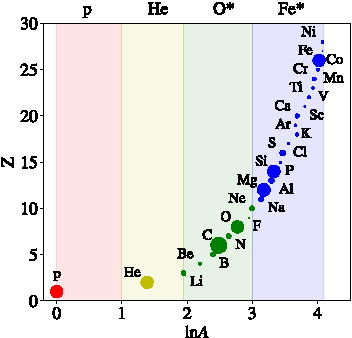
\includegraphics[width=0.5\textwidth]{./images/cosmic_ray_composition.pdf}
        \caption{Composition of the cosmic-rays grouped nearly equally in their logarithmic mass between proton and nickel. The size of the circles denotes the flux ratio compared to the leading element in each group. \cite{Dembinski17GSF}}
        \label{fig:cr_components}
        \vspace{0.5cm}
    \end{subfigure}
    \begin{subfigure}{0.9\textwidth}
        \centering
        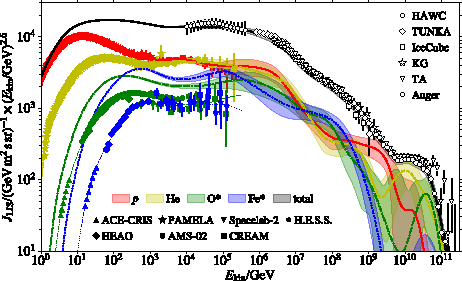
\includegraphics[width=\textwidth]{./images/cosmic_ray_spectrum.pdf}
        \caption{Global Spline Fit of the measured all-particle cosmic-ray energy spectrum. For Oxygen and Iron the data points represent the measured elemental flux and the model lines are shown without error bars for the elemental flux and with error bars for the group flux. \cite{Dembinski19MuonPuzzle}}
        \label{fig:cr_spectrum}
    \end{subfigure}
    \caption{The energy spectrum of the cosmic-rays from the GeV range to the GZK-cutoff. Up to a PeV, space-based detectors measure the cosmic-rays directly being able to differentiate between the compositions. Above a PeV, ground-based detectors measure the cosmic-rays indirectly via air showers.}
    \label{fig:cosmic_rays}
\end{figure}

\subsection{Cosmic-Ray Energy Spectrum}

The energy spectrum of incoming cosmic-rays, shown in \figref{fig:cr_spectrum}, is focusing above the GeV energy range where most of the particles are produced outside of our solar system.
Until energies of roughly a GeV the main source of measured cosmic-ray events originates from our sun with a variable event rate depending on the sun's activity.
Cosmic-rays from outside of our solar system are screened by the Heliosphere.

Above a GeV, the magnetic fields of the sun are not powerful enough to accelerate particles to such high energies and galactic sources are the main source of cosmic rays.
The main type of cosmic accelerators is considered supernova remnants (SNRs).
Supernov\ae{} occur on average once in a century in our galaxy, while their shock waves propagate hundreds of years into the interstellar medium.
The particles with these energies are considered to undergo the so-called Fermi acceleration, a shock acceleration resulting in a power-law spectrum $E^{-\gamma}$ with an index of $\gamma = \num{2}$.
Due to interaction losses and the probability to escape the galactic magnetic field the spectrum gets steeper and results in a measured spectral index of \num{2.7} on Earth.
SNRs can accelerate particles up to a PeV, a region called the \textit{knee} of the spectrum.

Above the \textit{knee} and until the so-called \textit{ankle} at an EeV yet unknown galactic sources, probably Pulsars or Quasars become dominant resulting in an increased measured spectral index of \num{3.1}.
Above the \textit{ankle} sources inside our galaxy are not powerful enough to accelerate such high energetic particles and extragalactic sources, e.g. Active Galactic Nuclei, become the main contributor.
The resulting spectral shape flattens again to an index of \num{2.6}.
At around \SI{1e20}{eV} the protons interact with the photons of the CMB to a Delta resonance, resulting in the GZK-cutoff of the energy spectrum, predicted by Greisen, Zatsepin and Kuz'man \cite{Greisen66GZK, Zatsepin66GZK}.

\subsection{Cosmic-Ray induced Air Shower} \label{sec:air_shower}

When cosmic-rays reach the Earth they interact with the dense medium of the atmosphere.
Depending on the energy and the composition of the particle, the height of the first interaction is at \SIrange{10}{15}{km}.
The secondary particles of this interaction again interact with the atmosphere resulting in a particle cascade or air shower that consists of thousands or even billions of particles.
These showers can be categorized into hadronic, muonic and electromagnetic shower components, which are illustrated in \figref{fig:air_shower_components}.

\begin{figure}
    \centering
    \begin{subfigure}[t]{0.58\textwidth}
        \centering
        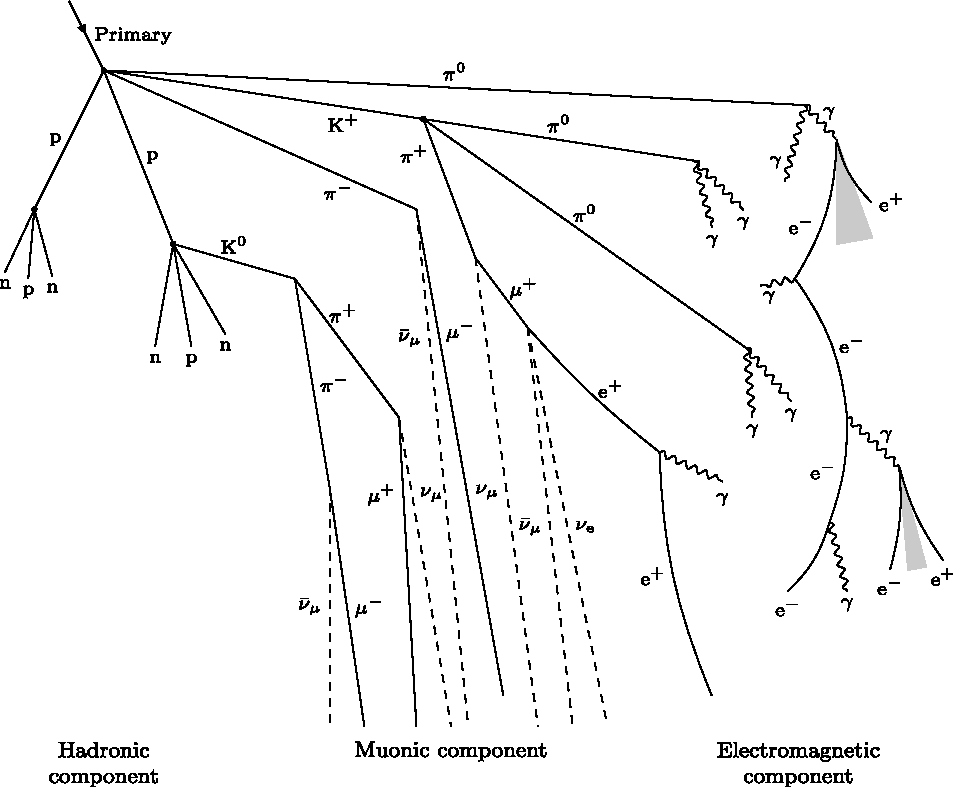
\includegraphics[width=\textwidth]{./images/air_shower_components.pdf}
        \caption{Basic scheme of the interactions and particles for the shower components of an air shower. Adapted from \cite{Krause15ICRC}}
        \label{fig:air_shower_components}
    \end{subfigure}
    \hfill
    \begin{subfigure}[t]{0.38\textwidth}
        \centering
        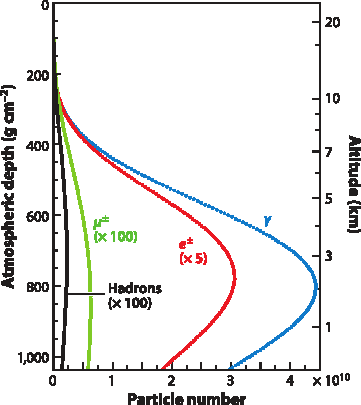
\includegraphics[width=\textwidth]{./images/air_shower_development.pdf}
        \caption{Development of the number of produced shower particles for a \SI{e19}{eV} proton induced vertical air shower. \cite{Engel11EAS}}
        \label{fig:air_shower_development}
    \end{subfigure}
    \caption{Development of a cosmic-ray induced air shower. To the left the different sub-showers divided into an electromagnetic, a muonic and a hadronic component is shown. To the right the contribution of these sub-showers and particles during the shower development is shown.}
    \label{fig:air_shower}
\end{figure}

\textbf{The electromagnetic shower component} consists of electrons, positrons and photons.
Starting e.g. with a high energy photon the two main gamma interactions are the production of an electron-positron pair, also called the Bethe-Heitler process, and Compton Scattering.
While the latter is just important for the deflection, the pair production is the important process for the shower development.
The produced electrons and positrons dominantly lose their energy via bremsstrahlung, creating again a high energy photon.
The Positron can also annihilate with the atomic electrons creating a photon pair, which is a sub-dominant process.

% (TODO: wie viel Energie geht in einem cyclus verloren? vgl Tau-Regeneration)
The cycle of photon pair production and electron/positron bremsstrahlung continues until the bremsstrahlung photons are below an MeV and therefore not energetic enough to create an electron/positron pair.
Due to the high number of charged particles (c.f. \figref{fig:air_shower_development}) that are created, this shower component produces the dominant amount of the Cherenkov light and is also important for the radio signal of a shower.
The production of a muon pair is a sub-dominant process as the muon mass is 200 times higher than the electron mass decreasing the phase space and is therefore not important for the electromagnetic shower development.
However, it is a non-negligible process regarding the number of produced muons inside the shower, while the main production originates from the hadronic shower.

\textbf{The hadronic shower component} mainly consists of the lightest mesons, charged Pions and Kaons ($m_{\pi^{\pm}} \approx \SI{140}{MeV}, m_{K^{\pm}} \approx \SI{494}{MeV}$ \cite{PDG20}).
Due to their relatively long lifetimes of $\tau_{\pi^{\pm}} = \SI{26}{ns}$ and $\tau_{K^{\pm}} = \SI{12}{ns}$, they propagate and lose a significant amount of their energy through interactions before they decay.
Pions decay mainly into muons, as their rest mass is just slightly higher.
Kaons either directly decay into muons (or electrons) or first decay into Pions, which then decay to muons and neutrinos.
The energy losses during the propagation of the Pions and Kaons lead to a steepening of the resulting muon and neutrino energy spectrum to a spectral index of \num{3.7}.
The muons or neutrinos originating from these processes are called \textit{conventional atmospheric} muons or neutrinos.

In addition to Pions and Kaons also short-lived mesons and baryons are produced in hadronic showers.
They consist mainly of mesons with a charm quark, like the D-Meson, of $\Lambda$-Baryons and unflavored mesons, while the latter do not often decay into muons and muon neutrinos.
Due to their short lifetime ($\tau \leq \SI{1}{ps}$), they do not lose energy during their short propagation and directly decay.
The resulting energy spectrum of the decay products is therefore similar to the primary spectrum as the spectral index does not change.
Although these processes are sub-dominant, the flatter spectral index of the resulting muons and neutrinos makes them relevant at higher energies.
Due to the direct decay of the hadrons, which mainly consist of charmed mesons, the resulting muons or neutrinos are called \textit{charmed} or \textit{prompt atmospheric} muons or neutrinos.

\textbf{The muonic shower component} mainly originates from the hadronic shower component and produces just a few secondaries compared to the other shower particles.
The high muon mass ratio compared to the electron also decreases the interaction probability as the bremsstrahlung cross section is proportional to $1/m^2$.
Combined with the relatively high lifetime, the muon range through dense media is the highest, neglecting neutrinos, making them the biggest background for all particle detectors even if they are located deep underground.
Except for detectors placed at high altitudes, they are the only shower component for inclined showers measured on the Earth's surface, neglecting the electromagnetic radiation like Cherenkov light, Fluorescence light or the radio signal.
The resulting muon and neutrino energy flux from cosmic-ray induced air showers is shown in \figref{fig:atmo_mu_nu_flux}.
\begin{figure}
    \centering
    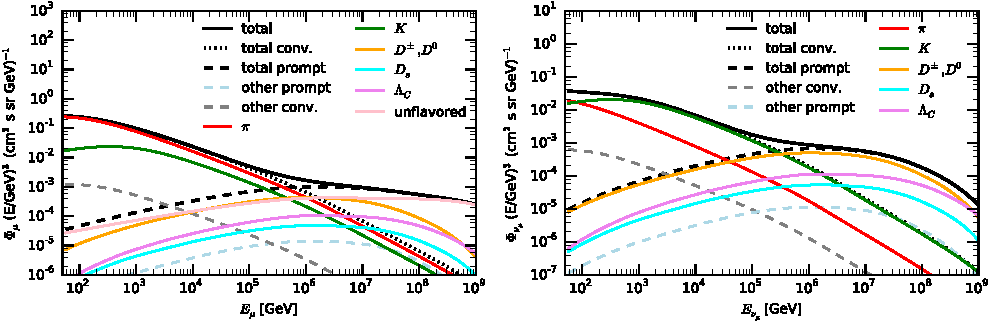
\includegraphics[width=\textwidth]{./images/mceq_mu_nu_flux.pdf}
    \caption{Predictions of the atmospheric muon and neutrino flux at the surface using matrix cascade equations. \cite{Fedynitch15MCEq}}
    \label{fig:atmo_mu_nu_flux}
\end{figure}

A longitudinal shower profile and the contribution of the different sub-shower types is shown in \figref{fig:air_shower_development}.
An increasing number of particles at the beginning of the shower development can be seen as well as a decreasing part when more and more bremsstrahlung photons are too low energetic to produce an electron-positron pair.
The resulting maximum of the longitudinal shower profile $X_{\mathrm{max}}$ at roughly \SI{5}{km} for vertical showers varies for the different primary particle types and energies making it an important feature to classify the primary particle.

Another important feature to estimate the energy of the primary particle is the number of muons detected at the Earth's surface.
Unfortunately, there is a discrepancy between the number of muons measured in air shower detectors, which exceeds the number of muons produced in air shower simulations starting at primary energies of \SI{e16}{eV} \cite{Dembinski19MuonPuzzle}.
That is seen across multiple experiments with a significance of \SI{8}{\sigma}, known as the \textit{Muon Puzzle} \cite{Albrecht21MuonPuzzle}.

It is considered, that most of the discrepancy arises from the uncertainties of the hadronic interaction models.
While most of the models are influenced by accelerator measurements from e.g. the LHC, these models provide good agreements for high transversal momentums.
In the forward direction, the beam pipe and not a detector is located, which is fine for those experiments as most differential cross sections diverge in the forward direction.
However, astroparticle physics experiments most often measure the shower in the forward direction leading to fewer cross-checks with the accelerator measurements.
This type of challenge to evaluate cross section also in the forward direction does not just occur for the hadronic models, but for all types of particle interaction including the muon cross sections.

A precise description of the muon bundles is also crucial for underground detectors to separate these background events from their signal.
While there are also muons with a high transversal momentum compared to the shower axis resulting in a lateral distribution \cite{Engel11EAS} most of the high energetic muons propagate close to the primary direction making a separation between them challenging.
An extraction of muon physics parameters out of these muon bundles is therefore limited and single muons are required to provide a deeper understanding.
% TODO: Plot showing the simulated muon arrival distribution of an air shower on the Earths surface. Ask DBaack

%
% 
% small seperation between the chapters
%
%

\section{Neutrino induced Muons}

Compared to the cosmic-ray induced muons that occur only in bundles, neutrinos produce single muons.
Further muons are produced in the hadronic cascade at the neutrino vertex or as muon pair production.
But these muons have much less energy and stop far before the main muon produced by the neutrino, so they can be neglected regarding muon energies of GeV or above.

\subsection{Neutrino Energy Spectrum}

The neutrino energy spectrum shown in \figref{fig:neutrino_spectrum} is assumed to starts with a high number of cosmological neutrinos or the cosmic neutrino background (C$\nu$B).
Like the CMB they are left-overs from the big bang when the temperature drops below the critical value of weak lepton production and annihilation.
It consists of all neutrino flavors but the energies are far too low to be measurable with current technology.
\begin{figure}
    \centering
    \includegraphics[width=0.8\textwidth]{./plots/nu_spectrum.pdf}
    \caption{The diffuse neutrino energy spectrum at the Earth from the cosmological neutrino background $C\nu B$ to cosmogenic neutrinos. The gap between the $C\nu B$ and the solar neutrinos from nuclear processes is filled by thermal solar neutrinos, not included here (c.f. \cite{Vitagliano20}). Adapted from \cite{KatzSpiering12}.}
    \label{fig:neutrino_spectrum}
\end{figure}

Until keV-energies, thermal neutrinos from the sun are predicted \cite{Vitagliano20} before at neutrino energies of keV and MeV solar neutrinos from fusion processes dominate the neutrino flux on Earth with additional contributions of terrestrial anti-neutrinos from naturally decaying radioactive nuclide.
Additional anti-neutrinos from nuclear reactors also contribute to the neutrino flux depending on the location on Earth \cite{Usman15}.
Although only electron neutrinos are produced in radioactive decays or fusion processes, solar neutrinos are measured in all three flavors through the neutrino oscillation further described in section \ref{sec:nu_osc}.

Furthermore in the MeV range neutrinos from supernova remnants also contribute to the neutrino flux.
For the last supernova, SN1987A, where the neutrino contribution was first measured, the neutrino flux was orders of magnitudes higher than the SNR flux, dominating the spectrum at MeVs during that burst.

For neutrino energies starting around a GeV cosmic-ray induced atmospheric neutrinos are the main contributors.
Their flux can be approximated by a broken power-law of \textit{conventional} and \textit{prompt} atmospheric neutrinos as described in section \ref{sec:air_shower}.
At around \SI{100}{TeV} both the prompt atmospheric and astrophysical neutrinos (probably from AGNs) starts dominating the flux both due to their flatter spectrum.
While the astrophysical flux has already been measured by IceCube, the prompt component has always been fitted to zero and its contribution remains hidden.

The neutrino creation process for the cosmic accelerators (possibly Active Galactic Nuclei) is similar to the atmospheric neutrinos.
Accelerated protons interact near the source and through the Pion and muon secondaries, neutrinos are produced.
In contrast to the atmospheric neutrinos, the medium at astrophysical sources is not as dense as the atmosphere and the Pions and muons do not lose much of their energy before they decay.
Therefore the energy spectrum does not get steeper and the spectral index remains on the level of the Fermi acceleration near 2.

The two main processes of the accelerated protons for the neutrino production are the $pp$-channel and the $p\gamma$-channel.
\begin{align}
    p p \to & \pi^+ \pi^- \dots \\
    p \gamma \to & \Delta^+ \to \begin{cases} \pi^+ n \\ \pi^0 p \end{cases}
\end{align}

In the $pp$-channel, a proton interacts with another proton in the surrounding matter near the source producing an equal amount of $\pi^+$ and $\pi^-$.
In the $p\gamma$-channel, a proton interacts with a photon producing a Delta-resonance resulting in the production of only positively charged Pions.
A way to distinguish between neutrinos and anti-neutrinos at these energies could therefore give further insights into the production processes \cite{Biehl17}.

Starting at \SI{10}{PeV} the so-called \textit{cosmogenic neutrinos} are predicted to be the main contributors.
They are produced from decaying Delta-resonances induced by cosmic-ray protons interacting with the CMB at the GZK-limit.
Unfortunately, they have not been measured yet, as the detectors to measure them with radio techniques are currently in the phase of planning and fund raising.

\subsection{Neutrino Flavors at Earth} \label{sec:nu_osc}

As already mentioned for solar neutrinos, the primary electron neutrino flux on Earth is measured in all three neutrino flavors due to neutrino oscillation \cite{SNO01Oscillation}.
The distance between the Earth and the sun is greater than the oscillation length for neutrinos at these energies.
For an initial electron neutrino flux, the oscillations lengths for the lepton flavors are shown in \figref{fig:nu_osc_len}.
Also for terrestrial distances neutrino oscillation is measurable e.g. for atmospheric neutrinos, where the flavor composition depends on the zenith angle \cite{SK98Oscillation}.
The neutrino propagating through the Earth further changes due to the different oscillation behavior between the propagation through matter compared to vacuum (MSW effect) \cite{Mikheyev85, Wolfenstein79}.
\begin{figure}
    \centering
    \begin{subfigure}[t]{0.47\textwidth}
        \centering
        \includegraphics[width=\textwidth]{./plots/nu_osc_len.pdf}
        \caption{Oscillation length for an initial electron neutrino flux into the three neutrino flavor.}
        \label{fig:nu_osc_len}
    \end{subfigure}
    \hfill
    \begin{subfigure}[t]{0.47\textwidth}
        \centering
        \includegraphics[width=\textwidth]{./plots/nu_flavor_triangle.pdf}
        \caption{Neutrino flavor triangle for different source scenarios.}
        \label{fig:nu_flavor_trangle}
    \end{subfigure}
    \caption{Neutrino flavor ratios for different observation distances to the source. To the left one full oscillation length is shown and on the right the average of the oscillation periods is shown. The currently measured oscillation parameters \cite{PDG20} and  an inverted mass hierarchy as this is slightly favored is used.}
    \label{fig:nu_osc}
\end{figure}

For astrophysical sources like SNRs or AGNs, the propagation distances are much larger than the oscillation length and the mean probability averaged over the oscillation is used to describe the neutrino flux composition depending on the initial production composition.
There are three mainly discussed production scenarios describing one likely and two extreme scenarios of neutrino production.

Assuming pure \textbf{pion decay} processes, the flavor ratio $\nu_e : \nu_{\mu} : \nu_{\tau}$ is $1:2:0$
\begin{align}
    \pi^+ \to &\mu^+ \nu_\mu \\
    &\mu^+ \to e^+ \nu_e \bar{\nu}_{\mu} ,
\end{align}
Equivalent processes happen for the $\pi^-$ decay.

In the \textbf{muon damping} model, also assuming pure pion decays, the produced muons interact near the production region and lose most of their energy before they decay assuming a more dense medium around the source.
The outgoing neutrinos of the muon decay are therefore in the range of a few MeV which is not measurable for astroparticle detectors.
The resulting flavor ratio of $0:1:0$ then does not contain electron neutrinos.
Atmospheric electron neutrinos are mainly produced in Kaon decay as Kaons decay equally into muons and electrons.

In the other extreme scenario, a high energy \textbf{neutron beam} is assumed at the source.
In the decay of the neutrons, a pure electron neutrino flux with a flavor ratio of $1:0:0$ is produced.

For all three neutrino production scenarios, the flavor ratio that would be measured on earth after averaging over the neutrino oscillation is shown in \figref{fig:nu_flavor_trangle}.
Independent of the neutrino creation model at the astrophysical source, neutrinos of all three flavors will arrive at the earth through neutrino oscillation, including tau neutrinos.
The most discussed scenario of the dominating pion production without muon damping produces a nearly equal amount of $1:1:1$.

Tau neutrinos are of special interest since the rate for direct production of the tau lepton with its high mass of \SI{1.7}{GeV} is highly suppressed; both in air showers and at extragalactic sources.
They are only measurable through neutrino oscillation and have therefore high confidence being of astrophysical origin.

Due to the negligible initial tau neutrino flux, the currently measured oscillation parameters assuming the standard model allows the neutrino flavor arriving on earth just to be in a distinct region of the flavor ratio, shown in \figref{fig:nu_flavor_trangle}.
A precise measurement of the neutrino flavors could limit the allowed source scenarios.

The tau lepton, produced during the neutrino interaction as described in the following section, also decays into muons making them a non-negligible source of neutrino-induced muons.

\subsection{Neutrino Interactions}

There are three different interaction modes, illustrated in \figref{fig:feyn_nu}, on how neutrinos can interact with matter.
\begin{figure}
    \begin{subfigure}{0.31\textwidth}
        \centering
        %
\begin{tikzpicture}
\begin{feynman}
    % define vertices
    % muon
    \vertex (nu_in) at (-\feynlen, \feynlen);
    \vertex (nu_vertex) at (0, 0.75*\feynlen);
    \vertex[right=2*\feynlen of nu_in] (l_out);
    % nucleus
    \vertex[below=1.5*\feynlen of nu_in] (n_in);
    \vertex[below=\feynlen of nu_vertex] (n_vertex);
    \vertex[below=1.5*\feynlen of l_out] (n_out);
    % draw diagram
    \diagram* {
        (nu_in) -- [fermion] (nu_vertex) -- [fermion] (l_out),
        (nu_vertex) -- [boson, edge label=$W^\mp$] (n_vertex)
    };
    % draw extra features with tikz (not available in tikz-feynman)
    \draw[thick, double] (n_in) -- (n_vertex) -- (n_out);
    \draw[fill] (nu_vertex) circle[radius=\feynvertexsize];
    \draw[fill] (n_vertex) circle[radius=\feynvertexsize];
    % add labels
    \node[left] at (nu_in) {$\nu_{l^\pm}$};
    \node[right] at (l_out) {$l^\pm$};
    \node[left] at (n_in) {$N$};
    \node[right] at (n_out) {$X$};
\end{feynman}
\end{tikzpicture}
%
        \caption{Charged Current (CC)}
        \label{fig:feyn_nu_cc}
    \end{subfigure}
    \hfill
    \begin{subfigure}{0.31\textwidth}
        \centering
        %
\begin{tikzpicture}
\begin{feynman}
    % define vertices
    % muon
    \vertex (nu_in) at (-\feynlen, \feynlen);
    \vertex (nu_vertex) at (0, \feynlen-\feynsmallen);
    \vertex (nu_out) at (\feynlen, \feynlen);
    % nucleus
    \vertex (n_in) at (-\feynlen, -\feynlen);
    \vertex (n_vertex) at (0, -\feynlen+\feynsmallen);
    \vertex (n_out) at (\feynlen, -\feynlen);
    % draw diagram
    \diagram* {
        (nu_in) -- [fermion] (nu_vertex) -- [fermion] (nu_out),
        (nu_vertex) -- [boson] (n_vertex)
    };
    % draw extra features with tikz (not available in tikz-feynman)
    \draw[thick, double] (n_in) -- (n_vertex) -- (n_out);
    \draw[fill] (nu_vertex) circle[radius=\feynvertexsize];
    \draw[fill] (n_vertex) circle[radius=\feynvertexsize];
    % add labels
    \node[left] at (nu_in) {$\nu$};
    \node[right] at (l_out) {$\nu'$};
    \node[right] at (0,0) {$Z^0$};
    \node[left] at (n_in) {$N$};
    \node[right] at (n_out) {$X$};
\end{feynman}
\end{tikzpicture}
%
        \caption{Neutral Current (NC)}
        \label{fig:feyn_nu_nc}
    \end{subfigure}
    \hfill
    \begin{subfigure}{0.31\textwidth}
        \centering
        %
\begin{tikzpicture}
\begin{feynman}
    % define vertices
    \vertex (nu_in) at (-\feynlen, 0.75*\feynlen);
    \vertex (e_in) at (-\feynlen, -0.75*\feynlen);
    \vertex (nu_vertex) at (0, 0);
    \vertex[right=\feynlen of nu_vertex] (w_out);
    % draw diagram
    \diagram* {
        (e_in) -- [fermion] (nu_vertex) -- [fermion] (nu_in),
        (nu_vertex) -- [boson] (w_out)
    };
    % draw extra features with tikz (not available in tikz-feynman)
    \draw[fill] (nu_vertex) circle[radius=\feynvertexsize];
    % add labels
    \node[left] at (nu_in) {$\bar{\nu}_e$};
    \node[left] at (e_in) {$e^-$};
    \node[right] at (w_out) {$W^-$};
\end{feynman}
\end{tikzpicture}
%
        \caption{Glashow Resonance}
        \label{fig:feyn_glashow}
    \end{subfigure}
    \caption{The feynman diagrams of the most dominant neutrino interactions at high energies.}
    \label{fig:feyn_nu}
\end{figure}

The \textbf{Charged Current} (CC) interaction, with a W-boson as the exchange particle between the nucleon and the neutrino, is the main producer of high energy muons.
While the neutrino converts into its charged counterpart-lepton the other outgoing product is the hadronic cascade.
The \textbf{Neutral Current} (NC) Interaction, with a Z-boson as the exchange particle, just produces an energy loss of the neutrino without converting it.
Therefore only the hadronic cascade is the visible outcome of this interaction.
For both the CC and NC interactions on average a third of the neutrino energy is stored as hadronic cascade and two-thirds in the outgoing lepton, shown in \figref{fig:nu_xsection_y}.

The CC interaction is the dominant interaction contributing two-thirds to the total cross section, while the NC just contribute a third, as shown in \figref{fig:nu_xsection_tot}.
For lower energies, the anti-neutrino cross section is smaller as the valence quarks are the main interaction partners.
The sea quarks and thereby an equal treatment of neutrino and anti-neutrino become more important at higher energies.

\begin{figure}
    \centering
    \begin{subfigure}[t]{0.47\textwidth}
        \centering
        \includegraphics[width=\textwidth]{./plots/nu_xsection_tot.pdf}
        \caption{Total neutrino cross section}
        \label{fig:nu_xsection_tot}
    \end{subfigure}
    \hfill
    \begin{subfigure}[t]{0.47\textwidth}
        \centering
        \includegraphics[width=\textwidth]{./plots/nu_xsection_average_y.pdf}
        \caption{Average energy loss to the hadronic cascade relative to the neutrino energy.}
        \label{fig:nu_xsection_y}
    \end{subfigure}
    \caption{Neutrino cross section for the Charged Current (CC) the Neutral Current(NC) and the Glashow Resonance(GR). For the CC and NC interaction, the calculation from \cite{CSMS11NuXsection} and for the Glashow resonance, the parametrization of \cite{Barger14} are used.}
    \label{fig:nu_xsection}
\end{figure}

At an energy of \SI{6.3}{PeV}, the peak of the \textbf{Glashow Resonance} (GR) dominates the cross section \cite{Glashow60}.
At this energy, the anti-electron neutrino interacts resonantly with an atomic electron producing a $W^-$-boson.
The result is a huge hadronic cascade, as the W-Boson decays with the hole energy, producing also multiple higher energetic muon tracks characteristic for this interaction.
Next to the hadronic decay mode in $\sfrac23$ of the cases, the remaining third is equally distributed on the three leptonic decay modes.
Although the resulting muons are challenging to identify, a first candidate of a high energetic muon originating from a Glashow resonance has been found \cite{IceCube2016Aachen}.

The energy distribution of muons propagating out of a hadronic cascade is described in \cite{Panknin09ICRC}.% shown in \figref{fig:mu_flux_hadr_shower}.
Compared to the directly produced muon of the CC interaction, the secondary muons of the hadronic cascade are much less energy while still producing a non-negligible signature.
Especially, as the hadronic interactions not only occur at the neutrino vertex but also at each inelastic nuclear interaction along a muon track.
% \begin{figure}
%     \centering
%     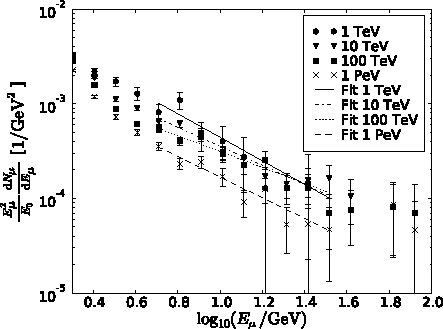
\includegraphics[width=0.8\textwidth]{./images/muon_flux_hadronic_shower.pdf}
%     \caption{Differential muon flux for several injected hadronic energies. \cite{Panknin09ICRC}}
%     \label{fig:mu_flux_hadr_shower}
% \end{figure}

% \chapter{Muon Detection} \label{sec:detection}

Muons can be measured by the energy losses along their propagated track, each producing a particle cascade.
While the bare muon also produces a signal, the main signature is produced by the secondaries of the energy losses.
Here the main detection techniques of muons for cosmic-ray detectors and neutrino telescopes are presented.

\section{Detection principles}

The \textbf{Cherenkov Effect} \cite{Cherenkov34} describes the optical light produced by a charged particles propagating faster than the speed of light through a medium.
Due to the through-going charged particle, the medium gets polarized and creates a signal.
These signals are emitted coherently when the charged particle propagates faster than the speed of light in this medium, creating a Cherenkov cone with an opening angle of $\cos \theta = 1/\beta n$ similar to a hypersonic cone of an Airforce jet.
$n$ is the refraction index that also depends on the wavelength.
The Frank-Tamm formula \cite{FrankTamm37} describing the spectrum of the emitted Cherenkov photons has a $1/\lambda^2$ dependency, with the wavelength $\lambda$, and is therefore UV-divergent (neglecting the suppressing contribution of the refraction index).
Focusing on the optical wavelength and the medium ice, around \num{400} Cherenkov photons are emitted per centimeter with the main contribution of around \SI{400}{nm} (blue light).
The energy loss caused by the Cherenkov effect is around \SI{170}{eV/cm} which is four orders of magnitudes below the minimum Ionization loss of \SI{2}{MeV.\per.cm} and is therefore negligible for the energy loss during the propagation.
The Cherenkov light can be measured with Photomultiplier Tubes (PMTs) with the advantage of a wide collection area useful in water tanks but with the disadvantage of demanding high voltages.
Alternatively, the light can be measured with Silicon Photo Multiplier (SiPM) being able to operate without high voltages but only having a small collection area and therefore only applicable when the light is guided to them.

The \textbf{Askaryan Effect} \cite{Askaryan62} describes the radio signal caused by the relativistic propagation of a particle cascade.
In principle, the radio signal is produced by the geomagnetic and the Askaryan effect, but it is commonly known as the Askaryan effect.
The geomagnetic effect describes the separation of positrons and electrons during an electromagnetic cascade due to the geomagnetic field.
Due to the high number of shower particles, this creates a dipole perpendicular to the shower axis changing over time as the shower increases to its $X_{\text{max}}$ and then decreases.
Since there are only atomic electrons and no positrons, these electrons of a medium get knocked-out by the shower particles and the shower front gets charged negatively leaving the positively charged ions behind.
This charge imbalance along the shower axis is also changing over time as the shower develops which is considered as the Askaryan effect.
Both effects are just measurable because the particle cascade propagates faster than the speed of light in the medium thus producing a coherent radio signal at the Cherenkov angle.
For air showers, the radio signal is mainly produced by the geomagnetic effect while for more dense media, like ice, the Askaryan effect produces the dominant radio signal.
Only the highest energetic particle showers ($>\si{EeV}$) produce a sufficient amount of electrons and positrons and thereby a detectable radio signal.
The energy loss of \SI{18}{MeV} for an EeV shower due to this effect is even more negligible compared to the Cherenkov radiation.
The radio signal with wavelengths of a meter has a much higher attenuation length of about a kilometer in ice compared to \SI{100}{m} for optical light.

Even before the radio signal, Askaryan predicted an \textbf{acoustic signal} produced by high energetic cascades \cite{Askaryan57Acoustic}.
The huge amount of high energy charged particles inside the small shower region increases the energy and thereby the temperature of the medium in this area.
The heated region expands and creates an acoustic wave with a maximum frequency at \SI{10}{kHz}.
Through the coherent superposition of the sound waves, an acoustic signal perpendicular to the particle shower is produced that can be measured \cite{Lahmann16Acustic}.
Similar to the radio signal the attenuation length is on the order of a kilometer making both techniques interesting for rare events requiring huge detection volumes.

The \textbf{fluorescence effect} in general describes atoms or molecules that get excited and thus emitting optical light.
In the context of particle detectors, this is mainly used in scintillator detectors where the charged particle excites the scintillator material when passing through which emits light.
While the scintillation area can have a size of $\mathcal{O}(m^2)$, the emitted light can then be guided to a detector that just needs a small collection area, like an SiPM.
Besides this use of the fluorescence effect, the fluorescence light is used in the detection of the excited nitrogen molecules in the atmosphere caused by the huge number of high energetic particles in the shower \cite{Keilhauer12Fluorescence}.
The emitted fluorescence light at each shower depth is equivalent to the energy loss per distance making the energy of the shower extractable via the integral of the longitudinal shower profile.
Another type is the luminescence light which is used in searches of magnetic monopoles with neutrino telescopes, where the radio-luminescence induced by these highly ionizing particles has become a field of research \cite{Pollmann19Luminescence}.

%
% 
% small seperation between the chapters
%
%

\section{Air Shower Detectors}

The different signals an air shower produces are measured with multiple approaches, from the direct detection of the different shower particles at high altitudes over the muon detection at the surface to the fluorescence or radio signal besides the shower axis.

\subsection{Gamma-Ray induced Air Shower Detectors}

Extended air shower Arrays (EAS-Arrays) are placed at high altitudes, ideally near the typical maximum of the shower profile $X_{\mathrm{max}}$ to measure most of the produced particles inside the detector.
One approach is using a dense array of closed tanks filled with purified water.
Through-going charged particles of the shower produce Cherenkov light inside the water, which can be detected with optical sensors mainly PMTs.
Currently, the most sensitive observatory is the HAWC detector \cite{HAWC17} operating at an altitude of \SI{4.1}{km} above sea level (asl) in the Sierra Negra, Mexico.
Inside an area of \SI{22000}{\square\meter}, 300 cylindric tanks are placed each containing around \SI{200}{\cubic\meter} of water with 4 PMTs at the bottom measuring the Cherenkov light.
The upcoming LHAASO experiment in Tibet \cite{LHAASO19} will increase the sensitivity for air showers due to the higher altitude at \SI{4400}{m} asl.
Although EAS-Arrays are mainly designed to measure $\gamma$-ray induced air showers, one can also use them to analyze cosmic-ray induced showers in the PeV range around the \textit{knee} \cite{HAWC17CRSpectrum}.
Muons can be identified as they reach the ground of the detector producing light along their full track, while electrons will lose nearly all of their energy during their propagation through around \SI{4}{m} of water from the top of a tank to the bottom creating a uniform light pool.

Another type of telescope that was mainly developed for gamma astronomy but is also used to study cosmic-ray physics are imaging air Cherenkov telescopes (IACTs).
The detection techniques of both types of gamma telescope designs are illustrated in \figref{fig:detect_swgo}.
Hereby, the relativistic particles of an air shower are not measured directly, but indirectly via the Cherenkov light, they produce in the atmosphere, which can be also measured at moderate altitudes.
The current most sensitive telescopes are the HESS \cite{HESS20}, MAGIC \cite{MAGIC16II} and VERITAS \cite{VERITAS15Science} telescopes operating at \SI{1800}{m} \SI{2200}{m}, \SI{1300}{m} asl. respectively.
Electromagnetic or hadronic showers produce elliptical camera pictures with an additional spread-out for hadronic showers due to the higher transverse momentum of the hadronic interaction products.
Compared to that, muons produce a ring-like signature when propagating to the ground near the telescope.
Using this unique signature, IACT arrays measuring the same hadronic shower in multiple telescopes as well as the muons can give further insights into the muon flux produced in air showers \cite{Mitchell19MuonIACT}.
However, this approach will only work with an array of many telescopes as will be built in the upcoming CTA observatory \cite{CTA19Science}.
Compared to the closed tanks of EAS-Arrays with a duty cycle of nearly \SI{100}{\%}, IACTs can only operate at clear, moonless nights limiting their duty cycle to \SI{20}{\%}.
\begin{figure}
    \centering
    \begin{subfigure}{0.9\textwidth}
        \centering
        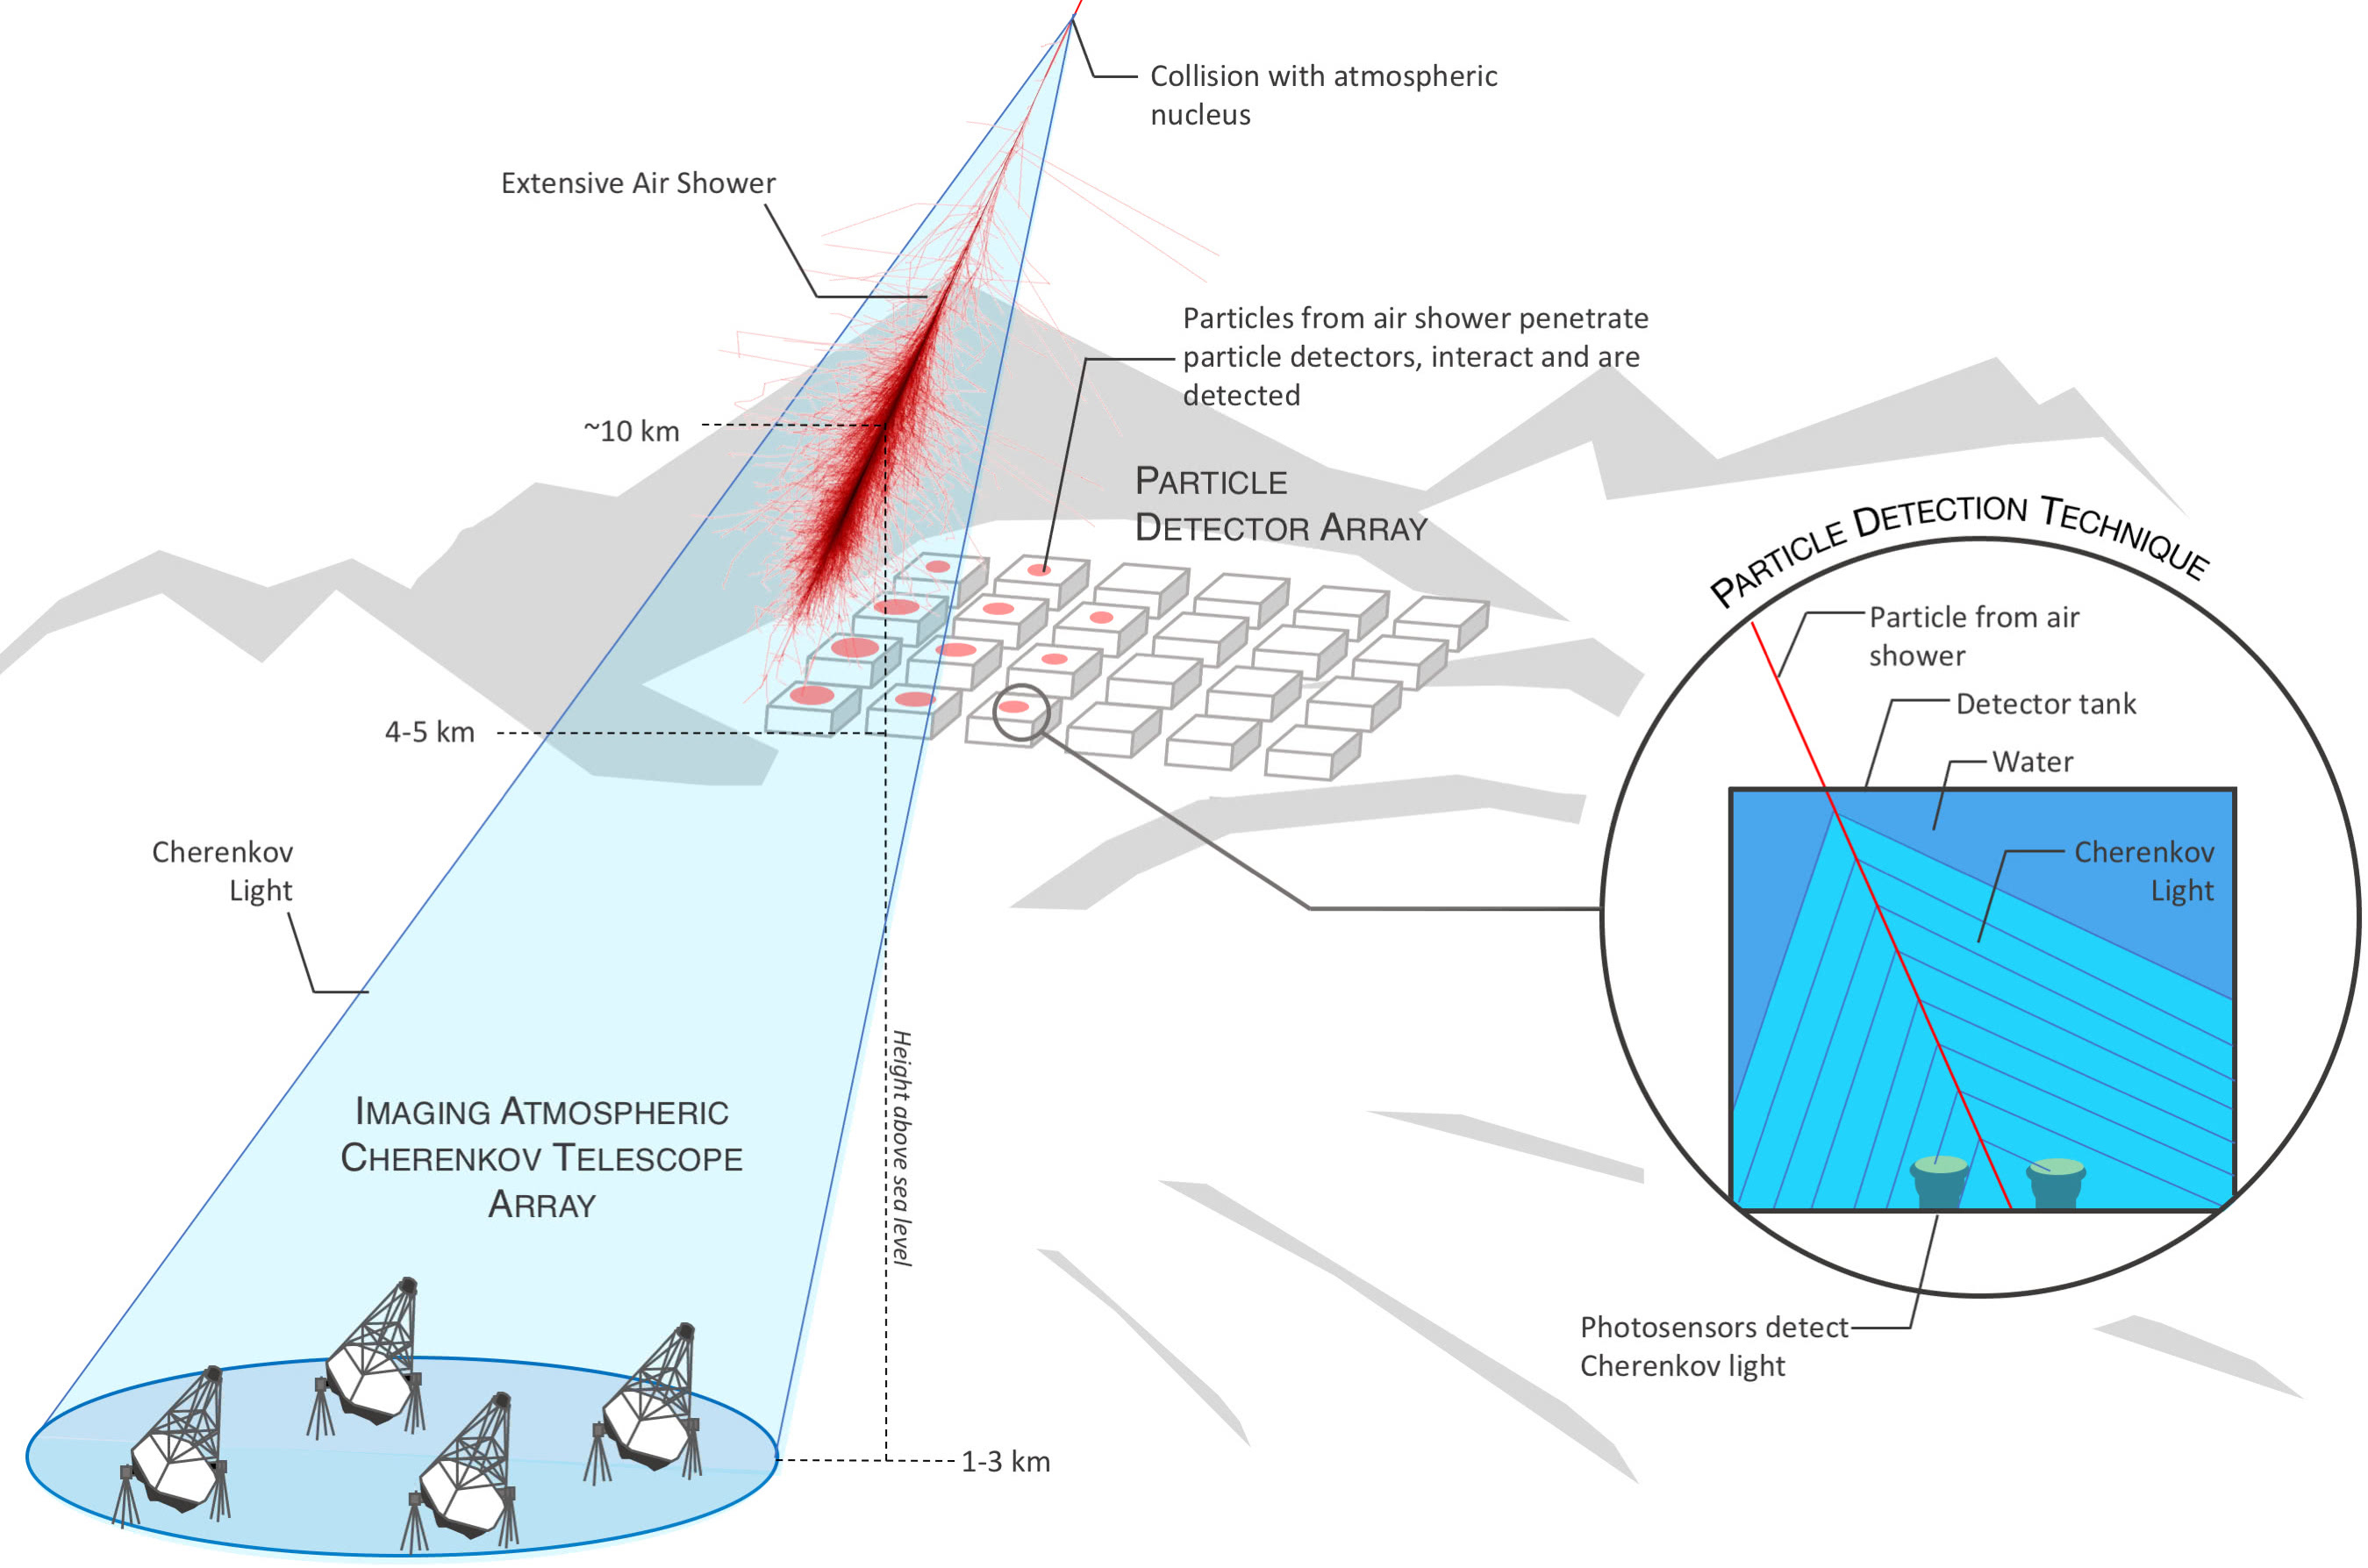
\includegraphics[width=\textwidth]{./images/detector_swgo.jpg}
        \caption{Direct particle detection at high altitudes with an extended air shower array and Imaging Air Cherenkov Telescopes at lower altitudes detecting the produced Cherenkov light in the atmosphere. \cite{SWGO19}}
        \label{fig:detect_swgo}
    \end{subfigure}
    \begin{subfigure}{0.7\textwidth}
        \vspace{0.5cm}
        \centering
        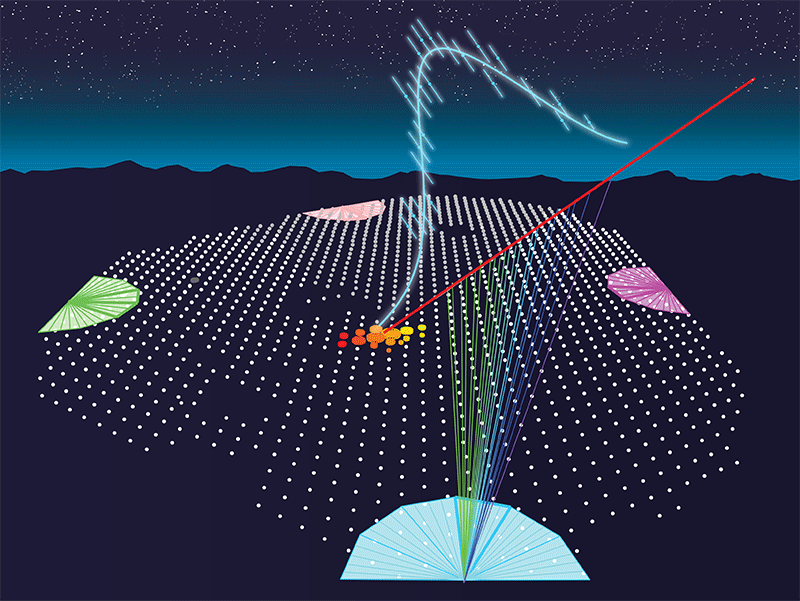
\includegraphics[width=\textwidth]{./images/detector_auger.png}
        \caption{Air shower measurement techniques of the Pierre-Auger Observatory using surface detectors and Fluorescence detectors. \cite{Gaisser16Auger}}
        \label{fig:detect_auger}
    \end{subfigure}
    \caption{Air shower measurement techniques using direct particle detection at high altitudes with an extended air shower array and the produced Cherenkov light in the atmosphere using Imaging Air Cherenkov Telescopes.}
    \label{fig:detect_air_shower}
\end{figure}

\subsection{Cosmic-Ray induced Air Shower Detectors}

Also at these moderate altitudes, it is possible to measure the fluorescence light produced mainly by the electromagnetic component of an air shower.
As these fluorescence detectors can cover a large effective area, rare events like the cosmic-rays at the GZK cut-off can be measured.
Currently, the most sensitive experiments for this type of detection are the Telescope Array \cite{TA12FD, TA13SD} in Utah observing the northern hemisphere and the Pierre Auger Observatory \cite{Auger15} in Argentina for the southern hemisphere both operating at around \SI{1400}{m} asl.
The Pierre Auger Observatory, shown in \figref{fig:detect_auger} consists of 24 fluorescence telescopes and 1500 Water Cherenkov Tanks on an area of \SI{300}{\square\kilo\meter} each containing \SI{12}{\cubic\meter} water and 3 PMTs.

Combining the fluorescence detection with an array of surface detectors sparsely placed on a large area to measure the particles reaching the ground has become a successful approach to measure the highest cosmic-rays.
In this hybrid method, the fluorescence detectors measure the longitudinal profile of the shower and thereby the energy of the shower.
The surface detectors measure the electromagnetic component only for vertical showers or just the muonic component for inclined showers being sensitive to the mass composition of the cosmic-ray.
While the surface detectors have a full duty cycle, the fluorescence detectors can only operate at clear nights, similar to the IACTS and EAS-Arrays and their duty cycles.
In combination with the lateral shower profile and its arrival times measured by the surface detectors, the main information of the primary particle, composition, energy and direction can be reconstructed.
Unfortunately, discrepancies in the number of muons between the measurement and the prediction of the simulation limit the use of Monte-Carlo based analysis and therefore the sensitivity on the mass composition.

Recent developments for the Pierre Auger Observatory \cite{Auger16Prime, Castellina19Prime} also include the usage of scintillator detectors at the surface, which are more sensitive to the electromagnetic component while being less sensitive to the nearly horizontal propagating muons of inclined showers.
Also part of this upgrade is placing radio antennas at each station to detect the radio signal thus measuring more components of the shower to better reconstruct the particle shower.

\subsection{Further Detectors measuring Atmospheric Muons}

A transit between a cosmic-ray induced muon detector and a neutrino detector is the NEjtrinnyj VOdnyj (Water) Detektor, NEVOD \cite{NEVOD15} located inside a building  at the MePhI in Moscow.
The detector, shown in \figref{fig:detect_nevod}, consists of a water-filled chamber with a size of $\SI{9}{m} \times \SI{9}{m} \times \SI{26}{m}$.
Inside this indoor pool, 25 Strings each containing three or four Quasi-Spherical-Modules which themselves consist of six PMTs looking in all three orthogonal directions, forward and backward and measure the light of the muons propagating through the chamber.
Due to the three-dimensional detector structure, the muons are not just registered, but also their energy loss behavior can be measured.
To increase the angular resolution for horizontal events, the DECOR enhancement was built consisting of streamer tube chambers at the sidewalls of the detector.
The high sensitivity on horizontal air showers and muon bundles makes this detector unique to analyze atmospheric muons and the Muon-Puzzle.
Next to the measurement of atmospheric air showers, NEVOD can detect neutrinos selecting upward-going events.
\begin{figure}
    \centering
    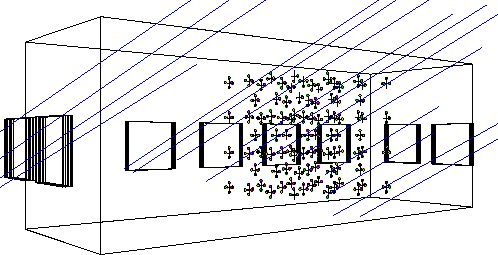
\includegraphics[width=\textwidth]{./images/detector_nevod.pdf}
    \caption{Sketch of the NEVOD-DECOR detector consisting Quasi-Spherical-Modules. \cite{NEVOD18}}
    \label{fig:detect_nevod}
\end{figure}

Another field of research detecting atmospheric muons with applications outside of the particle physics is the muon tomography.
Using the attenuation of the muon flux that varies between different materials, larger volumes of unknown material can be detected.
Application areas are the detection of varying magma chambers leading to a prediction of an eruption sequence of a volcano \cite{Tanaka09} or the detection of an unknown chamber in the Cheops pyramid \cite{Morishima17}.
Further applications are the measurement of large-angle Coulomb scattering to detect materials with high atomic numbers \cite{Borozdin03}.
Those detectors consist of several layers of plastic scintillators with the size of some \si{m^2} each passing the light to an SiPMs to track the number of muons and their direction.
An overview of the current muon imaging tools is reviewed in \cite{Bonechi19}.

So far, only experiments at the surface have been discussed measuring the muonic shower component as part of the signal or the main signal.
For most experiments located deep underground atmospheric muons are considered as background and not used to study cosmic ray physics, but to search for rare events like proton decays or Dark Matter interactions.
An exemplary detector for Dark Matter is the PICO detector \cite{Amole19PICO} in the Sudbury mine in Canada \SI{2}{km} below the surface, which equals \SI{6}{kmwe}.
Inside a pressure vessel with a diameter of \SI{60}{cm} and a height of \SI{167}{cm} superheated liquid C$_3$F$_8$ is used to measure small recoil energies (\SIrange{1}{100}{keV}) induced by elastic scattering of Weakly Interacting Massive Particles (WIMPs), a candidate for Dark Matter.
The main background limiting the sensitivity is not the atmospheric muons themselves, but the neutrons produced in interactions near the detector after propagating all the way down.
For these types of experiments, a precise description of the angular and energy distribution of the muon flux is crucial, especially the probability to reach those depths for inclined muons traveling even greater distances through the rock.
Therefore, the physical models need to be calculated and simulated with high precision, even for the edge cases of the stochastic propagation.
An exemplary detector for proton decay was the Fr\'{e}jus-Detector \cite{Frejus95nu} located \SI{4800}{mwe} under the Col du Fr\'{e}jus.
The calorimetric detector of the size () used iron to track particle interactions inside the detector.
Although a proton decay had not been measured, atmospheric muons had been used to create a depth curve and also the energy spectrum of atmospheric neutrinos had been unfolded.

%
%
% small seperation between the chapters
%
%

\section{Neutrino Detectors}

Besides the NEVOD Detector, most neutrino detectors are located deep underground to exclude the dominating background of atmospheric muons.
The low interaction rate of neutrinos is on the one side an advantage as it increases the observable horizon and let them propagate even through dense media like the core of the earth.
On the other side, this makes them challenging to detect and a large volume of detector material is required.
Due to the steep power-law dependence of the energy flux the energy range of the neutrinos scales with the size of the detection volume.
Four main types of neutrino telescopes have been established so far.

%  use the Cherenkov light emitted by charged secondary particles to measure neutrinos.
% Large volumes of media transparent to the blue Cherenkov light like Water, Ice or simply the air is used as a detection volume.
% Other methods like the radio or acoustic detection are in the development phase.

\subsection{Types of Neutrino Telescopes}

An exemplary detector in the neutrino energy range from MeV to \SI{10}{GeV} is the Super-Kamioka Neutrino Detection Experiment \cite{HyperKamiokande18} located in a former mine \SI{1}{km} deep underground in Japan.
It consists of a cylindrical tank with \SI{40}{m} in diameter and height filled with \SI{50}{kt} of purified water.
The Cherenkov light produced by particles interacting inside this tank is measured with \num{13000} PMTs positioned at the walls.
This peripheral detector type is used, since the absorption length of the Cherenkov radiation is larger than the detector size.
Similar structures for this energy range are SNO \cite{SNO20}, BOREXINO \cite{Borexino09} and JUNO \cite{JUNO19}, all located deep underground with several kt of liquid and transparent detector material, water or liquid scintillator and the PMTs at the walls.

To detect neutrinos with energies above \SI{10}{GeV} larger detector volumes with an effective radius of $\mathcal{O}(\SI{100}{m})$ are required.
These volumes can just be reached by using natural resources and placing the detectors inside the water, i.e. glacial ice, deep lakes or the sea.
Those distances exceed the absorption lengths of the Cherenkov light for water and a lattice structure of the detector is used.
Currently, the largest and most sensitive detector is the IceCube Neutrino Observatory at the South Pole with a detection volume of a cubic kilometer, which is further described in section \ref{sec:IceCube}.
Inside a detection volume of a cubic kilometer, the Cherenkov light produced by neutrinos or atmospheric muons is measured with around 5000 PMTs.
Therefore this type of telescope is labeled \textit{Cherenkov Neutrino Telescope}.
Further neutrino telescopes using the detection principle like IceCube are the ANTARES/Km3Net \cite{ANTARES11, KM3Net16} experiment in the Mediterranean sea, the Baikal/GVD in Lake Baikal \cite{Baikal97, GVD19} and the P-ONE experiment in the Cascadia Bassin in front of Vancouver \cite{PONE20}.
Compared to IceCube these telescopes are all upgrading to a volume of a cubic kilometer, are all located in the northern hemisphere and all use liquid water as detection volume.
Although the detection media is always water-based, the propagation of the Cherenkov light mainly described by the scattering and absorption differs significantly, as shown in \tabref{tab:len_abs_scat}.
While a strong absorption leads to the loss of photons and worse energy measurements, a strong scattering delays the photons and leads to a loss of directional information.
\begin{table}
    \caption{Characteristic lengths of absorption $\lambda_{\text{abs}}$ and scattering $\lambda_{\text{scat}}$ for selected locations with a Cherenkov-based neutrino detector. For detectors in liquid water, the range indicates the seasonal variation. The scattering lengths are corrected for the average Mie-Angle of the medium $\lambda_{\text{eff}}=\lambda_{\text{scat}}/(1-\langle\cos \theta\rangle)$. (TODO: cite private communication from Olga at Astropatricle School 2016 in Bad Honnef, find better source)}
    \label{tab:len_abs_scat}
    \begin{center}
    \begin{tabular}{l c c c}
        \toprule
        Location & Depth / km & $\lambda_a$ / m & $\lambda_{\text{eff}}$ / m \\
        \midrule
        Lake Baikal & $\sim 1$ & 22 & 150-400 \\
        Mediterranean Sea & $> 1.5$ & 40-70 & 200-400 \\
        South Pole & $1.5 - 2$ & 110 & 25 \\
        South Pole & $2 - 2.5$ & 220 & 47 \\
        \bottomrule
    \end{tabular}
    \end{center}
\end{table}

With this type of neutrino telescopes neutrinos with energies up to \SI{10}{PeV} can be measured.
Also with the planned IceCube-Gen2 detector increasing the size by a factor of ten \cite{IceCube20Gen2} the expected flux of the highest energetic neutrinos is too low to be detectable.
However, similar to the Pierre-Auger Observatory a maximum size of this type of detector is reached with Gen2.
To detect even higher energetic neutrinos and analyze the predicted cosmogenic neutrinos, detectors measuring the radio signal are under development.
Because of the long wavelength, these radio pulses can propagate several kilometers through the ice.
Therefore these detectors can be placed sparsely and cover a cubic kilometer with just a single station.
There are currently two attempts to build a Radio-Neutrino Detector; one as part of IeCube-Gen2 in the Antarctic Ice and another one on Greenland \cite{RNOG20}.

Another approach to measure neutrinos is looking for showers coming from Earth as just neutrinos can propagate through the Earth.
The ANITA experiment consists of radio antennas on a balloon.
During the flights around the Antarctic circle, it measures the radio signals coming from the Earth.
Pierre Auger is looking for showers going upward for extremely inclined showers.
If they measure not just the muon component but also the electromagnetic shower inside their surface detectors, the shower must have started deep inside the atmosphere, which only neutrinos can create.
HAWC looks at showers coming from neighboring mountains and MAGIC looks at the Atlantic if the view to the stars is not clear but the view to the sea.
Both again looking for a hadronic shower, only Tau Neutrinos can produce.
For all these experiments again atmospheric muons are the dominant background by orders of magnitudes.
Therefore an accurate description for all energies and energy losses is crucial to cover also the edge cases in the simulations.

\subsection{IceCube Neutrino Observatory} \label{sec:IceCube}

The biggest neutrino telescope is the IceCube detector located at the geographic south pole, shown in \figref{fig:icecube_detector}.
On a hexagonal grid of a square kilometer, 78 Strings are drilled into the glacial ice with a string distance of \SI{125}{m}.
Each string contains 60 Digital Optical Modules (DOMs) equally placed between a depth of \SI{1500}{m} and \SI{2500}{m}.
Each DOM contains a Photomultiplier looking downward and measuring the emitted Cherenkov light of muons and neutrino interactions.
The surrounded detection volume contains a cubic kilometer of ice measuring neutrino energies between \SI{100}{GeV} and \SI{10}{PeV}.
For higher energies, the event rate is too small and for lower energies, the string spacing is too large.
\begin{figure}
    \centering
    \begin{subfigure}[t]{0.58\textwidth}
        \centering
        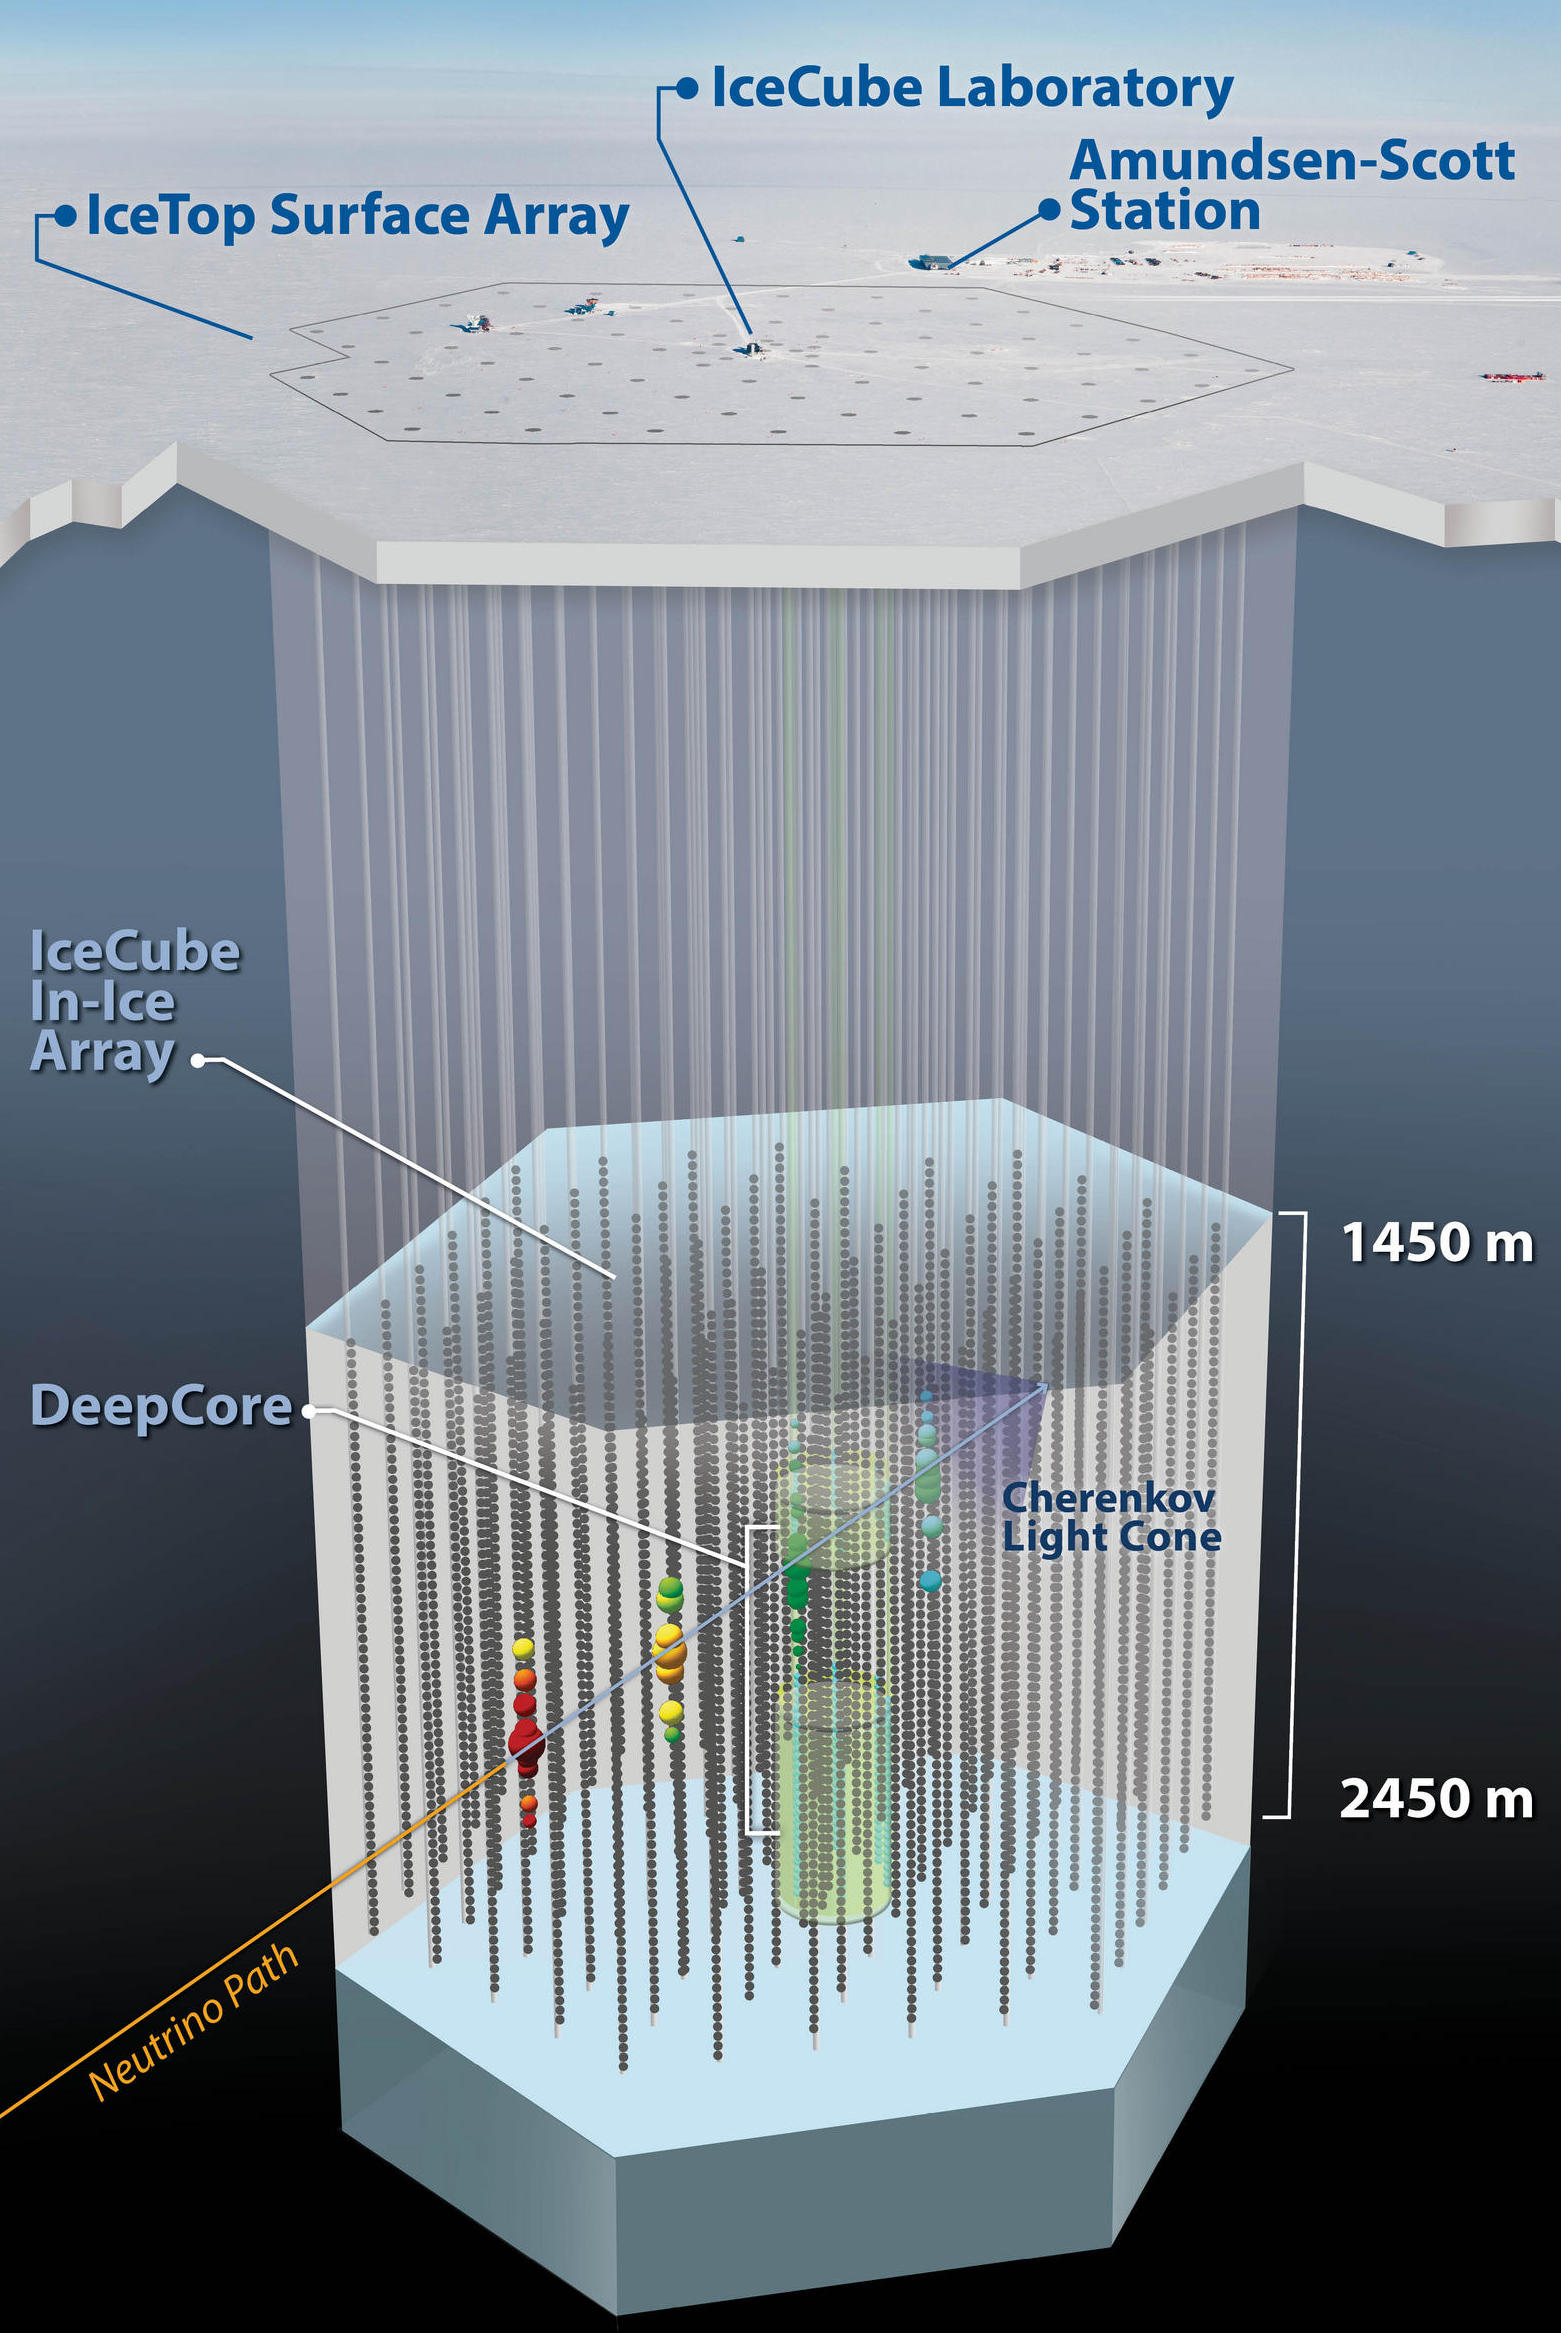
\includegraphics[width=\textwidth]{./images/icecube_detector.jpg}
        \caption{Sketch of the IceCube facilities at the South Pole and how an event view of a muon neutrino could look like. \cite{IceCubePics}}
        \label{fig:icecube_detector}
    \end{subfigure}
    \hfill
    \begin{subfigure}[t]{0.38\textwidth}
        \centering
        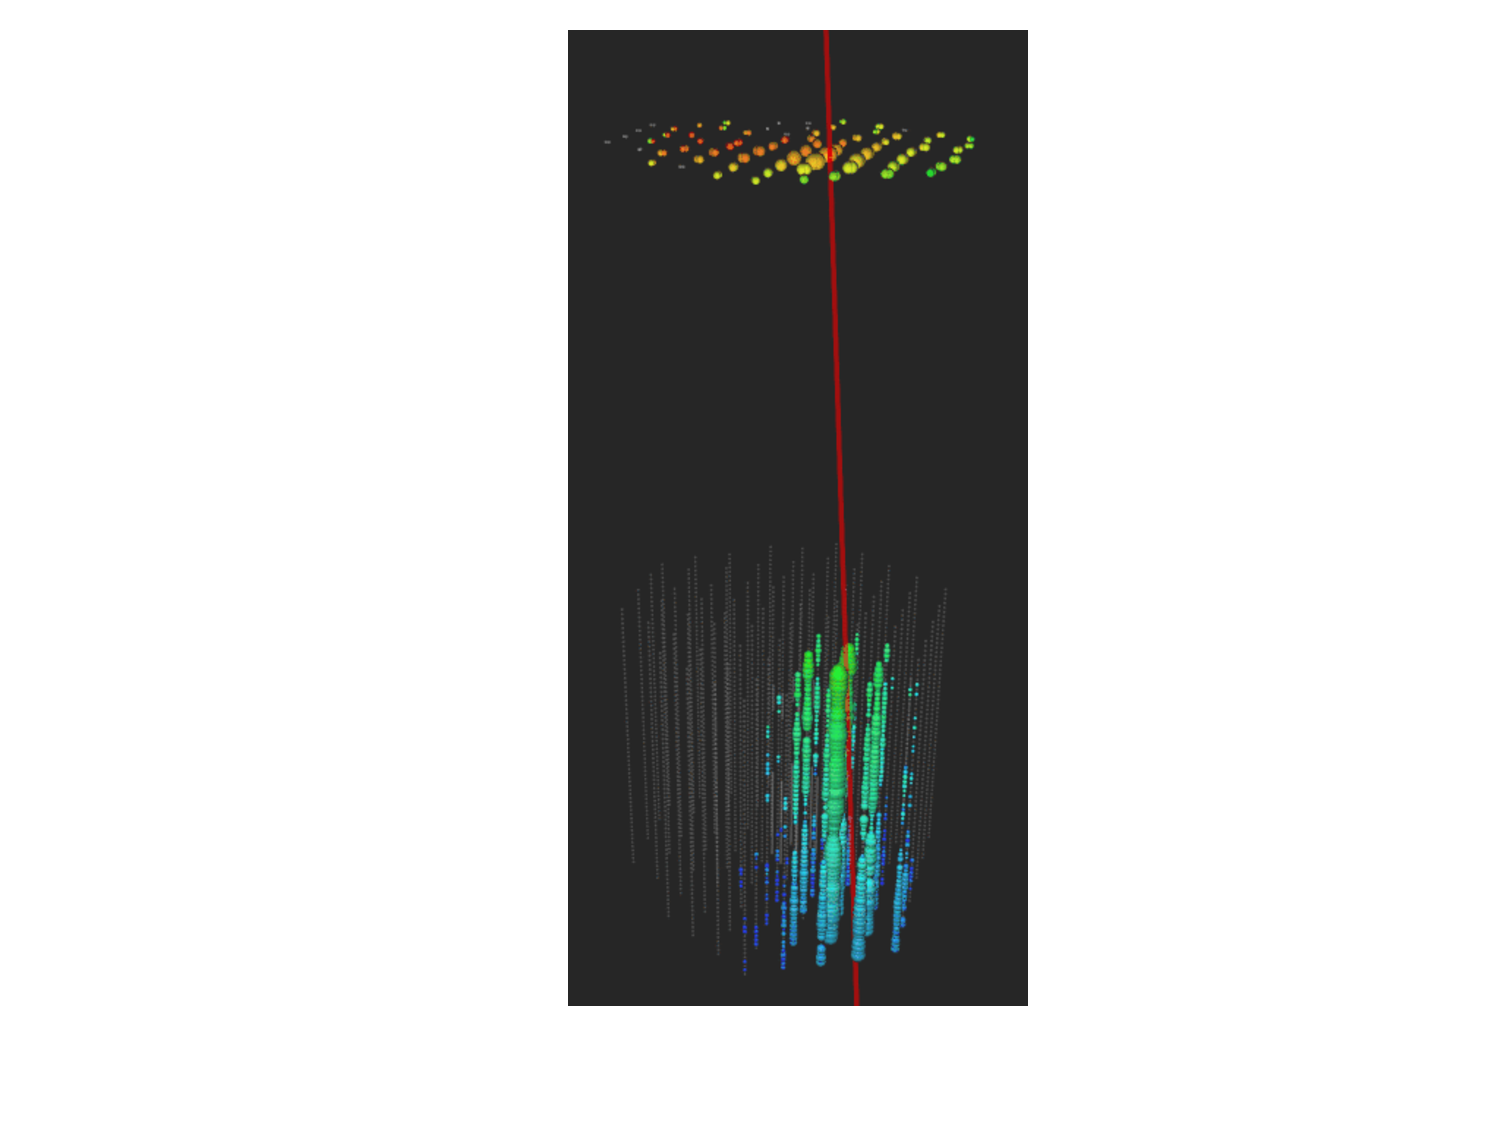
\includegraphics[width=\textwidth]{./images/icecube_event_300_pev_2010_07_02.pdf}
        \caption{Event view of a measured cosmic ray event in IceTop and IceCube on 02.07.2010 with a reconstructed primary particle energy of \SI{300}{PeV}. \cite{IceCubePics}}
        \label{fig:icecube_event_view}
    \end{subfigure}
    \caption{The IceCube Neutrino Observatory including the IceTop Array at the surface, the main in-ice detector and the DeepCore extension. For the event views, each colored circle indicates a DOM that measured light. The color ranges represents the time from red, early to blue, late. The size of the DOMs scales with the amount of detected light.}
    \label{fig:icecube}
\end{figure}

In the middle of IceCube 8 Strings, each with 60 DOMs of higher quantum efficiency are placed more densely together.
This extension called \enquote{DeepCore} decreases the lower threshold for neutrino energies to \SI{10}{GeV} and uses the rest of IceCube as a veto region.
Another extension is \enquote{IceTop} where a water Cherenkov tank is placed at the surface of each string.
This can either be used as an air shower detector at an altitude of \SI{3}{km} with the benefit of IceCube as a further muon detector to deeper analyze the atmospheric muons.
On the other side, it works as a veto for IceCube to distinguish down-going neutrinos from atmospheric muon events as the neutrinos should not be seen in IceTop.

There are currently plans for an extension of IceCube named IceCube-Gen2 \cite{IceCube20Gen2}.
The planned detector is shown in \figref{fig:detect_gen2}.
An extension called \enquote{IceCube-Upgrade} has already been funded to test new types of DOMs for Gen2.
Gen2 will enlarge the detected volume to \SI{8}{\cubic\kilo\meter} and will be placed around IceCube.
In contrast to IceCube, the Strings in Gen2 will be organized on a sunflower structure avoiding corridors where muons can sneak inside the inner volume and mimic a starting event.
Besides, a radio detector is planned, placing the antennas on a grid with an inner distance of a kilometer covering an area of \SI{100}{\cubic\kilo\meter} to analyze the cosmogenic neutrinos.
\begin{figure}
    \centering
    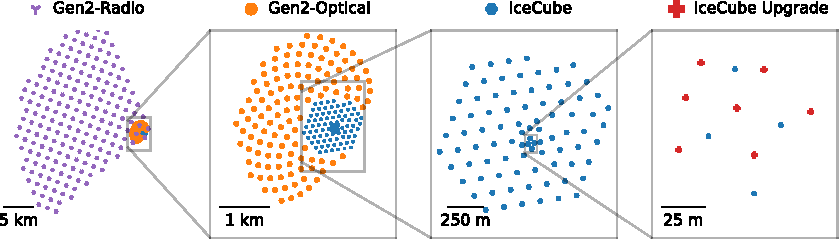
\includegraphics[width=\textwidth]{./images/detector_gen2.pdf}
    \caption{Schematic top view of the IceCube detector compared to the enhancements for Gen2. \cite{IceCube20Gen2}}
    \label{fig:detect_gen2}
\end{figure}

A distinct astrophysical neutrino source has also not been measured yet as well as a class of sources in a stacked search \cite{IceCube20PointSource, IceCube17BlazarStacking}.
However, a coincidence of a high energy neutrino event originating from the same direction as an AGN flaring at the same time in the gamma energy region is the first hint of a possible neutrino source \cite{IceCube18MMA, IceCube18TXS}.

\subsubsection{Event Signatures}

The measured event signatures are mainly divided into tracks and cascades.
A long track signature of an atmospheric muon bundle is shown in \figref{fig:icecube_event_view}.
Tracks are long, nearly straight lines along the muon path with the energy losses along the track producing the track signature.
Due to their long range, they can be further classified into starting, stopping, through-going and corner clippers.
Only neutrinos can produce starting events and stopping events can only be produced by a huge stochastic loss, which happens rarely or by low energetic muons.
Most-often, muons propagate through the detector producing a long path along their track.
There is however the special case of a corner clipper, that can mimic a cascade-like event at the edge of the detector.

A particle shower created by a single particle interaction (or multiple interactions inside a small range of less than \SI{10}{m}, which is pint-like for IceCube), produces a rather spherical spread of the produced Cherenkov light.
Although the particle cascade is boosted in the forward direction with just small transversal momentum and a Moli\`{e}re radius in the ice of \SI{10}{cm} \cite{PDG20}, the small scattering length creates a spherical propagation of the produced Cherenkov light.

NC-interactions of all neutrino flavors have just a visible hadronic shower, as the incoming and outgoing neutrino doesn't produce a signal, thus producing a single cascade.
Regarding CC interactions and starting with the electron neutrino, the additional electron loses most of its energy in less than \SI{10}{m} in the ice.
As this distance is point-like for IceCube, the resulting cascade also has a spherical structure.
Although there are differences in the shower developments of electromagnetic and hadronic cascades, especially through the later decays of neutral hadrons, it was not possible yet to distinguish between electromagnetic and hadronic cascades \cite{Steuer17ICRC}.

The greater mass of muons compared to electrons makes them lose their energy much slower and let them travel several kilometers through the ice.
From the hadronic cascade at the neutrino interaction vertex, a long track is going out.
Therefore muon neutrinos do not have to interact inside the detection volume and can also interact far before the detector with the muons traveling inside, increasing the effective detector volume.
\begin{figure}
    \centering
    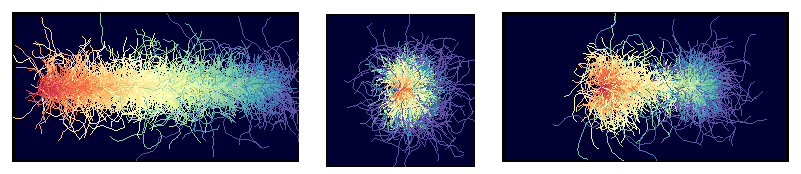
\includegraphics[width=\textwidth]{./images/icecube_sim_event_signatures.pdf}
    \caption{Simulated paths of the produced Cherenkov photons for the three major event signatures of a through-going muon (left) an electron neutrino (middle) and a tau neutrino (right). The color represents the time from red (early) to blue (late). \cite{IceCube18Sim}}
    \label{fig:icecube_event_signatures}
\end{figure}

Tau leptons have an even higher mass compared to the muons and have therefore a smaller energy loss resulting in a thin propagation track.
But the small lifetime of \SI{290}{fs} makes them decay directly or for higher energies let them just travel \SI{50}{m} per PeV.
The event signature depends on the decay channel; two-thirds are the hadronic decay channel and the last third is equally distributed between the muonic and the electronic channel.
Until energies of around \SI{10}{TeV} the second hadronic or em-cascade can not be distinguished from the first hadronic cascade at the neutrino vertex.
For higher energies first, a double pulse waveform at a single DOM can be registered and later these two cascades get separated more clearly and a double cascade or double bang signature is created.
These three major event signatures are shown in \figref{fig:icecube_event_signatures}.

The muonic tau decay also contributes to the amount of incoming muons starting before the detector.
For events starting inside the detector, the outgoing track is smaller compared to the hadronic cascade as the additional neutrinos from the tau decay take away some energy.
For higher energies, the thin tau track goes over to a brighter muon track.
But these differences in the track signature can just be separated statistically for many events and not on an event level due to the stochasticity of the propagation.
Due to the limited resolution, there has been just one promising tau neutrino event seen with IceCube after 10 years of measurement \cite{Meier19ICRC, IceCube20HeseTau}.

\subsubsection{Event selections}

The main interesting features to be reconstructed are the primary particle type, its energy and the direction.
To extract the primary particle type a classification of the different event signatures is required.
For these selections, multivariate methods are required since the atmospheric muon rate of \SI{1}{kHz}, is many orders above the atmospheric neutrino rate of \SI{1}{mHz} or the astrophysical neutrino rate of \SI{1}{\micro.Hz}.

A pure \textbf{cascade sample} contains mostly CC interacting electron neutrinos, fewer NC events and a few tau neutrinos.
Cascade searches \cite{IceCube20Cascades} uses the outer DOM layers as veto region against through-going muons, which have a detection rate that is multiple orders of magnitudes higher.
But even in DeepCore, muon tracks are contaminating the cascaded selections when traveling in the middle between the strings due to the lattice structure.
Also, the stochasticity of the propagation processes, allowing muons to travel without visible losses and then deposit all of their energy in a catastrophic loss inside the detector limits the selection efficiency.
As these processes are rare, an accurate description of the muon physics even at the tails or edges of the total and differential cross section is needed.
These selection methods are not just valid for cascades, but all kind of starting events.

The tracks are further separated between up-going and down-going tracks.
Down-going events are most-often atmospheric muons reaching the detector as bundles with a lateral distance of some meter between them.
Those events are seen as one thick, bright track due to the limited resolution preventing a separation of the single muons from a bundle.
Therefore those muon bundles are in principle of limited usefulness since the number of muons and their energy is not reconstructible.
An approach to analyzing atmospheric muon bundles is the search for a \textbf{leading muon} containing most of the bundle energy \cite{Fuchs16PhD, Fuchs16ECRS, Werthebach17Master}.
A bundle of many low energetic muons creates a bright track with a continuous energy loss.
Leading or single muons have higher stochasticity, e.g. with a huge bremsstrahlung loss resulting in a thinner track with brighter cascades along it.
As these muons are produced in one of the first interactions of the air shower they can provide further insights into the particle processes in the atmosphere.

Another approach to use atmospheric muons is using \textbf{stopping muons} \cite{Hoinka17Master, Ninfa19Master}.
They are most-often single muons and have energies of just several \SI{100}{GeV} when entering the detector.
At these energies, they are in the regime of the minimal Ionization and can be used to calibrate the detector and measure systematic parameters.
For stopping muons, also the range they have traveled through the ice is known which is an approximation of their energy at the surface.
Therefore they can also be used to study cosmic ray and air shower physics, but in comparison to the leading muons for higher energies, stopping muons provide insights at lower energies.

\textbf{Up-going muon tracks} can only be neutrino-induced muons as muons cannot propagate large distances through the earth.
Unfortunately, a simple extraction of these muons with a zenith cut is not satisfying as the resulting sample is still dominated by mis-reconstructed muons.
Although the directional resolution is high for tracks, sometimes it can exceed \SI{5}{\degree} and contaminate the sample.
Therefore advanced machine learning algorithms are used to extract a purified sample \cite{Stettner19ICRC}.
The filtered track events are an ideal single muons sample at all energies; good to analyze the muon physics, e.g. the energy loss profile.
Just for the starting events, the hadronic cascade of the neutrino interaction contaminates a little bit.

\subsubsection{Event Reconstruction}

After the selection, the energy and directional reconstruction is the remaining step before analyzing the desired event sample.
An overview of the standard reconstruction methods is given in \cite{AMANDA2004Reco, IceCube2014Ereco}.
In recent years also modern, machine-learning-based methods using e.g. Deep Neural Networks have been developed increasing the accuracy of the reconstruction \cite{Huennefeld17ICRC, Huennefeld17Master, Huennefeld19VLVNT, IceCube20DNN}.
A comparison of the standard and neural network approaches for the reconstructions is shown in \figref{fig:icecube_reco} as well as their energy dependence.
\begin{figure}
    \centering
    \begin{subfigure}{0.55\textwidth}
        \centering
        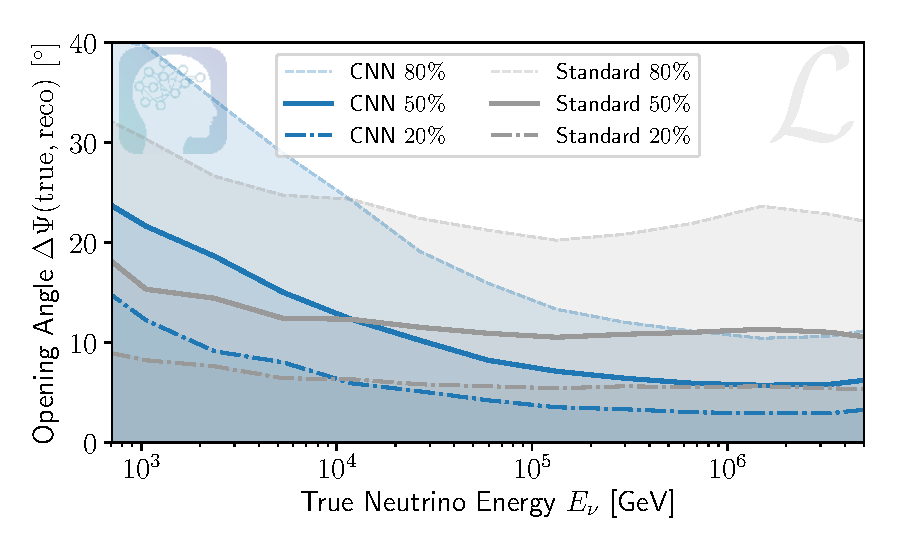
\includegraphics[width=\textwidth]{./images/icecube_resolution_cascade_angular.pdf}
        \caption{Resolution of the angular reconstruction for cascades comparing the standard likelihood approach with a Neural Network (CNN). \cite{IceCube20DNN}}
        \label{fig:icecube_angular_resolution}
    \end{subfigure}
    \hfill
    \begin{subfigure}{0.43\textwidth}
        \centering
        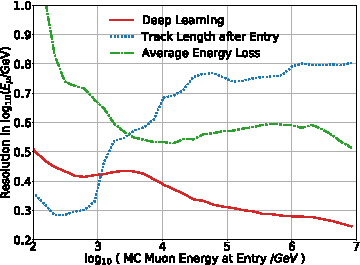
\includegraphics[width=\textwidth]{./images/icecube_resolution_muon_energy.pdf}
        \caption{Resolution of the energy reconstruction for tracks comparing the standard $\mathrm{d}E/\mathrm{d}X$ and track length approach with a Deep Neural Network. \cite{Huennefeld17Master}}
        \label{fig:icecube_energy_resolution}
    \end{subfigure}
    \caption{Energy dependence of the resolution of the challenging reconstruction parameters in IceCube. On the left the angular reconstruction for cascades and on the right the energy reconstruction for tracks is compared between modern neural network approaches and the default likelihood approaches.}
    \label{fig:icecube_reco}
\end{figure}

The directional resolution for tracks is comparably high (\SI{0.5}{\degree}) while being low for cascade events (\SI{15}{\degree}).
Regarding the energy reconstruction, it's the other way round.
When a cascade is contained inside the detector the energy resolution is high due to the calorimetric measurement resulting in an uncertainty of \SI{10}{\%}.
For through-going tracks, just a portion of the muon energy loss is deposited inside the detector
For muons above a TeV the energy is reconstructed using the average energy loss per distance $\mathrm{d}E/\mathrm{d}X$, which increases nearly linear with the muon energy (c.f. section \ref{sec:dedx}).
Therefore, the track inside the detector is split into multiple segments and the high energetic, stochastic losses are cut away to extract the continuous energy loss.
Since the linear dependency of the average energy loss on the muon energy starts at around a TeV, while being independent for lower energies, this can only be applied at energies above a TeV.
For starting tracks, the energy resolution of the muons and neutrinos improves, due to the additional information of the hadronic cascade at the vertex.
For low energy muons, the average energy loss is not proportional to the muon energy.
As these muons are most-often stopping inside the detector, the track length can be used to reconstruct the energy.

Next to the energy and direction, also the energy losses along a muon track can be reconstructed, which is important for analyses depending on the stochasticity, e.g. when creating a leading muon sample.
Since IceCube cannot distinguish between single energy losses, the track inside the detector is split into multiple segments as for the $\mathrm{d}E/\mathrm{d}X$ energy reconstruction and the energy loss in each segment unfolded.
This is just sensitive to high stochastic energy losses and can be used to study the energy loss profile of the muons.

\subsubsection{Systematic Uncertainties}

The remaining task, an analysis has to consider, are systematic uncertainties.
In every experiment, some remaining parameters are challenging to calibrate or measure and have uncertainties that are non-negligible for analyses.
For the IceCube detector, one main systematic parameter is the quantum efficiency of the DOMs, short DOM efficiency.
This varies the amount of detected light and has an uncertainty of $\pm\SI{5}{\percent}$.
However, in this factor multiple uncertainties are combined, all scaling the amount of detected photons and which cannot be distinguished from each other.
Also cross-section uncertainties may be an origin, why this factor is not equal to 1.

The other main uncertainties are the ice properties, mainly the absorption and scattering lengths, which are depth-dependent.
The depth dependence does not originate due to the different levels of pressure and thus temperature, but due to several layers of dust \cite{Icecube06ice, Icecube13ice}.
Especially in the middle of the detector at a depth around \SI{2}{km} the absorption length is significantly decreased and nearly all photons get absorbed before reaching a DOM.
This blind layer is slightly indicated in \figref{fig:icecube_event_view}.
Further systematics of the glacial ice like the anisotropy are discussed in detail in \cite{Rongen19PhD}.

Next to these detector and ice properties, further sub-dominant systematics arise due to the theoretical uncertainties of the physical processes.
Regarding the muon physics, the uncertainties of the cross sections needs to be differentiated between the processes dominant for the low energy losses and processes dominating the high, stochastic energy losses.
While an increase of the low energy losses can already be compensated by an increase in the DOM efficiency, the uncertainties of the stochastic energy losses have not been considered, yet.
Since the stochasticity of the muon affects the performances of separating leading muon, cascade or tau samples, an approach to include them is analyzed in this work.

One of the largest systematic uncertainties is the flux of atmospheric neutrinos, which is often the limiting factor for the sensitivity of analysis.
This can be avoided using e.g. an unfolding approach, which is independent of the flux model used in the simulations.
However, if this is not feasible, the uncertainty of the flux needs to be taken into account, e.g. by using the so-called Barr parameters \cite{Barr06}.

To take into account all of these systematics, simulation sets each varying one or two systematic parameters on a grid and interpolations between these grid points were used in analyses.
However, this grid approach increases the number of required simulation sets for every further systematic parameter resulting in the curse of dimensionality.
There is now a new approach \cite{IceCube2019SnowStorm} where for each simulation run a new set of all systematic parameters is sampled from their uncertainty distribution, including correlation.
With this Monte-Carlo approach, the phase space can be filled also when including further systematics.

% \chapter{Muon Interaction} \label{sec:interactions}

The muon cross-sections described in this chapter focus on muons above a GeV and the relevant processes for the simulation of astroparticle experiments.
These processes are all included in the simulation library PROPOSAL or are intended to be included in the future.
In principle, they are also valid for the other charged leptons, electrons, and taus, if not stated differently.
% At least at high energies the deviations due to interferences or the different mass vanishes.

All cross-sections $\sigma$ are differential in the energy loss $v$ relative to the energy of the primary particle $E$, given as $\dif \sigma / \dif v$ or as the average energy loss over distance $X$
\begin{align} \label{eq:dedx_int}
    \left\langle - \frac{\dif E}{\dif X} \right\rangle = \frac{N_A}{A} \int v \frac{\dif \sigma}{\dif v} \dif v.
\end{align}
The cross-sections are also given in a generalized form for particles with mass $M$ and charge $z$.
Mainly the natural unit system is used with the symbolic definitions listed in \tabref{tab:symbols}.
\begin{table}
    \centering
    \caption{Definitions of the symbols used in this thesis, unless stated otherwise or mentioned explicitly.}
    \label{tab:symbols}
    \begin{tabular}{cl}
        \toprule
        Symbol & Definition \\
        \midrule
        $c_0$ & Speed of light in vacuum ($=1$ in n.u. and $\approx \SI{3e8}{m.\per.s}$ in SI units) \\
        $N_A$ & Avogadro constant ($\approx \SI{6e23}{\per.\mol}$) \\
        $\alpha$ & Fine structure constant ($\approx 1/137$) \\
        $m_{e,\mu,\dots}$ & Mass of a particle with the lower index defining the particle type \\
        $r_{e (\mu)}$ & Classical electron (muon) radius ($r_e\approx \SI{2.8}{fm}, r_\mu = r_e \sfrac{m_e}{m_\mu}$) \\
        $E, p$ & Energy and momentum of a particle with $E^2 = p^2 + m^2$\\
        $\beta$, $\gamma$ & Lorentz factors in relativistic approximation, $\beta = p/E$ and  $\gamma = E/m$ \\
        $M, z$ & Mass and charge of the primary particle to propagate \\
        $Z, A$ & Number of protons (nucleons) in the target nucleus \\
        $K$ & Ionization constant $4\pi N_A r_e^2 m_e \approx \SI{0.3}{MeV.cm^2 / mol}$ \\
        $X_0$ & Radiation length of a medium (c.f. \ref{sec:medium}) \\
        $q, Q^2$ & 4-momentum of the virtual photon exchanged with a nucleus \\
        $B_{\text{(in)el}}$ & (in)elastic radiation logarithm constant of the screening (section \ref{sec:medium}) \\
        \bottomrule
    \end{tabular}
\end{table}

An overview of the energy loss of muons is shown in \figref{fig:dedx_pdg} which is divided into four areas in energy.
At the lowest energies ($\beta < \alpha$) the velocity of the muons is smaller than the velocity of the valence electrons.
Non-ionizing losses mainly driven by nuclear recoil are the main process for $\beta \ll \alpha$ before ionizing energy losses increase proportionally to the velocity of the muon \cite{Groom01}.
The energy region between $\alpha < \beta < \num{0.1}$ is not yet theoretically well understood and only empirical models are used to describe these energy losses \cite{Groom01}.
For both low energy regions, the data in \figref{fig:dedx_pdg} are taken from pion and proton tables in \cite{ICRU49} and scaled according to the mass ratios to the muon.
Both regions also differ between $\mu^+$ and $\mu^-$ since the latter is likely to get captured into atomic orbitals, quickly cascading down into the 1s orbital and then decay or weakly interact with the nucleus (c.f. \cite{Measday01}).

For $\beta > \num{0.1}$, the ionization and excitation losses are well described by the Bethe-Bloch theory.
The energy loss decreases to a minimum ionization point, a characteristic energy for a medium at around a GeV before it starts increasing logarithmically with the energy.
The radiative losses, i.e. bremsstrahlung, pair production, and inelastic nuclear interaction, increase linearly with the energy surpassing the ionization losses at a TeV and dominating the energy loss at high energies.
Initially, the inelastic nuclear interaction is just a \SI{10}{\%} correction compared to the other two processes, but increases slightly quicker and surpassing the other two even before the LPM-effect limits them, which occur between PeV and ZeV energies and is therefore not included in \figref{fig:dedx_pdg}.
\begin{figure}
    \centering
    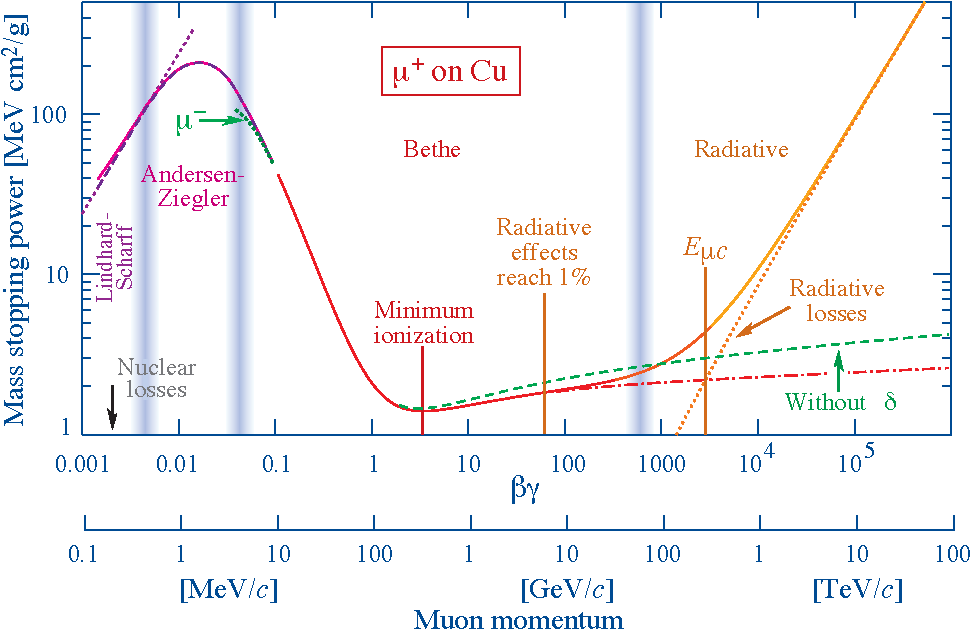
\includegraphics[width=0.82\textwidth]{./images/muon_dedx_pdg.pdf}
    \caption{Average energy loss of muons in copper. \cite{PDG20}}
    \label{fig:dedx_pdg}
\end{figure}

%
% new section
%

\section{The average Energy Loss} \label{sec:dedx}

At energies above a GeV, muons lose their energy via four main interaction types, ionization, $e^+e^-$ pair production, bremsstrahlung, and inelastic nuclear interactions, which is often referred to as photonuclear interaction.
While the ionization is nearly constant and just increases logarithmically with the energy, the other three processes increase linearly with the energy surpassing the Ionization at around a TeV, depending on the medium.
This behavior can be visualized in the average energy loss in \figref{fig:dedx_pdg}.
Besides the four main interactions, there are further processes with just minor influence on the energy loss, but also important for the muon propagation, the $\mu^+\mu^-$ pair production, and the weak interaction.
Regarding the decay, the muons have a relatively long lifetime of around \SI{2.2}{\micro\second} \cite{PDG20}.
They usually lose nearly all of their energy, slow down that the $\mu^-$ even get absorbed by an atom and decay with a total energy of almost their rest mass.
Therefore, the decay process does also not contribute to the energy loss as indicated in \figref{fig:dedx_all}.

As the weak interaction and the decay are purely stochastic processes and have no continuous energy loss, their contribution in \figref{fig:dedx_all} is adapted.
For both the decay and the weak interaction, the average energy loss is indicated by multiplying the energy times the total cross-section.
Using the mean lifetime $\tau$, the cross-section for the decay is defined by
\begin{align} \label{eq:sigma_decay}
    \sigma_{\text{decay}} = \frac{1}{\beta \gamma \tau c_0}.
\end{align}
The sum of the energy loss can be parameterized using a quasi-linear approximation
\begin{align} \label{eq:dedx_approx}
    \left\langle - \frac{\dif E}{\dif X} \right\rangle = a(E) + b(E) \cdot E.
\end{align}
Thereby, the functions $a$ and $b$ only depend logarithmically on the energy, while $a$ is mainly defined by the Ionization and $b$ by the three radiative processes.

Assuming $a$ and $b$ as constant values, the average range of the muons can be approximated by
\begin{align} \label{eq:dedx_range}
    R_{\left\langle \frac{\dif E}{\dif X} \right\rangle} = \frac{1}{b} \logn \left( 1 + \frac{b}{a} E \right).
\end{align}
This simple linear model, shown in \figref{fig:dedx_range}, already provides a rough description of the muon energy loss and range and is used in many applications as a first estimation of the muon contribution.
A comparison with more precise calculations of the range using Monte-Carlo techniques is shown in \figref{fig:prop_range}.
\begin{figure}
    \centering
    \begin{subfigure}{0.9\textwidth}
        \centering
        \includegraphics[width=\textwidth]{./plots/dedx_all.pdf}
        \caption{The average energy loss of muons.}
        \label{fig:dedx_all}
        \vspace{0.5cm}
    \end{subfigure}
    \begin{subfigure}{0.9\textwidth}
        \centering
        \includegraphics[width=\textwidth]{./plots/dedx_range.pdf}
        \caption{The average range of muons using the $\dif E / \dif X$ fit.}
        \label{fig:dedx_range}
    \end{subfigure}
    \caption{The average energy loss and range of muons in Standard Rock ($Z=11, A=22$) using the linear approximation in \ref{eq:dedx_approx}. The fitted values are then used to calculate the average range given by \ref{eq:dedx_range}. The contribution of the decay and the weak interaction to the \enquote{continuous energy loss} is described in the text.}
    \label{fig:dedx}
\end{figure}

%
% new section
%

\section{Ionization} \label{sec:ioniz}

The ionization describes the release of an electron from the atomic shell, producing an ion.
Regarding the muon cross-sections, the excitation of an atom and the scattering at atomic electrons are included in the wider meaning of Ionization.
In contrast to all other interactions, the ionization is given as differential cross-section, but also in the average energy loss, since the density effect can only be included in the average energy loss.

The differential cross-section describing the knock-on electrons was mainly derived by Bethe \cite{Bethe30} and combined with further corrections into an expression by Rossi \cite{Rossi52}.
\begin{align} \label{eq:ioniz_dsigma}
\frac{\dif \sigma}{\dif v} = 
    \frac{1}{2} K z^2 \frac{Z}{A} \frac{1}{(\beta Ev)^2}
    \left[ 1 - \beta^2 \frac{v}{v_{\text{max}}} + \frac{1}{2} \left( \frac{v}{1 + 1/\gamma} \right)^2
    \right]
\end{align}
The $1/v^2$ dependency already indicates that this cross-section is responsible for the lower energy losses.
The maximum energy transferred to the electrons is given by \cite{PDG20}
\begin{align} \label{eq:ioniz_vmax}
    E v_{\text{max}} = \frac{2 m_e \beta^2 \gamma^2}{1 + 2 \gamma \frac{m_e}{M} + \left(\frac{m_e}{M}\right)^2},
\end{align}
which is an analytic interpolation between the approximations of the extreme scenarios at low and high energies
\begin{align}
    Ev_{\text{max}} =
    \begin{cases} 
        2m_e\beta^2 \gamma^2, & \text{ for } 2\gamma m_e \ll M \\
        M \beta^2 \gamma & \text{ for } 2\gamma m_e \gg M.
    \end{cases}
\end{align}
According to \eqref{eq:dedx_int} the average energy loss is obtained by integrating \eqref{eq:ioniz_dsigma} between
\begin{align}
    v_{\text{min}} = \frac{1}{2m_eE} \left( \frac{I_{\text{excit.}}}{\beta\gamma} \right)^2,
\end{align}
and a $v_{\text{up}}$ located between the limits.
Including the correction of the density effect $\delta$, this results in
\begin{align}
\frac{\dif E}{\dif X} = z^2 \frac{Z}{A} \frac{K}{2\beta^2}
    \left[
        \logn \frac{2 m_e \beta^2 \gamma^2 Ev_{\text{up}}}{I_{\text{excit.}}^2}
        - \beta^2 \left( 1 + \frac{v_{\text{up}}}{v_{\text{max}}} \right)
        + \left( \frac{v_\text{up}}{2(1 + 1/\gamma)} \right)^2
        - \delta
    \right]
\end{align}
with $I_{\text{excit.}}$ the mean excitation energy of the medium.
The reason for integrating to $v_{\text{up}}$ instead of $v_{\text{max}}$ is due to the energy loss cut, described in section \ref{sec:ecuts}, that is necessary for the simulations.

The density effect describes the reduction of the ionization due to the polarisation of the medium, which has an increasing effect at higher energies, indicated in \figref{fig:dedx_pdg}.
This is not included in the differential cross-section as it is a purely continuous energy loss process and not a stochastic interaction.
Depending on the energy parameter $x = \log_{10}(\beta\gamma)$, it is parameterized in \cite{Sternheimer52}
\begin{align}
\delta =
    \begin{cases}
        \delta_0 10^{2(x - x_0)}, & \text{ for } x < x_0\\
        2 \logn 10 x + c + a(x_1 - x)^b, & \text{ for } x_0 \leq x \leq x_1 \\
        2 \logn 10 x + c & \text{ for } x_1 \leq x
    \end{cases}
\end{align}
The density constants $\delta_0, x_0, x_1, a, b, c$ as well as the excitation energy $I_{\text{excit.}}$ are specific constants for each medium and defined in \cite{Groom01}.
For selected media that are implemented in PROPOSAl, these constants are listed in \tabref{tab:ioniz_const}.
\begin{table}
    \caption{The excitation energy and further density correction parameters for selected media mainly used in PROPOSAL. \cite{Groom01}}
    \label{tab:ioniz_const}
    \begin{center}
    \begin{tabular}{l | S[table-format=3.1] S[table-format=+1.4] S[table-format=1.4] S[table-format=1.5] S[table-format=1.4] S[table-format=2.4] S[table-format=1.2]}
        \toprule
        Medium & {$I_{\text{excit.}}$} & {$x_0$} & {$x_1$} & {$a$} & {$b$} & {$-c$} & {$\delta_0$} \\
        \midrule
        Air           & 85.7  & 1.7418 & 4.2759 & 0.10914 & 3.3994 & 10.5961 & 0 \\
        Water         & 79.7  & 0.2400 & 2.9004 & 0.09116 & 3.4773 & 3.5017 & 0 \\
        Ice           & 79.7  & 0.2586 & 2.8190 & 0.09116 & 3.4773 & 3.5873 & 0 \\
        Standard Rock & 136.4 & 0.0492 & 3.0549 & 0.08301 & 3.4120 & 3.7738 & 0 \\
        Iron          & 286.0 & -0.0012 & 3.1531 & 0.14680 & 2.9632 & 4.2911 & 0.12 \\
        Uranium       & 890.0 & 0.2260 & 3.3721 & 0.19677 & 2.8171 & 5.8694 & 0.14 \\
        \bottomrule
    \end{tabular}
    \end{center}
\end{table}

The inelastic bremsstrahlung on atomic electrons when the atomic electron emits the bremsstrahlung, described in section \ref{sec:brems_inel}, is most often considered as an ionization loss since the atom also gets ionized.
While the main bremsstrahlung cross-section has an energy loss behavior of $1/v$ the so-called $e$-diagrams (see the Feynman diagram in \figref{fig:feyn_brems_e}) have a sharp energy loss spectrum of $1/v^2$, shown in \eqref{eq:brems_e_diagram}, similar to ionization.

The differential cross section of the ionization processes is shown in \figref{fig:ioniz_dsigma} mainly showing the $1/v^2$ dependency and a flattening of the $e$-diagram bremsstrahlung to small energy losses due to the parametrization.
In \figref{fig:ioniz_dedx} the average energy loss of the two contributions and the additional density correction are shown.
\begin{figure}
    \centering
    \begin{subfigure}{0.9\textwidth}
        \centering
        \includegraphics[width=\textwidth]{./plots/ioniz_dsigma.pdf}
        \caption{The differential cross section of the ionization processes at \SI{1}{TeV}.}
        \label{fig:ioniz_dsigma}
        \vspace{0.5cm}
    \end{subfigure}
    \begin{subfigure}{0.9\textwidth}
        \centering
        \includegraphics[width=\textwidth]{./plots/ioniz_dedx.pdf}
        \caption{The average energy loss of the ionization processes.}
        \label{fig:ioniz_dedx}
    \end{subfigure}
    \caption{The Ionization cross-section of muons in Standard Rock ($Z=11, A=22$). The Bethe-Bloch term is compared to the inelastic interaction on atomic electrons with the electrons emitting a bremsstrahlung photon ($e$-diagram) and the negative contribution of the density correction.}
    \label{fig:ioniz}
\end{figure}

%
% new section
%

\section{Bremsstrahlung} \label{sec:brems}

The Bremsstrahlung process, where the muon emits a photon and exchanges the remaining momentum with a nucleus in an elastic process, can be visualized in the Feynman diagrams in \figref{fig:feyn_brems}.
\begin{figure}
    \centering
    %
\begin{tikzpicture}
\begin{feynman}
    % define vertices
    % muon
    \vertex (mu_in) at (-\feynlen-\feynsmallen, 0);
    \vertex[right=2.5*\feynlen of mu_in] (mu_out);
    \vertex[right=\feynlen of mu_in] (mu_vertex_nucl);
    \vertex[left=\feynlen of mu_out] (mu_vertex_brems);
    % brems
    \vertex[above=\feynlen of mu_out] (brems_out);
    % nucleus
    \vertex[below=\feynlen of mu_in] (n_in);
    \vertex[below=\feynlen of mu_vertex_nucl] (n_vertex);
    \vertex[below=\feynlen of mu_out] (n_out);
    % draw diagram
    \diagram* {
        (mu_in) -- [fermion] (mu_vertex_nucl) -- (mu_vertex_brems) -- [fermion] (mu_out),
        (mu_vertex_nucl) -- [boson] (n_vertex),
        (mu_vertex_brems) -- [boson] (brems_out)
    };
    % draw extra features with tikz (not available in tikz-feynman)
    \draw[thick, double] (n_in) -- (n_vertex) -- (n_out);
    \draw[fill] (n_vertex) circle[radius=\feynvertexsize];
    \draw[fill] (mu_vertex_nucl) circle[radius=\feynvertexsize];
    \draw[fill] (mu_vertex_brems) circle[radius=\feynvertexsize];
    % add labels
    \node[left] at (mu_in) {$\mu$};
    \node[right] at (mu_out) {$\mu '$};
    \node[right] at (brems_out) {$\gamma$};
    \node[left] at (n_in) {$N$};
    \node[right] at (n_out) {$N'$};
\end{feynman}
\end{tikzpicture}
%
\hspace{1cm}
%
\begin{tikzpicture}
\begin{feynman}
    % define vertices
    % muon
    \vertex (mu_in) at (-\feynlen-\feynsmallen, 0);
    \vertex[right=2.5*\feynlen of mu_in] (mu_out);
    \vertex[left=\feynlen of mu_out] (mu_vertex_nucl);
    \vertex[right=\feynlen of mu_in] (mu_vertex_brems);
    % brems
    \vertex[above=\feynlen of mu_out] (brems_out);
    % nucleus
    \vertex[below=\feynlen of mu_in] (n_in);
    \vertex[below=\feynlen of mu_vertex_nucl] (n_vertex);
    \vertex[below=\feynlen of mu_out] (n_out);
    % draw diagram
    \diagram* {
        (mu_in) -- [fermion] (mu_vertex_brems) -- (mu_vertex_nucl) -- [fermion] (mu_out),
        (mu_vertex_nucl) -- [boson] (n_vertex),
        (mu_vertex_brems) -- [boson] (brems_out)
    };
    % draw extra features with tikz (not available in tikz-feynman)
    \draw[thick, double] (n_in) -- (n_vertex) -- (n_out);
    \draw[fill] (n_vertex) circle[radius=\feynvertexsize];
    \draw[fill] (mu_vertex_nucl) circle[radius=\feynvertexsize];
    \draw[fill] (mu_vertex_brems) circle[radius=\feynvertexsize];
    % add labels
    \node[left] at (mu_in) {$\mu$};
    \node[right] at (mu_out) {$\mu '$};
    \node[right] at (brems_out) {$\gamma$};
    \node[left] at (n_in) {$N$};
    \node[right] at (n_out) {$N'$};
\end{feynman}
\end{tikzpicture}
%
    \caption{The two Feynman diagrams of a muon emitting a Bremsstrahlung photon and exchange a momentum with a nucleus are shown, differing in the order when the photon to the nucleus and the bremsstrahlung photon couples to the muon line.}
    \label{fig:feyn_brems}
\end{figure}

A general expression of the cross-section was first derived in \cite{Bethe34}
\begin{align} \label{eq:brems}
\frac{\dif \sigma}{\dif v} =
    \frac{\alpha}{v} \left(2z^2Z r_e \frac{m_e}{M}\right)^2
    \left[ (2 - 2v + v^2) \Phi_1 - \frac{2}{3} (1 - v) \Phi_2 \right],
\end{align}
with the screening functions $\Phi_1$ and $\Phi_2$ described later.
The two main behaviors of the cross-section can already be seen here.
First, the mass ratio $m_e / M$ explains, why bremsstrahlung is the dominating process of high energetic electrons, that it is still significant for muons and negligible for heavier particles like taus.
Second, the flat $1/v$ dependency is responsible for the large stochasticity of the bremsstrahlung interaction since on a logarithmic scale the probability for a small continuous loss is equal to that of a large stochastic loss.

Due to the $1/v$ dependence of the differential cross-section, there is a divergence for small energy losses due to the massless photon, which can be interpreted as an infinite probability to emit a photon with no energy.
Although the average energy loss is finite, this is a problem for numerical simulations.
In Monte-Carlo simulations, this issue is solved by splitting the calculation of the interaction probabilities into a continuous and stochastic propagation, described in section \ref{sec:simulation}.

The limits on the energy loss for the bremsstrahlung cross-section are
\begin{align}
    v_{\text{min}} = 0
    \quad
    \text{ and }
    \quad
    v_{\text{max}} = 1 - \frac{3}{4}\frac{M}{E}\sqrt{e}Z^{\sfrac13}.
\end{align}
While the lower bound for the energy loss is set by the massless photon, the upper bound is in principle just limited by the particle mass $1-M/E$.
However, the part of the Feynman diagram describing the nuclear interaction is just described effectively using approximations.
The upper bound is defined by the logarithms in the screening functions, described in section \ref{sec:brems_screen}, so the resulting cross-section does not become negative, which would be unphysical.
Therefore, the edge of the phase space where the muon loses all its energy to the photon is not described properly, yet.
For all calculations described in this section, the assumption of only relativistic particles is used i.e. $M \ll E$.
\begin{figure}[H]
    \centering
    \includegraphics[width=0.8\textwidth]{./plots/brems_contributions.pdf}
    \caption{Differential cross-section of the muon bremsstrahlung at an energy of \SI{1}{TeV} in Standard Rock ($Z=11, A=22$).}
    \label{fig:brems_dsigma}
\end{figure}

The differential cross-section is shown in \figref{fig:brems_dsigma} mainly illustrating the $1/v$ dependency and the relevant processes influencing the cross-section.
The following subsections describe these effects contributing including the elastic and inelastic nuclear and atomic form factor as well as the coulomb and radiation correction and finally the matter effects.
All these processes do also appear for the pair production processes.
To not duplicate the passages, these effects are mainly described in this section.

\subsection{Screening Functions for elastic Interactions} \label{sec:brems_screen}

The simplest way to describe the nuclear interaction is using a coulomb field of a point-like particle with the charge $Z$.
However, a more advanced approach describes the nucleus of a finite size which is surrounded and screened by atomic electrons.
The Fourier transform of the radial charge distribution of the nucleus, called the \textit{nuclear form factor}, is used to include these effects in the screening functions.
For the atomic electrons, the corresponding Fourier transform is called the \textit{atomic form factor}.
These functions only depend on the minimum momentum transfer to the nucleus given by
\begin{align}
    \delta = \frac{M^2 v}{2E(1 - v)}.
\end{align}
Since the form factors effect different regions of $Q^2$, the screening functions can be separated into a part $\Phi^0$ at low $Q^2$ where the atomic form factor dominates and a part $\Delta$ at high $Q^2$ where the nuclear form factor dominates
\begin{align} \label{eq:screen}
    \Phi = \begin{cases}
        \Phi^0 - \Delta, & Z=1 \\
        \Phi^0 - \Delta(1 - \frac{1}{Z}) & Z>1.
    \end{cases}
\end{align}
Assuming a point-like nucleus the screening functions can be described in the extreme cases of no screening (ns) and full screening (fs) by
\begin{subequations} \label{eq:brems_ns_fs}
\begin{align}
    \Phi_{1, \mathrm{ns}}^0 &= \logn \frac{M}{\delta} - \frac{1}{2}
    & \Phi_{2, \mathrm{ns}}^0 &= \Phi_1^0
    \\
    \Phi_{1, \mathrm{fs}}^0 &= \logn \left( \frac{M}{m_e} B_{\text{el}} Z^{-\sfrac13} \right)
    & \Phi_{2, \mathrm{fs}}^0 &= \Phi_1^0 - \frac{1}{6}
\end{align}
\end{subequations}
An analytical interpolation between these extreme scenarios have been calculated in \cite{Sandrock18PhD} using the techniques of \cite{Petrukhin68} resulting in 
\begin{align} \label{eq:brems_screen_interpol}
    \Phi_1^0 =
        \logn \frac{\frac{M}{m_e} B_{\text{el}}Z^{-\sfrac13}}{1 + \frac{\delta}{m_e}\sqrt{e} B_{\text{el}} Z^{-\sfrac13}}
    \quad
    \text{ and }
    \quad
    \Phi_2^0 =
        \logn \frac{\frac{M}{m_e} e^{-\sfrac16} B_{\text{el}}Z^{-\sfrac13}}{1 + \frac{\delta}{m_e} e^{\sfrac13} B_{\text{el}} Z^{-\sfrac13}}.
\end{align}
The interpolated screening together with the extreme scenarios are shown in \figref{fig:brems_dsigma} illustrating the relevance of the full screening for small energy losses and the transition to no screening at high energy losses.

For the nuclear form factor a step function can be used according to \cite{Bugaev77}, or more accurate parametrizations like a Fermi distribution, with the step at the critical momentum \cite{Kelner95Brems}
\begin{align}
    q_c = \frac{m_{\mu}e}{D_n}
    \qquad \text{with} \qquad
    D_n = 1.54 A^{0.27} .
\end{align}
The correction due to the finite size of the nucleus, decreasing the screening by around $\SI{10}{\percent}$, can be parametrized independent of $\delta$ by \cite{Andreev94Brems}
\begin{align}
    \Delta_1 = \logn \frac{M}{q_c} + \frac{\rho}{2} \logn \frac{\rho + 1}{\rho - 1}
    \quad
    \text{ and }
    \quad
    \Delta_2 = \logn \frac{M}{q_c} + \frac{3\rho - \rho^3}{4} \logn \frac{\rho + 1}{\rho - 1} + \frac{2 M^2}{q_c^2}
\end{align}
with $\rho = \sqrt{1 + \frac{4M^2}{q_c^2}}$.
This description of the nuclear form factor was calculated regarding muons, especially the fit for $D_n$.
In $q_c$ the muon mass is used explicitly, since $\hbar c_0 / m_\mu \approx \SI{2}{fm}$ is an axcellent scaling for nuclear sizes.
However, since the influence of the mass of the primary particle is just a small correction to an overall percent contribution, this is also applicable to particles with different mass, like electrons or taus.

The independence of the minimum momentum transfer only breaks at high values of $\delta$ near the muon mass.
Differences to calculations including this dependency \cite{Kelner95Brems} therefore only occur at high energy losses of $v \sim 1$ where the cross-section is already relatively small.
Since the general approximation of relativistic incoming and outgoing particles is assumed for all calculations presented here, the $\delta$ dependence is negligible.
In future parametrizations aiming to describe also the highest energy losses properly, this needs to be taken into account.

\subsection{Approximated Screening} \label{sec:brems_screen_approx}

Due to the small difference between the screening functions $\Phi_1$ and $\Phi_2$, which even vanishes in the no screening case, this difference is often neglected and the approximation
\begin{align} \label{eq:screen_approx}
    \Phi = \Phi_1 \approx \Phi_2
\end{align}
is used.
Thereby, the differential cross-section of \eqref{eq:brems} simplifies to
\begin{align} \label{eq:brems_approx}
\frac{\dif \sigma}{\dif v} =
    \frac{\alpha}{v} Z \left(2z r_e \frac{m_e}{M}\right)^2
    \left( \frac{4}{3}(1 - v) + v^2 \right) \Phi .
\end{align}
Following the parametrization of \cite{Kelner95Brems}, the \enquote{interpolation} between the extreme scenarios of the screening in \eqref{eq:brems_ns_fs} can be described with the no screening case corrected by the screening of to the atomic form factor $\Delta_a$ and the nuclear form factor $\Delta_n$.
\begin{align}
    \Phi = \logn \frac{M}{\delta} - \frac12 - \Delta_a - \Delta_n .
\end{align}
Here, the correction due to the nuclear form factor was calculated including the dependency of $\delta$.
\begin{align}
	\Delta_a = \logn \left( 1 + \frac{1}{\delta \sqrt{e} B_{\text{el}} Z^{-\sfrac13} / m_e} \right)
    \quad
    \text{and}
    \quad
    \Delta_n = \logn \frac{D_n}{1 + \delta (D_n \sqrt{e} - 2) / M} .
\end{align}
The difference between the approximated screening of \cite{Kelner95Brems} and without the approximation \cite{Sandrock18PhD} in the differential cross-section is shown in \figref{fig:brems_dsigma}.
The maximum error of this approximation is less than a percent.

This parametrization is widely used in the literature and the default in PROPOSAL under the name \textit{KelnerKokoulinPetrukhin}.

\subsection{Inelastic Corrections} \label{sec:brems_inel}

So far only the elastic interactions with the target atom have been discussed.
The inelastic nuclear form factor, describing the excitation of the nucleus, is already included in \eqref{eq:screen} and differs compared to the elastic nuclear form factor only by a factor of $1/Z$ \cite{Andreev94Brems}.
This is not the case for Hydrogen since there are no nuclear excitations.

The inelastic atomic form factor describes the interaction with atomic electrons as the target particle that is screened by the field of the nucleus.
As shown in \figref{fig:feyn_brems_inel} it consists of two types of diagrams depending on whether the muon or the electron emits the bremsstrahlung photon.
\begin{figure}
    \begin{subfigure}{0.48\textwidth}
        \centering
        %
\begin{tikzpicture}
\begin{feynman}
    % define vertices
    % muon
    \vertex (mu_in) at (-\feynlen-\feynsmallen, 0);
    \vertex[right=2.5*\feynlen of mu_in] (mu_out);
    % brems
    \vertex[above=\feynlen of mu_out] (brems_out);
    % blob
    \vertex[right=1.25*\feynlen of mu_in] (blob);
    \vertex (blob_left) at ($(blob) + (180:\feynsmallen)$);
    \vertex (blob_right) at ($(blob) + (0:\feynsmallen)$);
    \vertex (blob_vertex) at ($(blob) + (-90:\feynsmallen)$);
    \vertex (blob_brems) at ($(blob) + (45:\feynsmallen)$);
    % nucleus/electron target
    \vertex[below=\feynlen of mu_in] (e_in);
    \vertex[below=\feynlen of mu_out] (e_out);
    \vertex[below=\feynlen of blob] (e_vertex);
    % draw diagram
    \diagram* {
        (mu_in) -- [fermion] (blob_left),
        (blob_right) -- [fermion] (mu_out),
        (e_in) -- [fermion] (e_vertex) -- [fermion] (e_out),
        (blob_vertex) -- [boson] (e_vertex),
        (blob_brems) -- [boson] (brems_out)
    };
    % draw extra features with tikz (not available in tikz-feynman)
    \draw[pattern = north east lines] (blob) circle[radius=\feynsmallen];
    \draw[fill] (e_vertex) circle[radius=\feynvertexsize];
    % add labels
    \node[left] at (mu_in) {$\mu$};
    \node[right] at (mu_out) {$\mu '$};
    \node[left] at (e_in) {$e$};
    \node[right] at (e_out) {$e'$};
    \node[right] at (brems_out) {$\gamma$};
\end{feynman}
\end{tikzpicture}
%
        \caption{$\mu$-diagram.}
        \label{fig:feyn_brems_mu}
    \end{subfigure}
    \hfill
    \begin{subfigure}{0.48\textwidth}
        \centering
        %
\begin{tikzpicture}
\begin{feynman}
    % define vertices
    % muon
    \vertex (mu_in) at (-\feynlen-\feynsmallen, \feynlen);
    \vertex[right=2.5*\feynlen of mu_in] (mu_out);
    \vertex[right=1.25*\feynlen of mu_in] (mu_vertex);
    % nucleus/electron target
    \vertex[below=\feynlen of mu_in] (e_in);
    \vertex[below=\feynlen of mu_out] (e_out);
    % brems
    \vertex[below=\feynlen of e_out] (brems_out);
    % blob
    \vertex[below=\feynlen of mu_vertex] (blob);
    \vertex (blob_left) at ($(blob) + (180:\feynsmallen)$);
    \vertex (blob_right) at ($(blob) + (0:\feynsmallen)$);
    \vertex (blob_vertex) at ($(blob) + (90:\feynsmallen)$);
    \vertex (blob_brems) at ($(blob) + (-45:\feynsmallen)$);
    % draw diagram
    \diagram* {
        (e_in) -- [fermion] (blob_left),
        (blob_right) -- [fermion] (e_out),
        (mu_in) -- [fermion] (mu_vertex) -- [fermion] (mu_out),
        (blob_vertex) -- [boson] (mu_vertex),
        (blob_brems) -- [boson] (brems_out)
    };
    % draw extra features with tikz (not available in tikz-feynman)
    \draw[pattern = north east lines] (blob) circle[radius=\feynsmallen];
    \draw[fill] (mu_vertex) circle[radius=\feynvertexsize];
    % add labels
    \node[left] at (mu_in) {$\mu$};
    \node[right] at (mu_out) {$\mu '$};
    \node[left] at (e_in) {$e$};
    \node[right] at (e_out) {$e'$};
    \node[right] at (brems_out) {$\gamma$};
\end{feynman}
\end{tikzpicture}
%
        \caption{$e$-diagram.}
        \label{fig:feyn_brems_e}
    \end{subfigure}
    \caption{The Feynman diagrams of the inelastic atomic form factors with the atomic electron as target. In the $\mu$-diagram the bremsstrahlung is emitted by the muon, in the $e$-diagram it is emitted by the electron. The patterned circles replace the two diagrams shown in \figref{fig:feyn_brems} differing in the order of the photons coupling to the fermion line.}
    \label{fig:feyn_brems_inel}
\end{figure}

The cross-section for the $\mu$-diagrams calculated in \cite{Kelner95Brems} is similar to \eqref{eq:brems_approx} also using the approximation $\Phi_1 \approx \Phi_2$.
The error due to this approximation does not increase the overall uncertainty since this contribution is already a correction to the main bremsstrahlung cross-section.
The screening function changes to $\Phi \to \Phi^{\text{inel}}$ with
\begin{align}
\Phi^{\text{inel}} =
    \logn \frac{M/\delta}{M\delta/m_e^2 + \sqrt{e}} - \logn \left( 1 + \frac{m_e}{\delta B_{\text{inel}}Z^{-\sfrac23}\sqrt{e}} \right) .
\end{align}
Due to the different target, the maximum energy loss, which is, in fact, the maximum energy that is transferred to the bremsstrahlung photon neglecting the energy transferred to the electron, changes to
\begin{align}
    v_{\text{max}} = \frac{m_e (E - M)}{E ( E - p + m_e)} .
\end{align}
As already mentioned in section \ref{sec:ioniz} the $e$-diagrams are considered with the ionization or knock-on electron process since the cross-section has a $1/v^2$ dependency and the average energy loss increases logarithmically with the energy.
The cross-section can be parametrized \cite{Kelner97Brems} as a correction factor to the ionization cross-section from \eqref{eq:ioniz_dsigma}.
\begin{align} \label{eq:brems_e_diagram}
\frac{\dif \sigma}{\dif v} =
    \frac{\dif \sigma}{\dif v}_{\text{ioniz}} \cdot
    \frac{\alpha}{2\pi} [ a(2b + c) - b^2 ]
\end{align}
with the logarithmic functions
\begin{align}
    a = \logn \left( 1 + \frac{2Ev}{m_e} \right), \quad
    b = \logn \frac{1 - v/v_{\text{max}}}{1 - v}
    \quad
    \text{ and }
    \quad
    c = \logn \frac{2 m_e \gamma (1-v)}{M v}.
\end{align}
The maximum energy loss here refers to the $v_{\text{max}}$ for the ionization in \eqref{eq:ioniz_vmax}.
The term $b$ is divergent for $v \to v_{\text{max}}$ which is an integrable singularity at the edge of the phase space but can causes issues in numerical calculations.
However, this is a minor correction to the main ionization term and only occurs at the highest energy losses where all other interactions dominate the ionization and can be neglected.
But it can still cause issues in numerical simulations and requires further investigations in upcoming works.

\subsection{Radiative Corrections} \label{sec:brems_nlo}

Reducing the uncertainty of the cross-section below the percent level also requires the inclusion of next-to-leading order (NLO) processes that are suppressed by a factor of $\alpha$ due to the additional vertex.
The diagrams for all NLO processes comprising vacuum polarization, self-energy, vertex correction, box diagram, and double bremsstrahlung are shown in \figref{fig:feyn_brems_nlo}.
\begin{figure}
    \begin{subfigure}[t]{0.3\textwidth}
        \centering
        %
\begin{tikzpicture}
\begin{feynman}
    % define vertices
    % muon
    \vertex (mu_in) at (-\feynlen, 0);
    \vertex[right=2.5*\feynlen of mu_in] (mu_out);
    \vertex[right=\feynlen of mu_in] (mu_vertex_nucl);
    \vertex[left=\feynlen of mu_out] (mu_vertex_brems);
    % brems
    \vertex[below=\feynlen of mu_out] (brems_out);
    % nucleus
    \vertex[below=2*\feynlen of mu_in] (n_in);
    \vertex[below=2*\feynlen of mu_vertex_nucl] (n_vertex);
    \vertex[below=2*\feynlen of mu_out] (n_out);
    % loop
    \vertex[below=\feynlen of mu_vertex_nucl] (loop);
    \vertex (loop_up) at ($(loop) + (90:\feynlen/3)$);
    \vertex (loop_down) at ($(loop) + (-90:\feynlen/3)$);
    % draw diagram
    \diagram* {
        (mu_in) -- [fermion] (mu_vertex_nucl) -- (mu_vertex_brems) -- [fermion] (mu_out),
        (mu_vertex_nucl) -- [boson] (loop_up),
        (n_vertex) -- [boson] (loop_down),
        (mu_vertex_brems) -- [boson] (brems_out),
        (loop_up) -- [fermion, half left] (loop_down) -- [fermion, half left] (loop_up)
    };
    % draw extra features with tikz (not available in tikz-feynman)
    \draw[thick, double] (n_in) -- (n_vertex) -- (n_out);
    \draw[fill] (n_vertex) circle[radius=\feynvertexsize];
    \draw[fill] (mu_vertex_nucl) circle[radius=\feynvertexsize];
    \draw[fill] (mu_vertex_brems) circle[radius=\feynvertexsize];
    \draw[fill] (loop_up) circle[radius=\feynvertexsize];
    \draw[fill] (loop_down) circle[radius=\feynvertexsize];
    % add labels
    \node[left] at (mu_in) {$\mu$};
    \node[right] at (mu_out) {$\mu '$};
    \node[right] at (brems_out) {$\gamma$};
    \node[left] at (n_in) {$N$};
    \node[right] at (n_out) {$N'$};
\end{feynman}
\end{tikzpicture}
%
        \caption{Vacuum Polarization.}
        \label{fig:feyn_brems_vacuum}
    \end{subfigure}
    \begin{subfigure}[t]{0.33\textwidth}
        \centering
        %
\begin{tikzpicture}
\begin{feynman}
    % define vertices
    % muon
    \vertex (mu_in) at (-\feynlen, 0);
    \vertex[right=3*\feynlen of mu_in] (mu_out);
    \vertex[right=0.85*\feynlen of mu_in] (mu_vertex_nucl);
    \vertex[left=0.85*\feynlen of mu_out] (mu_vertex_brems);
    % brems
    \vertex[below=0.75*\feynlen of mu_out] (brems_out);
    % nucleus
    \vertex[below=1.5*\feynlen of mu_in] (n_in);
    \vertex[below=1.5*\feynlen of mu_vertex_nucl] (n_vertex);
    \vertex[below=1.5*\feynlen of mu_out] (n_out);
    % loop
    \vertex[right=1.5*\feynlen of mu_in] (loop);
    \vertex (loop_left) at ($(loop) + (-180:\feynlen/3)$);
    \vertex (loop_right) at ($(loop) + (0:\feynlen/3)$);
    % draw diagram
    \diagram* {
        (mu_in) -- [fermion] (mu_vertex_nucl) -- (mu_vertex_brems) -- [fermion] (mu_out),
        (mu_vertex_nucl) -- [boson] (n_vertex),
        (loop_left) -- [boson, half left] (loop_right),
        (mu_vertex_brems) -- [boson] (brems_out)
    };
    % draw extra features with tikz (not available in tikz-feynman)
    \draw[thick, double] (n_in) -- (n_vertex) -- (n_out);
    \draw[fill] (n_vertex) circle[radius=\feynvertexsize];
    \draw[fill] (mu_vertex_nucl) circle[radius=\feynvertexsize];
    \draw[fill] (mu_vertex_brems) circle[radius=\feynvertexsize];
    \draw[fill] (loop_left) circle[radius=\feynvertexsize];
    \draw[fill] (loop_right) circle[radius=\feynvertexsize];
    % add labels
    \node[left] at (mu_in) {$\mu$};
    \node[right] at (mu_out) {$\mu '$};
    \node[right] at (brems_out) {$\gamma$};
    \node[left] at (n_in) {$N$};
    \node[right] at (n_out) {$N'$};
\end{feynman}
\end{tikzpicture}
%
        \caption{Self Energy.}
        \label{fig:feyn_brems_self}
    \end{subfigure}
    \begin{subfigure}[t]{0.33\textwidth}
        \centering
        %
\begin{tikzpicture}
\begin{feynman}
    % define vertices
    % muon
    \vertex (mu_in) at (-\feynlen, 0);
    \vertex[right=2.5*\feynlen of mu_in] (mu_out);
    \vertex[right=\feynlen of mu_in] (mu_vertex_nucl);
    \vertex[left=\feynlen of mu_out] (mu_vertex_brems);
    % brems
    \vertex[below=0.75*\feynlen of mu_out] (brems_out);
    % nucleus
    \vertex[below=1.5*\feynlen of mu_in] (n_in);
    \vertex[below=1.5*\feynlen of mu_vertex_nucl] (n_vertex);
    \vertex[below=1.5*\feynlen of mu_out] (n_out);
    % loop
    \vertex[right=1.25*\feynlen of mu_in] (loop);
    \vertex (loop_left) at ($(loop) + (-180:0.6*\feynlen)$);
    \vertex (loop_right) at ($(loop) + (0:0.6*\feynlen)$);
    % draw diagram
    \diagram* {
        (mu_in) -- [fermion] (loop_left) -- (loop_right) -- [fermion] (mu_out),
        (mu_vertex_nucl) -- [boson] (n_vertex),
        (loop_left) -- [boson, half left] (loop_right),
        (mu_vertex_brems) -- [boson] (brems_out)
    };
    % draw extra features with tikz (not available in tikz-feynman)
    \draw[thick, double] (n_in) -- (n_vertex) -- (n_out);
    \draw[fill] (n_vertex) circle[radius=\feynvertexsize];
    \draw[fill] (mu_vertex_nucl) circle[radius=\feynvertexsize];
    \draw[fill] (mu_vertex_brems) circle[radius=\feynvertexsize];
    \draw[fill] (loop_left) circle[radius=\feynvertexsize];
    \draw[fill] (loop_right) circle[radius=\feynvertexsize];
    % add labels
    \node[left] at (mu_in) {$\mu$};
    \node[right] at (mu_out) {$\mu '$};
    \node[right] at (brems_out) {$\gamma$};
    \node[left] at (n_in) {$N$};
    \node[right] at (n_out) {$N'$};
\end{feynman}
\end{tikzpicture}
%
        \caption{Box Diagram.}
        \label{fig:feyn_brems_box}
    \end{subfigure}
    \begin{subfigure}{0.96\textwidth}
        \vspace{0.5cm}
        \centering
        %
\begin{tikzpicture}
\begin{feynman}
    % define vertices
    % muon
    \vertex (mu_in) at (-\feynlen, 0);
    \vertex[right=3*\feynlen of mu_in] (mu_out);
    \vertex[right=0.85*\feynlen of mu_in] (mu_vertex_nucl);
    \vertex[left=1.25*\feynlen of mu_out] (mu_vertex_brems);
    % brems
    \vertex[below=0.75*\feynlen of mu_out] (brems_out);
    % nucleus
    \vertex[below=1.5*\feynlen of mu_in] (n_in);
    \vertex[below=1.5*\feynlen of mu_vertex_nucl] (n_vertex);
    \vertex[below=1.5*\feynlen of mu_out] (n_out);
    % loop
    \vertex (loop) at (mu_vertex_brems);
    \vertex (loop_left) at ($(loop) + (-180:0.45*\feynlen)$);
    \vertex (loop_right) at ($(loop) + (0:0.45*\feynlen)$);
    % draw diagram
    \diagram* {
        (mu_in) -- [fermion] (mu_vertex_nucl) -- (loop_right) -- [fermion] (mu_out),
        (mu_vertex_nucl) -- [boson] (n_vertex),
        (loop_left) -- [boson, half left] (loop_right),
        (mu_vertex_brems) -- [boson] (brems_out)
    };
    % draw extra features with tikz (not available in tikz-feynman)
    \draw[thick, double] (n_in) -- (n_vertex) -- (n_out);
    \draw[fill] (n_vertex) circle[radius=\feynvertexsize];
    \draw[fill] (mu_vertex_nucl) circle[radius=\feynvertexsize];
    \draw[fill] (mu_vertex_brems) circle[radius=\feynvertexsize];
    \draw[fill] (loop_left) circle[radius=\feynvertexsize];
    \draw[fill] (loop_right) circle[radius=\feynvertexsize];
    % add labels
    \node[left] at (mu_in) {$\mu$};
    \node[right] at (mu_out) {$\mu '$};
    \node[right] at (brems_out) {$\gamma$};
    \node[left] at (n_in) {$N$};
    \node[right] at (n_out) {$N'$};
\end{feynman}
\end{tikzpicture}
%
\hspace{1cm}
%
\begin{tikzpicture}
\begin{feynman}
    % define vertices
    % muon
    \vertex (mu_in) at (-\feynlen, 0);
    \vertex[right=3*\feynlen of mu_in] (mu_out);
    \vertex[right=1.25*\feynlen of mu_in] (mu_vertex_nucl);
    \vertex[left=0.85*\feynlen of mu_out] (mu_vertex_brems);
    % brems
    \vertex[below=0.75*\feynlen of mu_out] (brems_out);
    % nucleus
    \vertex[below=1.5*\feynlen of mu_in] (n_in);
    \vertex[below=1.5*\feynlen of mu_vertex_nucl] (n_vertex);
    \vertex[below=1.5*\feynlen of mu_out] (n_out);
    % loop
    \vertex (loop) at (mu_vertex_nucl);
    \vertex (loop_left) at ($(loop) + (-180:0.45*\feynlen)$);
    \vertex (loop_right) at ($(loop) + (0:0.45*\feynlen)$);
    % draw diagram
    \diagram* {
        (mu_in) -- [fermion] (loop_left) -- (mu_vertex_brems) -- [fermion] (mu_out),
        (mu_vertex_nucl) -- [boson] (n_vertex),
        (loop_left) -- [boson, half left] (loop_right),
        (mu_vertex_brems) -- [boson] (brems_out)
    };
    % draw extra features with tikz (not available in tikz-feynman)
    \draw[thick, double] (n_in) -- (n_vertex) -- (n_out);
    \draw[fill] (n_vertex) circle[radius=\feynvertexsize];
    \draw[fill] (mu_vertex_nucl) circle[radius=\feynvertexsize];
    \draw[fill] (mu_vertex_brems) circle[radius=\feynvertexsize];
    \draw[fill] (loop_left) circle[radius=\feynvertexsize];
    \draw[fill] (loop_right) circle[radius=\feynvertexsize];
    % add labels
    \node[left] at (mu_in) {$\mu$};
    \node[right] at (mu_out) {$\mu '$};
    \node[right] at (brems_out) {$\gamma$};
    \node[left] at (n_in) {$N$};
    \node[right] at (n_out) {$N'$};
\end{feynman}
\end{tikzpicture}
%
        \caption{Vertex Correction.}
        \label{fig:feyn_brems_vertex}
    \end{subfigure}
    \begin{subfigure}{0.96\textwidth}
        \vspace{0.5cm}
        \centering
        %
\begin{tikzpicture}
\begin{feynman}
    % define vertices
    % muon
    \vertex (mu_in) at (-\feynlen-\feynsmallen, 0);
    \vertex[right=2.5*\feynlen of mu_in] (mu_out);
    \vertex[right=1.25*\feynlen of mu_in] (muvertexnucl);
    \vertex[left=0.4*\feynlen of muvertexnucl] (muvertexbremsa);
    \vertex[right=0.4*\feynlen of muvertexnucl] (muvertexbremsb);
    % brems
    \vertex (brems_a_out) at ($(muvertexbremsa) + (45:\feynlen)$);
    \vertex (brems_b_out) at ($(muvertexbremsb) + (45:\feynlen)$);
    % nucleus
    \vertex[below=\feynlen of mu_in] (n_in);
    \vertex[below=\feynlen of muvertexnucl] (n_vertex);
    \vertex[below=\feynlen of mu_out] (n_out);
    % draw diagram
    \diagram* {
        (mu_in) -- [fermion] (muvertexbremsa) -- (muvertexbremsb) -- [fermion] (mu_out),
        (muvertexnucl) -- [boson] (n_vertex),
        (muvertexbremsa) -- [boson] (brems_a_out),
        (muvertexbremsb) -- [boson] (brems_b_out)
    };
    % draw extra features with tikz (not available in tikz-feynman)
    \draw[thick, double] (n_in) -- (n_vertex) -- (n_out);
    \draw[fill] (n_vertex) circle[radius=\feynvertexsize];
    \draw[fill] (muvertexnucl) circle[radius=\feynvertexsize];
    \draw[fill] (muvertexbremsa) circle[radius=\feynvertexsize];
    \draw[fill] (muvertexbremsb) circle[radius=\feynvertexsize];
    % add labels
    \node[left] at (mu_in) {$\mu$};
    \node[right] at (mu_out) {$\mu '$};
    \node[above right] at (brems_a_out) {$\gamma$};
    \node[above right] at (brems_b_out) {$\gamma$};
    \node[left] at (n_in) {$N$};
    \node[right] at (n_out) {$N'$};
\end{feynman}
\end{tikzpicture}
%
\hspace{0.1cm}
%
\begin{tikzpicture}
\begin{feynman}
    % define vertices
    % muon
    \vertex (mu_in) at (-\feynlen-\feynsmallen, 0);
    \vertex[right=2.5*\feynlen of mu_in] (mu_out);
    \vertex[right=1.25*\feynlen of mu_in] (muvertexbremsb);
    \vertex[left=0.4*\feynlen of muvertexbremsb] (muvertexbremsa);
    \vertex[right=0.4*\feynlen of muvertexbremsb] (muvertexnucl);
    % brems
    \vertex (brems_a_out) at ($(muvertexbremsa) + (45:\feynlen)$);
    \vertex (brems_b_out) at ($(muvertexbremsb) + (45:\feynlen)$);
    % nucleus
    \vertex[below=\feynlen of mu_in] (n_in);
    \vertex[below=\feynlen of muvertexnucl] (n_vertex);
    \vertex[below=\feynlen of mu_out] (n_out);
    % draw diagram
    \diagram* {
        (mu_in) -- [fermion] (muvertexbremsa) -- (muvertexnucl) -- [fermion] (mu_out),
        (muvertexnucl) -- [boson] (n_vertex),
        (muvertexbremsa) -- [boson] (brems_a_out),
        (muvertexbremsb) -- [boson] (brems_b_out)
    };
    % draw extra features with tikz (not available in tikz-feynman)
    \draw[thick, double] (n_in) -- (n_vertex) -- (n_out);
    \draw[fill] (n_vertex) circle[radius=\feynvertexsize];
    \draw[fill] (muvertexnucl) circle[radius=\feynvertexsize];
    \draw[fill] (muvertexbremsa) circle[radius=\feynvertexsize];
    \draw[fill] (muvertexbremsb) circle[radius=\feynvertexsize];
    % add labels
    \node[left] at (mu_in) {$\mu$};
    \node[right] at (mu_out) {$\mu '$};
    \node[above right] at (brems_a_out) {$\gamma$};
    \node[above right] at (brems_b_out) {$\gamma$};
    \node[left] at (n_in) {$N$};
    \node[right] at (n_out) {$N'$};
\end{feynman}
\end{tikzpicture}
%
\hspace{0.1cm}
%
\begin{tikzpicture}
\begin{feynman}
    % define vertices
    % muon
    \vertex (mu_in) at (-\feynlen-\feynsmallen, 0);
    \vertex[right=2.5*\feynlen of mu_in] (mu_out);
    \vertex[right=1.25*\feynlen of mu_in] (muvertexbremsa);
    \vertex[left=0.4*\feynlen of muvertexbremsa] (muvertexnucl);
    \vertex[right=0.4*\feynlen of muvertexbremsa] (muvertexbremsb);
    % brems
    \vertex (brems_a_out) at ($(muvertexbremsa) + (45:\feynlen)$);
    \vertex (brems_b_out) at ($(muvertexbremsb) + (45:\feynlen)$);
    % nucleus
    \vertex[below=\feynlen of mu_in] (n_in);
    \vertex[below=\feynlen of muvertexnucl] (n_vertex);
    \vertex[below=\feynlen of mu_out] (n_out);
    % draw diagram
    \diagram* {
        (mu_in) -- [fermion] (muvertexnucl) -- (muvertexbremsb) -- [fermion] (mu_out),
        (muvertexnucl) -- [boson] (n_vertex),
        (muvertexbremsa) -- [boson] (brems_a_out),
        (muvertexbremsb) -- [boson] (brems_b_out)
    };
    % draw extra features with tikz (not available in tikz-feynman)
    \draw[thick, double] (n_in) -- (n_vertex) -- (n_out);
    \draw[fill] (n_vertex) circle[radius=\feynvertexsize];
    \draw[fill] (muvertexnucl) circle[radius=\feynvertexsize];
    \draw[fill] (muvertexbremsa) circle[radius=\feynvertexsize];
    \draw[fill] (muvertexbremsb) circle[radius=\feynvertexsize];
    % add labels
    \node[left] at (mu_in) {$\mu$};
    \node[right] at (mu_out) {$\mu '$};
    \node[above right] at (brems_a_out) {$\gamma$};
    \node[above right] at (brems_b_out) {$\gamma$};
    \node[left] at (n_in) {$N$};
    \node[right] at (n_out) {$N'$};
\end{feynman}
\end{tikzpicture}
        \caption{Double Bremsstrahlung.}
        \label{fig:feyn_brems_double}
    \end{subfigure}
    \caption{The NLO Feynman diagrams for the bremsstrahlung interaction. For the vacuum polarization, fermion self-energy, box diagram, and the vertex correction, only the NLO processes to the first diagram in \figref{fig:feyn_brems} are shown where photon to the nucleus couples first to the muon line and after that the bremsstrahlung photon gets emitted. The diagrams with the reverse order are constructed in the same way. For the double bremsstrahlung, all occurring diagrams are shown since the second bremsstrahlung photon cannot be distinguished from the first one.}
    \label{fig:feyn_brems_nlo}
\end{figure}

These diagrams have been calculated in \cite{Sandrock18PhD} and the relative difference to the tree-level contribution has been parametrized using the approximation of \eqref{eq:screen_approx}.

The vacuum polarization can be estimated independent of the other diagrams.
Since it only affects the four-momentum of the virtual photon exchanged with the nucleus, it can be included as a correction to the screening function.
\begin{align}
\frac{\dif \sigma}{\dif v} =
    \left( 2 \alpha z Z r_e \frac{m_e}{M} \right)^2 \frac{1}{v}
    \left( \frac{4}{3}(1 - v) + v^2 \right)
    \Phi_1(\delta) s_{\text{vac}}(\delta, Z)
\end{align}
Like the screening function, the correction factor only depends on the minimal momentum transfer to the nucleus and has been parameterized to
\begin{equation}
    \begin{aligned}
        s_{\text{vac}}(\delta, Z) = \frac{b}{\pi} \logn [ a^{\sfrac{1}{b}} + e^{\sfrac{c}{b}}\delta ], \\
        a,b,c \in f(Z) = f_1 + f_2 Z^{\sfrac13}.
    \end{aligned}
    \qquad
    \begin{tabular}{r | S[table-format=1.4] S[table-format=+2.3]}
        & {$f_1$} & {$f_2/10^3$} \\ \hline
        $a$ & 2.603 & -64.68 \\
        $b$ & 0.2672 & 9.791 \\
        $c$ & 2.055 & -86.08
    \end{tabular}
\end{equation}
Since this is a correction of $\mathcal{O}(\num{e-4})$ compared to the main contribution, it is not included in the PROPOSAL simulation, yet.

All other NLO diagrams cannot be estimated independent of each other, since the \textit{photon mass} that is temporarily introduced to deal with divergences in the loop integrals only cancels out in the sum of all diagrams.
To simplify the calculation, the Weizsäcker-Williams method has been used to describe the Coulomb field of the nucleus with a real photon stream and using the NLO-corrections of the Compton process calculated in \cite{Brown52}.
The calculation assumes that all out-going particles are boosted in the forward direction.
The relative deviation in the differential cross-section of the sum of the radiative corrections to the main bremsstrahlung contribution has been parameterized to
\begin{align}
\frac{\dif \sigma}{\dif v} =
    \left( \alpha z^2 Z r_e \frac{m_e}{M} \right)^2 \frac{1}{v}
    \Phi_1(\delta) s_{\text{rad}}(v) .
\end{align}
The correction factor only depends on the relative energy loss with the coefficients listed in \tabref{tab:brems_rad}
\begin{align}
s_{\text{rad}}(v) =
    \begin{cases}
        \sum\limits_{n=0}^2 a_n v^n & v < 0.02 \\
        \sum\limits_{n=0}^3 b_n v^n & 0.02 \leq v < 0.1 \\
        \sum\limits_{n=0}^2 c_n v^n + c_3v \logn v  + c_4 \logn(1-v) + c_5 \logn^2(1-v) & 0.1 \leq v < 0.9 \\
        \sum\limits_{n=0}^2 d_n v^n + d_3v \logn v + d_4 \logn(1 - v) + d_5 \logn^2(1-v). & 0.9 \leq v
    \end{cases}
\end{align}

\begin{table}
    \caption{Coefficients of the parametrization of the radiative corrections to the bremsstrahlung on a nucleus.}
    \label{tab:brems_rad}
    \begin{center}
    \begin{tabular}{c S[table-format=4.5] S[table-format=3.5] S[table-format=+4.3] S[table-format=4.3] S[table-format=2.5] S[table-format=1.6]}
        \toprule
        $n$ & {0} & {1} & {2} & {3} & {4} & {5} \\
        \midrule
        $a_n$ & -0.00349 & 148.84 & -987.531 & & & \\
        $b_n$ & 0.1642 & 132.573 & -585.361 & 1407.77 & & \\
        $c_n$ & -2.8922 & -19.0156 & 57.698 & -63.418 & 14.1166 & 1.84206 \\
        $d_n$ & 2134.19 & 581.823 & -2708.85 & 4767.05 & 1.52918 & 0.361933 \\
        \bottomrule
    \end{tabular}
    \end{center}
\end{table}

The contribution of the vacuum polarization and the other radiative corrections are shown in \figref{fig:brems_dsigma}.
While all other contributions have a $1/v$ dependency, the parametrization of the radiative corrections behaves differently, since the correction become negative for small $v$.
 
\subsection{Coulomb Corrections} \label{sec:brems_coulomb}

The exchange of a single photon with the nucleus is called Born-approximation.
Multiple exchanges with the nucleus, which are described with a Coulomb field are called Coulomb corrections.
While, the radiative corrections describe the higher-order processes along the muon line, scaling with $\alpha$, higher-order corrections with the nucleus scale with $Z\alpha$.
For heavy atoms like gold or uranium, this correction is close to 1.
Therefore, not just the NLO contribution is relevant but also all higher-order processes, as indicated in the Feynman diagram in \figref{fig:feyn_brems_coulomb}.
\begin{figure}
    \centering
    %
\begin{tikzpicture}
\begin{feynman}
    % define vertices
    % muon
    \vertex (mu_in) at (-2*\feynlen, 0);
    \vertex[right=3.5*\feynlen of mu_in] (mu_out);
    % brems
    \vertex[above=0.75*\feynlen of mu_out] (brems_out);
    % blob
    \vertex[right=1.75*\feynlen of mu_in] (blob);
    \vertex (blob_left) at ($(blob) + (180:\feynlen)$);
    \vertex (blob_right) at ($(blob) + (0:\feynlen)$);
    % here instead of \feynlen the number 1.13791 is used,
    % since pgf polar coordinates cannot handle
    % predifined lengths in the first place.
    % in principle, this line should look like
    % \vertex (blob_brems) at ($(blob) + (40: \feynlen and \feynsmallen)$);
    \vertex (blob_brems) at ($(blob) + (40: 1.13791 and \feynsmallen)$);
    \vertex (blob_vertex_a) at ($(blob) + (-120: 1.13791 and \feynsmallen)$);
    \vertex (blob_vertex_b) at ($(blob) + (-100: 1.13791 and \feynsmallen)$);
    \vertex (blob_vertex_c) at ($(blob) + (-60: 1.13791 and \feynsmallen)$);
    % nucleus
    \vertex[below=\feynlen of mu_in] (n_in);
    \vertex[below=\feynlen of mu_out] (n_out);
    % nblob
    \vertex[right=1.75*\feynlen of n_in] (nblob);
    \vertex (nblob_left) at ($(nblob) + (180:\feynlen)$);
    \vertex (nblob_right) at ($(nblob) + (0:\feynlen)$);
    % same procedure as above
    \vertex (nblob_vertex_a) at ($(nblob) + (120: 1.13791 and \feynsmallen)$);
    \vertex (nblob_vertex_b) at ($(nblob) + (100: 1.13791 and \feynsmallen)$);
    \vertex (nblob_vertex_c) at ($(nblob) + (60: 1.13791 and \feynsmallen)$);
    % draw diagram
    \diagram* {
        (mu_in) -- [fermion] (blob_left),
        (blob_right) -- [fermion] (mu_out),
        (blob_vertex_a) -- [boson] (nblob_vertex_a),
        (blob_vertex_b) -- [boson, edge label=$\dots$] (nblob_vertex_b),
        (blob_vertex_c) -- [boson] (nblob_vertex_c),
        (blob_brems) -- [boson] (brems_out)
    };
    % draw extra features with tikz (not available in tikz-feynman)
    \draw[thick, double] (n_in) -- (nblob_left);
    \draw[thick, double] (nblob_right) -- (n_out);
    \draw[pattern = north east lines] (blob) ellipse[x radius=\feynlen, y radius=\feynsmallen];
    \draw[pattern = north east lines] (nblob) ellipse[x radius=\feynlen, y radius=\feynsmallen];
    % add labels
    \node[left] at (mu_in) {$\mu$};
    \node[right] at (mu_out) {$\mu '$};
    \node[right] at (brems_out) {$\gamma$};
    \node[left] at (n_in) {$N$};
    \node[right] at (n_out) {$N'$};
\end{feynman}
\end{tikzpicture}
    \caption{The Feynman diagram for Coulomb corrections to the bremsstrahlung process.}
    \label{fig:feyn_brems_coulomb}
\end{figure}
The sum of all these diagrams can be calculated using recursive relations, leading to the power series series
\begin{align} \label{eq:coulomb_series}
    f(x) = x^2 \sum_{n=1}^{\infty} \frac{1}{n(n^2 + x^2)} .
\end{align}
For a point-like nucleus, the cross-section was already calculated in \cite{Bethe54I, Davis54II}.
Including the negative corrections of an extended nucleus, this results into the overall negative contribution described by \cite{Andreev97}
\begin{align}
\frac{\dif \sigma}{\dif v} =
    - \frac{\alpha}{v} \left( 2 z Z r_e \frac{m_e}{M} \right)^2
    \left( 1 - \frac23 v + v^2 \right)
    f(Z\alpha) .
\end{align}
Further investigations on Coulomb corrections on extended nuclei are have been made in \cite{Sandrock18Coulomb}.
This correction was recently included in the simulation of PROPOSAL.

\subsection{Bremsstrahlung in a Medium}

So far only the interaction on a single, isolated atomic target has been considered.
Inside a medium, further atoms influence the interaction leading to the interference of multiple targets.
Since the interaction length, the part on the muon track on which the photon is emitted, increases with the muon energy, this length can reach the macroscopic scale and include multiple atoms thus interfering and reducing the cross-section.
Here the parametrizations collected in \cite{Klein99, Polityko01, Polityko02} is used.

\subsubsection{LPM Effect}

The suppression of the exchange of the virtual photon between the muon and the nucleus is named after Landau, Pomeranchuk, and Migdal (LPM effect) \cite{Landau53a, Landau53b, Migdal56, Migdal57}.

The effect can be included by multiplying a correction factor to the main cross-section \eqref{eq:brems}
\begin{align} \label{eq:brems_lpm}
\frac{\dif \sigma}{\dif v} =
    \left. \frac{\dif \sigma}{\dif v} \right|_{\text{Brems}} \cdot
    \frac{\frac{\xi(s)}{3} (v^2 G(s) + 2[1 + (1-v)^2]\phi(s))}{\frac43(1-v) + v^2},
\end{align}
which in principle is a substitution of the $v$ dependence term of the approximated bremsstrahlung \eqref{eq:brems_approx}.
The so-called Migdal functions can be parameterized by \cite{Stanev82}
\begin{subequations}
\begin{align}
G(s) &=
    \begin{cases}
        3 \psi(s) - 2\phi(s), & s < 0.710390 \\
        \frac{36s^2}{36s^2 + 1}, & 0.710390 \leq s < 0.904912 \\
        1 - 0.022/s^4 & s \geq 0.904912
    \end{cases}
\\
\phi(s) &=
    \begin{cases}
        1 - \exp \left( -6s[1 + (3 - \pi)s] + \frac{s^3}{0.623 + 0.796s + 0.658s^2} \right) & s < 1.54954 \\
        1 - 0.012/s^4 & s \geq 1.54954
    \end{cases}
\\
\xi(s) &\approx \xi(s') = 
    \begin{cases}
        2 & s' < s_1 \\
        1 + h - \frac{0.08(1-h)[1-(1-h)^2]}{\logn s_1} & s_1 \leq s' < 1 \\
        1 & s' \geq 1 \\
    \end{cases}
\end{align}
\end{subequations}
using
\begin{align}
    \psi(s) = 1 - \exp \left( -4s - \frac{8s^2}{1 + 3.936s + 4.97s^2 - 0.05s^3 + 7.50s^4} \right),
    \\
    s = \frac{s'}{\sqrt{\xi(s')}}, s_1 = \sqrt{2} \left(\frac{m_e}{M} \frac{D_nZ^{\sfrac13}}{B_{el}}\right)^2, s' = \frac{1}{8}\sqrt{\frac{E_{\text{LPM}}}{E} \frac{v}{1-v}}, h = \frac{\logn s'}{\logn s_1}.
\end{align}
The characteristic energy above which the LPM effect becomes significant is given by
\begin{align}
    E_{\text{LPM}} = \frac{\alpha^2 M^2 X_0}{4 \pi m_e r_e}.
\end{align}
A strong suppression corresponds to $s \to 0$ leading to $G(s), \phi(s) \to 0$ and low suppression corresponds to $s \to \infty$ resulting in $G(s), \phi(s) \to 1$ where the LPM correction factor \eqref{eq:brems_lpm} becomes 1.
\begin{figure}
    \centering
    \includegraphics[width=0.8\textwidth]{./plots/dedx_lpm.pdf}
    \caption{Effects of the LPM correction on the average energy loss of the bremsstrahlung and pair production processes for muons in ice. At high energies, the dashed line indicates the absence of the LPM effect and the straight line includes the LPM suppression.}
    \label{fig:dedx_lpm}
\end{figure}

The LPM suppression on the average energy loss, which is also relevant for the pair production process but at higher energies, is shown in \figref{fig:dedx_lpm}.

\subsubsection{Dielectric Effect}

Next to the nuclear interaction, also the emission of the bremsstrahlung photon gets suppressed, which is called Ter-Mikaelean or Dielectric effect \cite{TerMikaelian54, TerMikaelian72}.
The TM-effect can be included in the LPM correction by substituting
\begin{align}
    \xi(s) \to \xi(\Gamma s), \quad
    \phi(s) \to \frac{\phi(\Gamma s)}{\Gamma}, \quad
    G(s) \to \frac{G(\Gamma s)}{\Gamma^2}
\end{align}
with
\begin{align}
    \Gamma = 1 + 4\pi \frac{m_e^2}{M^2} \frac{r_e^3}{\alpha^2v^2} N_A \rho \frac{\sum Z}{\sum A}
\end{align}
Hereby, $\rho$ is the density of the medium and in the last fraction the sum over all atoms of the molecule or medium is done.

This effect limits the number of low-energy photons as can be seen in \figref{fig:brems_tm} and thereby vanishes the $1/v$ divergence of the bremsstrahlung cross-section for $v \to 0$.
\begin{figure}
    \centering
    \includegraphics[width=0.8\textwidth]{./plots/brems_dielectric.pdf}
    \caption{Effects of the dielectric correction on the differential bremsstrahlung cross-section for muons in Standard Rock ($Z=11, A=22$). The dashed line for low energy losses indicates the absence of the dielectric effect and the straight line includes the dielectric suppression.}
    \label{fig:brems_tm}
\end{figure}

\subsection{Diffractive Corrections}

Up to this point only the muon, or atomic electron, emit the bremsstrahlung photon.
In \cite{Kelner99BremsDiffract} the diffraction of the bremsstrahlung on a nucleus was calculated also being a correction on the percent level.
This correction is in particular of interest, since it differs between a $\mu^-$ and a $\mu^+$, while all other processes contributing to the cross-section that have been considered so far do not depend on the charge of the primary particle.
In fact, it is not the diffractive process, which depends on the charge, but the interference term.
Since the cross-section for the $\mu^-$ decreases while for the $\mu^+$ it increases, the deviation between both processes can as large as \SI{10}{\%} at \SI{10}{TeV}.
Unfortunately, the interference term, which is the interesting part of this correction has not yet been parameterized and can therefore not be included in simulations.
\begin{figure}
    \centering
    %
\begin{tikzpicture}
\begin{feynman}
    % define vertices
    % muon
    \vertex (mu_in) at (-\feynlen-\feynsmallen, \feynlen);
    \vertex[right=2.5*\feynlen of mu_in] (mu_out);
    \vertex[right=1.25*\feynlen of mu_in] (mu_vertex);
    % nucleus/electron target
    \vertex[below=\feynlen of mu_in] (n_in);
    \vertex[below=\feynlen of mu_out] (n_out);
    % brems
    \vertex[below=\feynlen of n_out] (brems_out);
    % blob
    \vertex[below=\feynlen of mu_vertex] (blob);
    \vertex (blob_left) at ($(blob) + (180:\feynsmallen)$);
    \vertex (blob_right) at ($(blob) + (0:\feynsmallen)$);
    \vertex (blob_vertex) at ($(blob) + (90:\feynsmallen)$);
    \vertex (blob_brems) at ($(blob) + (-45:\feynsmallen)$);
    % draw diagram
    \diagram* {
        (mu_in) -- [fermion] (mu_vertex) -- [fermion] (mu_out),
        (blob_vertex) -- [boson] (mu_vertex),
        (blob_brems) -- [boson] (brems_out)
    };
    % draw extra features with tikz (not available in tikz-feynman)
    \draw[thick, double] (n_in) -- (blob_left);
    \draw[thick, double] (n_out) -- (blob_right);
    \draw[pattern = north east lines] (blob) circle[radius=\feynsmallen];
    \draw[fill] (mu_vertex) circle[radius=\feynvertexsize];
    % add labels
    \node[left] at (mu_in) {$\mu$};
    \node[right] at (mu_out) {$\mu '$};
    \node[left] at (n_in) {$N$};
    \node[right] at (n_out) {$N'$};
    \node[right] at (brems_out) {$\gamma$};
\end{feynman}
\end{tikzpicture}
%
    \caption{The Feynman diagram of the diffractive bremsstrahlung. The pattern blob indicates both orderings when both photon couple to the nucleus.}
    \label{fig:feyn_brems_diffract}
\end{figure}

\subsection{Remaining Uncertainties}

Compared to the last review of the uncertainties of the muon cross-sections \cite{Kokoulin99}, now the remaining uncertainties are of the order of 1e-3 and are thereby comparable with numerical uncertainties due to interpolations of the cross-sections and averaged energy losses.
However, especially the edge case of an extremely high energy loss has become a topic of interest, since the searches for Glashow resonances and tau neutrinos reveal the first promising results and the hunt for neutrinos or rare events, in general, goes on.
Therefore, the rejection of the dominating muon background has to become increasingly precise and even the rate of the largest energy losses needs to be described with high accuracy.
This is the task for the upcoming works to satisfy the requirements on simulations of future neutrino telescopes.

%
% 
% small seperation between the sections
%
%

\section{$e^+e^-$ Pair Production} \label{sec:epair}

The creation of an electron-positron pair can be described by two types of Feynman diagrams on tree-level shown in \figref{fig:feyn_epair}.
In the first one, the electron-positron pair couples to the atom which is called $e$-diagram, and the second one with the muon coupling to the atom is called $\mu$-diagram.
The latter has a similar structure compared to the bremsstrahlung diagram except for the emitted photon producing an $e^+e^-$-pair.
Due to the additional Vertex, the $\mu$-diagram cross-section is suppressed by a factor of $\alpha$ compared to the bremsstrahlung.
\begin{figure}
    \begin{subfigure}{0.48\textwidth}
        \centering
        %
\begin{tikzpicture}
\begin{feynman}
    % define vertices
    % muon
    \vertex (mu_in) at (-\feynlen, \feynlen);
    \vertex (mu_out) at (\feynlen, \feynlen);
    \vertex (mu_vertex) at (0, \feynlen);
    % epair
    \vertex (epair_in) at (\feynlen, \feynsmallen);
    \vertex (epair_out) at (\feynlen, -\feynsmallen);
    % blob
    \vertex (blob) at (0,0);
    \vertex (blob_right_up) at ($(blob) + (35:\feynsmallen)$);
    \vertex (blob_right_down) at ($(blob) + (-35:\feynsmallen)$);
    \vertex (blob_down) at ($(blob) - (90:\feynsmallen)$);
    \vertex (blob_up) at ($(blob) + (90:\feynsmallen)$);
    % nucleus
    \vertex (n_in) at (-\feynlen, -\feynlen);
    \vertex (n_vertex) at (0, -\feynlen);
    \vertex (n_out) at (\feynlen, -\feynlen);
    % draw diagram
    \diagram* {
        (mu_in) -- [fermion] (mu_vertex) -- [fermion] (mu_out),
        (epair_in) -- [fermion] (blob_right_up),
        (blob_right_down) -- [fermion] (epair_out),
        (blob_down) -- [boson] (n_vertex),
        (blob_up) -- [boson] (mu_vertex)
    };
    % draw extra features with tikz (not available in tikz-feynman)
    \draw[thick, double] (n_in) -- (n_vertex) -- (n_out);
    \draw[pattern = north east lines] (blob) circle[radius=\feynsmallen];
    \draw[fill] (n_vertex) circle[radius=\feynvertexsize];
    % add labels
    \node[left] at (mu_in) {$\mu$};
    \node[right] at (mu_out) {$\mu '$};
    \node[right] at (epair_in) {$e^+$};
    \node[right] at (epair_out) {$e^-$};
    \node[left] at (n_in) {$N$};
    \node[right] at (n_out) {$N'$};
\end{feynman}
\end{tikzpicture}
%
        \caption{$e$-diagram.}
        \label{fig:feyn_epair_e}
    \end{subfigure}
    \hfill
    \begin{subfigure}{0.48\textwidth}
        \centering
        %
\begin{tikzpicture}
\begin{feynman}
    % define vertices
    % muon
    \vertex (mu_in) at (-\feynlen-\feynsmallen, 0);
    \vertex (mu_out) at (\feynlen+\feynsmallen, 0);
    % epair
    \vertex (epair_in) at (\feynlen+\feynsmallen, \feynlen+\feynsmallen);
    \vertex (epair_vertex) at (\feynsmallen, \feynlen);
    \vertex (epair_out) at (\feynlen+\feynsmallen, \feynlen-\feynsmallen);
    % blob
    \vertex (blob) at (0,0);
    \vertex (blob_left) at (-\feynsmallen, 0);
    \vertex (blob_right) at (\feynsmallen, 0);
    \vertex (blob_down) at (0, -\feynsmallen);
    \vertex (blob_up) at ($(blob) + (75:\feynsmallen)$);
    % nucleus
    \vertex (n_in) at (-\feynlen-\feynsmallen, -\feynlen);
    \vertex (n_vertex) at (0, -\feynlen);
    \vertex (n_out) at (\feynlen+\feynsmallen, -\feynlen);
    % draw diagram
    \diagram* {
        (mu_in) -- [fermion] (blob_left),
        (blob_right) -- [fermion] (mu_out),
        (epair_in) -- [fermion] (epair_vertex) -- [fermion] (epair_out),
        (blob_down) -- [boson] (n_vertex),
        (blob_up) -- [boson] (epair_vertex)
    };
    % draw extra features with tikz (not available in tikz-feynman)
    \draw[thick, double] (n_in) -- (n_vertex) -- (n_out);
    \draw[pattern = north east lines] (blob) circle[radius=\feynsmallen];
    \draw[fill] (n_vertex) circle[radius=\feynvertexsize];
    % add labels
    \node[left] at (mu_in) {$\mu$};
    \node[right] at (mu_out) {$\mu '$};
    \node[right] at (epair_in) {$e^+$};
    \node[right] at (epair_out) {$e^-$};
    \node[left] at (n_in) {$N$};
    \node[right] at (n_out) {$N'$};
\end{feynman}
\end{tikzpicture}
%
        \caption{$\mu$-diagram.}
        \label{fig:feyn_epair_mu}
    \end{subfigure}
    \caption{The Feynman diagrams of the $e^+e^-$ pair production for the $e$-diagram, where the electron couples to the nucleus and the $\mu$-diagram, where the muon couples to the nucleus. The patterned blob stands for both scenarios where one of the virtual photons couples first or last are included.}
    \label{fig:feyn_epair}
\end{figure}

In general, the pair production and the bremsstrahlung interaction are closely related and share many effects contributing to the cross-section.
As already mentioned in the bremsstrahlung section, these effects are mainly described in that section giving room to focus here on the calculation of radiative corrections.
Similar to the calculations for the bremsstrahlung, all calculations in this section assume that all incoming and outgoing particles are high energetic enough that they can be treated in the relativistic approximation.

Since two secondaries are produced in this interaction, the cross-section is not just differential in the energy loss but also in the asymmetry parameter
\begin{align} \label{eq:epair_rho}
    \rho = \frac{\varepsilon_+ - \varepsilon_-}{\varepsilon_+ + \varepsilon_-}
\end{align}
defining how much energy is transferred to the electron $\varepsilon_{-}$ compared to the positron $\varepsilon_{+}$.
The sign of $\rho$ is not relevant, as it just appears as $\rho^2$.
Regarding the interference between the $e-$ and $\mu-$diagram, there are terms with a linear dependency to $\rho$.
However, these terms vanish when integrating over $\rho$ due to the different charge parity of these diagrams.

The differential cross-section can be written in the form
\begin{align} \label{eq:epair_dsigma}
    \frac{\dif^2 \sigma}{\dif v \dif \rho} = \frac{2}{3\pi} (zZ \alpha r_e)^2 \frac{1-v}{v} \left(\Phi_e + z^2\frac{m_e^2}{M^2} \Phi_\mu \right)
\end{align}
where $\Phi_e$ and $\Phi_\mu$ denote the contribution of the two types of diagram.
Since the $\mu$-diagram is suppressed by $m_e^2/M^2$ similar to the bremsstrahlung cross-section, the $e$-diagram is the dominating contributor to this interaction.
\begin{figure}
    \centering
    \includegraphics[width=0.8\textwidth]{./plots/epair_dsigma_contributions.pdf}
    \caption{Differential cross-section of the two pair production diagrams.}
    \label{fig:epair_dsigma}
\end{figure}

The allowed kinematic region of the cross-section is in principle defined by the masses, i.e. for the energy loss $v_{\text{min}}=2m_e/E$ and $v_{\text{max}}=1-M/E$.
Similar to the bremsstrahlung, due to relativistic approximations, the limits further shrink down to only obtain a positive cross-section
\begin{align} \label{eq:epair_v_rho_limits}
    v_{\text{min}} &= \frac{4m_e}{E},
    & v_{\text{max}} &= 1 - \frac{M}{E} \frac{3\sqrt{e}}{4}Z^{\sfrac13},
    \\
    \rho_{\text{min}} &= 0,
    & \rho_{\text{max}} &= \sqrt{1 - \frac{v_{\text{min}}}{v}} \left( 1 - \frac{6 M^2}{E^2(1 - v)} \right) .
\end{align}
These limits as well as the main calculations of the individual contributions $\Phi_{e,\mu}$ to the cross-section were estimated in \cite{Kokoulin69, Kokoulin71} using the dimensionless parameters
\begin{align} \label{eq:pair_beta_xi}
    \beta = \frac{v^2}{2(1 - v)}
    \qquad
    \text{and}
    \qquad
    \xi = \left( \frac{vM}{2m_e} \right)^2 \frac{1 - \rho^2}{1 - v} .
\end{align}
Therefore $\beta$ does not denote the Lorentz variable in all subsections to be consistent with the naming in the literature.

The differential cross-sections of the two pair production diagram types integrated over $\rho$ are shown in figure \ref{fig:epair_dsigma}, where the dominance of the $e$-diagram over a wide range of the energy loss distribution can be seen.
Just at high energy losses the $\mu$-diagram surpasses the $e$-diagram and contributes significantly.
The main contribution of the average energy loss originates from the many small losses of the $e$-diagram due to its sharp energy loss spectrum of $1/v^3$ to $1/v^4$.
Therefore, pair production is sometimes called a flaring torch for neutrino telescopes; the more energy the muon has, the more electrons that can emit Cherenkov light are produced, and the brighter track becomes.

The contributions $\Phi_{e,\mu}$ can further be split into
\begin{align}
    \Phi_{e,\mu} = C_1^{e,\mu} L_1^{e,\mu} + C_2^{e,\mu} L_2^{e,\mu}
\end{align}
where $L_{1,2}$ are similar to the screening functions of the bremsstrahlung cross-section in section \ref{sec:brems_screen}.

\subsection{Approximated Screening} \label{sec:epair_screen_approx}

Analogous to \eqref{eq:screen_approx}, the screening functions can be approximated with $L_1 \approx L_2$ as introduced in \cite{Kelner68Sov}, which simplifies the individual contributions to $\Phi_{e,\mu} = C_{e,\mu} L_{e,\mu}$ using the expressions
\begin{subequations} \label{eq:pair_expr_approx}
\begin{align}
    C_e &= [(2 + \rho^2)(1 + \beta) + \xi(3 + \rho^2)] \logn(1 + 1/\xi) + \frac{1 - \beta - \rho^2}{1 + \xi} - (3 + \rho^2) ,
    \\
    C_\mu &= [(1 + \rho^2)(1 + \sfrac{3}{2}\beta) + (1 + 2\beta)(1 - \rho^2)/\xi] \logn(1 + \xi) \\
    &\quad+ \xi\frac{1 - \beta - \rho^2}{1 + \xi} + (1 + 2\beta)(1 - \rho^2) . \nonumber
\end{align}
\end{subequations}
presented in \cite{Kokoulin69}.
In this proceeding, also the screening functions again with an analytical interpolation between full- and no screening including the Thomas Fermi model for the atomic form factor is derived.
The correction of the finite size of the nucleus in the nuclear form factor using a Fermi distribution was derived in \cite{Kokoulin71} resulting in
\begin{subequations} \label{eq:eqpair_approx_rad_log}
\begin{align}
    L_e &= \logn \frac{B_{\text{el}} Z^{-\sfrac13} \sqrt{(1 + \xi)(1 + Y_e)}}{1 + \frac{2 m_e \sqrt{e} B_{\text{el}} Z^{-\sfrac13} (1 + \xi)(1 + Y_e)}{Ev(1 - \rho^2)}}
        - \frac12 \logn \left[ 1 + \left( \frac32 \frac{m_e}{M} Z^{\sfrac13} \right)^2 (1 + \xi)(1 + Y_e) \right] ,
    \\
    L_\mu &= \logn \frac{\frac23 \frac{M}{m_e} B_{\text{el}} Z^{-\sfrac23}}{1 + \frac{2 m_e \sqrt{e} B_{\text{el}} Z^{-\sfrac13} (1 + \xi)(1 + Y_\mu)}{Ev(1 - \rho^2)}}
\end{align}
\end{subequations}
with
\begin{subequations}
\begin{align}
    Y_e &= \frac{5 - \rho^2 + 4\beta (1 + \rho^2)}{2(1 + 3\beta) \logn(3 + 1/\xi) - \rho^2 - 2\beta(2 - \rho^2)} ,
    \\
    Y_\mu &= \frac{4 + \rho^2 + 3\beta (1 + \rho^2)}{(1 + \rho^2)(\sfrac32 + 2\beta) \logn(3 + \xi) + 1 - \sfrac32 \rho^2} .
\end{align}
\end{subequations}
This parametrization is widely used in the literature and the default in PROPOSAL under the name \textit{KelnerKokoulinPetrukhin}.

\subsection{Advanced Screening}

Using the same procedure as mentioned above but without the approximation $L_1 \approx L_2$ the expressions were calculated in \cite{Sandrock18PhD} leading to
\begin{align}
    C_1^{e,\mu} = C_{e,\mu} - C_2^{e,\mu}
\end{align}
using the expressions of \eqref{eq:pair_expr_approx} and
\begin{subequations}
\begin{align}
    C_2^e &= [(1 - \rho^2)(1 + \beta) + \xi(3 - \rho^2)] \logn(1 + 1/\xi) + 2 \frac{1 - \beta - \rho^2}{1 + \xi} - (3 - \rho^2)
    \\
    C_2^\mu &= [(1 - \rho^2)(1 - \beta) + \xi(1 + \rho^2)] \frac{\logn(1 + \xi)}{\xi} + 2 \frac{1 - \beta - \rho^2}{1 + \xi} - + 1 - \beta - (1 + \beta)\rho^2 .
\end{align}
\end{subequations}
For numerical stability the screening functions $L_{1,2}$ are expressed in two regions of
\begin{align}
    X_{e,\mu} = \exp \left( -\frac{\Delta_{e,\mu}}{C_{e,\mu}} \right)
\end{align}
using the relative correction
\begin{subequations}
\begin{align}
    \Delta_e &= [(2 + \rho^2)(1 + \beta) + \xi(3 + \rho^2)] \dilog \frac{1}{1 + \xi} - (2 + \rho^2) \xi \logn(1 + 1/\xi) - \frac{\xi + \beta + \rho^2}{1 + \xi}
    \\
    \Delta_\mu &= \left[ (1 + \rho^2)(1 + \sfrac32 \beta) - (1 + 2\beta)(1 - \rho^2)/\xi \right] \dilog \frac{\xi}{1 + \xi} \\
    &\quad+ (1 + \sfrac32 \beta) \frac{1 - \rho^2}{\xi} \logn(1 + \xi)
    + \left[ 1 - \rho^2 - \frac{\beta}{2}(1 + \rho^2) + \frac{1 - \rho^2}{2\xi}\beta \right] \frac{\xi}{1 + \xi} . \nonumber
\end{align}
\end{subequations}
Hereby the dilogarithm as defined in \eqref{eq:dilog} is used.
For small $X_e$ or $\sfrac{\Delta_e}{C_e} \geq 0$ the screening functions can be expressed in the form
\begin{subequations}
\begin{align}
    L_1^e &= \logn \frac{B_{\text{el}}Z^{-\sfrac13}\sqrt{1 + \xi}}{X_e + \frac{2m_e\sqrt{e}B_{\text{el}}Z^{-\sfrac13}(1 + \xi)}{Ev(1 - \rho^2)}}
        - \frac{\Delta_e}{C_e}
        - \frac{1}{2}\logn \left[ X_e + \left(\frac{m_e}{M}D_n\right)^2 (1 + \xi) \right]
    \\
    L_2^e &= \logn \frac{B_{\text{el}}Z^{-\sfrac13} e^{-\sfrac16} \sqrt{1 + \xi}}{X_e + \frac{2m_e e^{\sfrac13} B_{\text{el}}Z^{-\sfrac13}(1 + \xi)}{Ev(1 - \rho^2)}}
        - \frac{\Delta_e}{C_e}
        - \frac{1}{2} \logn \left[ X_e + \left(\frac{m_e}{M}D_n\right)^2 e^{\sfrac13} (1 + \xi) \right]
\end{align}
\end{subequations}
and for large $X_e$ or $\sfrac{\Delta_e}{C_e} < 0$ the equivalent expressions are
\begin{subequations}
\begin{align}
    L_1^e &= \logn \frac{B_{\text{el}}Z^{-\sfrac13}\sqrt{1 + \xi}}{1 + \frac{2m_e\sqrt{e}B_{\text{el}}Z^{-\sfrac13}(1 + \xi)}{Ev(1 - \rho^2)}X_e^{-1}}
        - \frac{\Delta_e}{2C_e}
        - \frac{1}{2}\logn \left[ 1 + \left(\frac{m_e}{M}D_n\right)^2 (1 + \xi) X_e^{-1} \right]
    \\
    L_2^e &= \logn \frac{B_{\text{el}}Z^{-\sfrac13} e^{-\sfrac16} \sqrt{1 + \xi}}{1 + \frac{2m_e e^{\sfrac13} B_{\text{el}}Z^{-\sfrac13}(1 + \xi)}{Ev(1 - \rho^2)}X_e^{-1}}
        - \frac{\Delta_e}{2C_e}
        - \frac{1}{2} \logn \left[ 1 + \left(\frac{m_e}{M}D_n\right)^2 e^{\sfrac13} (1 + \xi) X_e^{-1} \right]
\end{align}
\end{subequations}
Using the same procedure for the $\mu$ diagram, the resulting expressions for small $X_\mu$ ($\sfrac{\Delta_\mu}{C_\mu} \geq 0$) are
\begin{align}
    L_1^{\mu} = \logn \frac{X_\mu \frac{M}{m_e} B_{\text{el}} Z^{-\sfrac13} D_n}{X_\mu + \frac{2 m_e \sqrt{e} B_{\text{el}} Z^{-\sfrac13}(1 + \xi)}{Ev(1 - \rho^2)}} ,
    \quad
    L_2^{\mu} = \logn \frac{X_\mu \frac{M}{m_e} B_{\text{el}} Z^{-\sfrac13} D_n}{X_\mu + \frac{2 m_e e^{\sfrac13} B_{\text{el}} Z^{-\sfrac13} (1 + \xi)}{Ev(1 - \rho^2)}}
\end{align}
and for large $X_\mu$ ($\sfrac{\Delta_\mu}{C_\mu} < 0$) the equivalent expressions are
\begin{align}
    L_1^{\mu} = \logn \frac{\frac{M}{m_e} B_{\text{el}} Z^{-\sfrac13} D_n}{1 + \frac{2 m_e \sqrt{e} B_{\text{el}} Z^{-\sfrac13}(1 + \xi)}{Ev(1 - \rho^2)} X_\mu^{-1}} ,
    \quad
    L_2^{\mu} = \logn \frac{\frac{M}{m_e} B_{\text{el}} Z^{-\sfrac13} D_n}{1 + \frac{2 m_e e^{\sfrac13} B_{\text{el}} Z^{-\sfrac13} (1 + \xi)}{Ev(1 - \rho^2)} X_\mu^{-1}} .
\end{align}
The effect of the different approaches including the screening on the differential cross-section is shown in \figref{fig:epair_dsigma} with a maximum deviation of half a percent.

\subsection{Inelastic interaction on Atomic Electrons}

When the muon interacts with the nucleus, the atomic electrons screen the electromagnetic field of the nucleus.
But the muon can also interact with the atomic electrons screened by the nuclear field.
This interaction on atomic electrons can be included effectively by replacing $Z^2$ in the differential cross-section \eqref{eq:epair_dsigma} with $Z(Z+1)$ or more precisely with $Z(Z+\zeta)$ using
\begin{align}
    \zeta = \frac{0.073 \logn \frac{E/M}{1 + \gamma_1 Z^{\sfrac23}E/M} - 0.26}{0.058 \logn \frac{E/M}{1 + \gamma_2 Z^{\sfrac13}E/M} - 0.14},
    \qquad
    \begin{tabular}{r | S[table-format=1.1] S[table-format=1.2]}
        & {$Z = 1$} & {$Z \neq 1$} \\ \hline
        $\gamma_1/10^{-5}$ & 4.4 & 1.95 \\
        $\gamma_2/10^{-5}$ & 4.8 & 5.3
    \end{tabular}
\end{align}
as derived in \cite{Kelner98}. The dependence of $\zeta$ on the energy and the atomic number is shown in \figref{fig:epair_zeta}.
\begin{figure}
    \centering
    \includegraphics[width=0.8\textwidth]{./plots/epair_zeta_effect.pdf}
    \caption{Energy dependence of the interaction on atomic electrons using the advanced description of $\zeta(E)$ (straight lines) and the approximation $\zeta=1$ (dashed lines) for three different nuclei.}
    \label{fig:epair_zeta}
\end{figure}

\subsection{Coulomb Correction}

Multiple interactions or exchanging photons between the electron line and the nucleus become significant for nuclei with high atomic numbers as already described in section \ref{sec:brems_coulomb} for bremsstrahlung.
These Coulomb corrections shown in the Feynman diagram in \figref{fig:feyn_epair_coulomb} are only calculated for the $e$-diagram since this is the main contribution.
\begin{figure}
    \centering
    %
\begin{tikzpicture}
\begin{feynman}
    % define vertices
    % muon
    \vertex (mu_in) at (-2*\feynlen, 0);
    \vertex[right=3.5*\feynlen of mu_in] (mu_out);
    \vertex[right=1.75*\feynlen of mu_in] (mu_vert);
    % eoair
    \vertex[below=0.65*\feynlen of mu_out] (epair_in);
    \vertex[below=1.15*\feynlen of mu_out] (epair_out);
    % blob
    \vertex[below=0.9*\feynlen of mu_vert] (blob);
    \vertex (blob_mu) at ($(blob) + (90:\feynsmallen)$);
    % here instead of \feynlen the number 1.13791 is used,
    % since pgf polar coordinates cannot handle
    % predifined lengths in the first place.
    % in principle, this line should look like
    % \vertex (blob_ep) at ($(blob) + (30: \feynlen and \feynsmallen)$);
    \vertex (blob_ep) at ($(blob) + (30: 1.13791 and \feynsmallen)$);
    \vertex (blob_em) at ($(blob) + (-30: 1.13791 and \feynsmallen)$);
    \vertex (blob_vertex_a) at ($(blob) + (-120: 1.13791 and \feynsmallen)$);
    \vertex (blob_vertex_b) at ($(blob) + (-100: 1.13791 and \feynsmallen)$);
    \vertex (blob_vertex_c) at ($(blob) + (-60: 1.13791 and \feynsmallen)$);
    % nucleus
    \vertex[below=2*\feynlen of mu_in] (n_in);
    \vertex[below=2*\feynlen of mu_out] (n_out);
    % nblob
    \vertex[right=1.75*\feynlen of n_in] (nblob);
    \vertex (nblob_left) at ($(nblob) + (180:\feynlen)$);
    \vertex (nblob_right) at ($(nblob) + (0:\feynlen)$);
    % same procedure as above
    \vertex (nblob_vertex_a) at ($(nblob) + (120: 1.13791 and \feynsmallen)$);
    \vertex (nblob_vertex_b) at ($(nblob) + (100: 1.13791 and \feynsmallen)$);
    \vertex (nblob_vertex_c) at ($(nblob) + (60: 1.13791 and \feynsmallen)$);
    % draw diagram
    \diagram* {
        (mu_in) -- [fermion] (mu_vert) -- [fermion] (mu_out),
        (blob_mu) -- [boson] (mu_vert),
        (epair_in) -- [fermion] (blob_ep),
        (blob_em) -- [fermion] (epair_out),
        (blob_vertex_a) -- [boson] (nblob_vertex_a),
        (blob_vertex_b) -- [boson, edge label=$\dots$] (nblob_vertex_b),
        (blob_vertex_c) -- [boson] (nblob_vertex_c)
    };
    % draw extra features with tikz (not available in tikz-feynman)
    \draw[thick, double] (n_in) -- (nblob_left);
    \draw[thick, double] (nblob_right) -- (n_out);
    \draw[pattern = north east lines] (blob) ellipse[x radius=\feynlen, y radius=\feynsmallen];
    \draw[pattern = north east lines] (nblob) ellipse[x radius=\feynlen, y radius=\feynsmallen];
    \draw[fill] (mu_vert) circle[radius=\feynvertexsize];
    % add labels
    \node[left] at (mu_in) {$\mu$};
    \node[right] at (mu_out) {$\mu '$};
    \node[right] at (epair_in) {$e^+$};
    \node[right] at (epair_out) {$e^-$};
    \node[left] at (n_in) {$N$};
    \node[right] at (n_out) {$N'$};
\end{feynman}
\end{tikzpicture}
    \caption{The Feynman diagram for Coulomb corrections to the $e$-diagram of the pair production process.}
    \label{fig:feyn_epair_coulomb}
\end{figure}

The corresponding cross-section has been calculated in \cite{Ivanov98photon, Ivanov98muon}
\begin{align}
    \frac{\dif^2 \sigma}{\dif v \dif \rho} =
        - \frac{4}{3\pi} \frac{Z^2\alpha^4}{m_e} \frac{1-v}{v} C_e f(Z\alpha)
\end{align}
using the series for the recursive relation $f$ of \eqref{eq:coulomb_series}.
This correction to the differential cross-section is on the order of $\mathcal{O}(\num{e-3} - \num{e-4})$ as shown in \figref{fig:epair_dsigma} and recently included in the PROPOSAL simulation.

\subsection{LPM Effect}

So far only the cross-sections for the interaction at an isolated atom have been considered.
Similar to the bremsstrahlung, the coherence length of the pair production interaction at higher muon energies also increases to macroscopic scales of the distance between two molecules in the medium.
This effect of scattering on multiple atoms called LPM effect can be included by replacing the contribution $C_e$ with \cite{Polityko02}
\begin{align}
    C_e \to (1 + \beta)[A + (1 + \rho^2)B] + \beta[C + (1 + \rho^2)D] + (1 - \rho^2)E
\end{align}
The so-called Ternovskii functions introduced in \cite{Ternovskii60} are defined as
\begin{subequations}
\begin{align}
    A &= \frac{G}{2} (1 + 2 G \xi) \logn \frac{s^2 (1 + \xi)^2 + 1}{s^2 \xi^2}
        - G
        + G s \left( 1 + \frac{s^2 - 1}{s^2 + 1} \xi \right) \Psi
    \\
    B &= \Phi(1 + \Phi \xi) \logn \frac{s(1 + \xi) + 1}{s \xi} - \Phi
    \\
    C &= -G^2 \xi \logn \frac{s^2 (1 + \xi)^2 + 1}{s^2 \xi^2}
        + G
        - G^2 \frac{s^2 - 1}{s} \xi \Psi
    \\
    D &= \Phi - \Phi^2 \xi \logn \frac{s(1 + \xi) + 1}{s \xi}
    \\
    E &= -s \Psi
\end{align}
\end{subequations}
using the abbreviations
\begin{align}
    \Phi(s) = \frac{s}{s + 1} ,
    \qquad
    G(s) = \frac{s^2}{s^2 + 1} ,
    \qquad
    \Psi = \arctan[ s (\xi + 1)] - \frac{\pi}{2}
\end{align}
and
\begin{align}
    s = \frac32 \sqrt{\frac{E_{\text{LPM}}}{E} \frac{1}{v(1 - \rho^2)}} ,
    \qquad
    E_{\text{LPM}} = \frac{M^4}{2\pi\alpha^2 n \sum_{i}Z^2}
\end{align}
The effect is already shown in \figref{fig:dedx_lpm} and compared to the LPM effect of the bremsstrahlung, the decreasing effect on the pair production cross section starts at even higher energies, even above the GZK-cutoff.
However, neutrino searches are looking for energies up to \SI{e30}{eV} and therefore it is necessary to include even these effects.

\subsection{Radiative Correction} \label{sec:epair_rad_corr}

Radiative Corrections or NLO processes, already described in section \ref{sec:brems_nlo}, are suppressed by $\alpha$ and are necessary to reduce the uncertainty to a permille level.
Only the NLO processes for the $e$-diagrams are considered, as the $\mu$-diagrams are already a correction to this process.
For a first estimation of the effect of radiative corrections, only the NLO processes on the muon line are calculated.
This includes the vacuum polarization, the vertex correction, and the emit of a bremsstrahlung photon illustrated in \figref{fig:feyn_epair_nlo}.
\begin{figure}
    \begin{subfigure}[t]{0.3\textwidth}
        \centering
        %
\begin{tikzpicture}
\begin{feynman}
    % define vertices
    % muon
    \vertex (mu_in) at (-\feynlen, \feynlen);
    \vertex[right=2*\feynlen of mu_in] (mu_out);
    \vertex[right=\feynlen of mu_in] (mu_vertex);
    % epair
    \vertex[below=1.5*\feynlen of mu_out] (epair_in);
    \vertex[below=0.5*\feynlen of epair_in] (epair_out);
    % blob
    \vertex[below=1.75*\feynlen of mu_vertex] (blob);
    \vertex (blob_right_up) at ($(blob) + (35:\feynsmallen)$);
    \vertex (blob_right_down) at ($(blob) + (-35:\feynsmallen)$);
    \vertex (blob_down) at ($(blob) - (90:\feynsmallen)$);
    \vertex (blob_up) at ($(blob) + (90:\feynsmallen)$);
    % nucleus
    \vertex[below=2.5*\feynlen of mu_in] (n_in);
    \vertex[right=\feynlen of n_in] (n_vertex);
    \vertex[right=2*\feynlen of n_in] (n_out);
    % loop
    \vertex[below=0.75*\feynlen of mu_vertex] (loop);
    \vertex (loop_up) at ($(loop) + (90:\feynsmallen)$);
    \vertex (loop_down) at ($(loop) + (-90:\feynsmallen)$);
    % draw diagram
    \diagram* {
        (mu_in) -- [fermion] (mu_vertex) -- [fermion] (mu_out),
        (epair_in) -- [fermion] (blob_right_up),
        (blob_right_down) -- [fermion] (epair_out),
        (blob_down) -- [boson] (n_vertex),
        (loop_up) -- [boson] (mu_vertex),
        (blob_up) -- [boson] (loop_down),
        (loop_up) -- [fermion, half left] (loop_down) -- [fermion, half left] (loop_up)
    };
    % draw extra features with tikz (not available in tikz-feynman)
    \draw[thick, double] (n_in) -- (n_vertex) -- (n_out);
    \draw[pattern = north east lines] (blob) circle[radius=\feynsmallen];
    \draw[fill] (n_vertex) circle[radius=\feynvertexsize];
    \draw[fill] (mu_vertex) circle[radius=\feynvertexsize];
    \draw[fill] (loop_up) circle[radius=\feynvertexsize];
    \draw[fill] (loop_down) circle[radius=\feynvertexsize];
    % add labels
    \node[left] at (mu_in) {$\mu$};
    \node[right] at (mu_out) {$\mu '$};
    \node[right] at (epair_in) {$e^+$};
    \node[right] at (epair_out) {$e^-$};
    \node[left] at (n_in) {$N$};
    \node[right] at (n_out) {$N'$};
\end{feynman}
\end{tikzpicture}
%
        \caption{Vacuum Polarization.}
        \label{fig:feyn_epair_vac}
    \end{subfigure}
    \hfill
    \begin{subfigure}[t]{0.3\textwidth}
        \centering
        %
\begin{tikzpicture}
\begin{feynman}
    % define vertices
    % muon
    \vertex (mu_in) at (-\feynlen, \feynlen);
    \vertex[right=2*\feynlen of mu_in] (mu_out);
    \vertex[right=\feynlen of mu_in] (mu_vertex);
    % epair
    \vertex[below=0.75*\feynlen of mu_out] (epair_in);
    \vertex[below=1.25*\feynlen of mu_out] (epair_out);
    % blob
    \vertex[below=\feynlen of mu_vertex] (blob);
    \vertex (blob_right_up) at ($(blob) + (35:\feynsmallen)$);
    \vertex (blob_right_down) at ($(blob) + (-35:\feynsmallen)$);
    \vertex (blob_down) at ($(blob) - (90:\feynsmallen)$);
    \vertex (blob_up) at ($(blob) + (90:\feynsmallen)$);
    % nucleus
    \vertex[below=2*\feynlen of mu_in] (n_in);
    \vertex[below=2*\feynlen of mu_vertex] (n_vertex);
    \vertex[below=2*\feynlen of mu_out] (n_out);
    % loop
    \vertex (loop_left) at ($(mu_vertex) + (-180:\feynlen/3)$);
    \vertex (loop_right) at ($(mu_vertex) + (0:\feynlen/3)$);
    % draw diagram
    \diagram* {
        (mu_in) -- [fermion] (loop_left) -- (loop_right) -- [fermion] (mu_out),
        (epair_in) -- [fermion] (blob_right_up),
        (blob_right_down) -- [fermion] (epair_out),
        (blob_down) -- [boson] (n_vertex),
        (blob_up) -- [boson] (mu_vertex),
        (loop_left) -- [boson, half left] (loop_right)
    };
    % draw extra features with tikz (not available in tikz-feynman)
    \draw[thick, double] (n_in) -- (n_vertex) -- (n_out);
    \draw[pattern = north east lines] (blob) circle[radius=\feynsmallen];
    \draw[fill] (n_vertex) circle[radius=\feynvertexsize];
    \draw[fill] (mu_vertex) circle[radius=\feynvertexsize];
    \draw[fill] (loop_left) circle[radius=\feynvertexsize];
    \draw[fill] (loop_right) circle[radius=\feynvertexsize];
    % add labels
    \node[left] at (mu_in) {$\mu$};
    \node[right] at (mu_out) {$\mu '$};
    \node[right] at (epair_in) {$e^+$};
    \node[right] at (epair_out) {$e^-$};
    \node[left] at (n_in) {$N$};
    \node[right] at (n_out) {$N'$};
\end{feynman}
\end{tikzpicture}
%
        \caption{Vertex Correction.}
        \label{fig:feyn_epair_vertex}
    \end{subfigure}
    \hfill
    \begin{subfigure}[t]{0.3\textwidth}
        \centering
        %
\begin{tikzpicture}
\begin{feynman}
    % define vertices
    % muon
    \vertex (mu_in) at (-\feynlen, \feynlen);
    \vertex[right=2*\feynlen of mu_in] (mu_out);
    \vertex[right=\feynlen of mu_in] (mu_vertex);
    \vertex (muvert_left) at ($(mu_vertex) + (180:\feynsmallen)$);
    \vertex (muvert_right) at ($(mu_vertex) + (0:\feynsmallen)$);
    \vertex (muvert_down) at ($(mu_vertex) + (-90:\feynsmallen)$);
    % epair
    \vertex[below=0.75*\feynlen of mu_out] (epair_in);
    \vertex[below=0.5*\feynlen of epair_in] (epair_out);
    % blob
    \vertex[below=\feynlen of mu_vertex] (blob);
    \vertex (blob_right_up) at ($(blob) + (35:\feynsmallen)$);
    \vertex (blob_right_down) at ($(blob) + (-35:\feynsmallen)$);
    \vertex (blob_down) at ($(blob) - (90:\feynsmallen)$);
    \vertex (blob_up) at ($(blob) + (90:\feynsmallen)$);
    % nucleus
    \vertex[below=1.75*\feynlen of mu_in] (n_in);
    \vertex[right=\feynlen of n_in] (n_vertex);
    \vertex[right=2*\feynlen of n_in] (n_out);
    % brems
    \vertex (blob_brems) at ($(mu_vertex) + (45:\feynsmallen)$);
    \vertex[above=0.75*\feynlen of mu_out] (brems_out);
    % draw diagram
    \diagram* {
        (mu_in) -- [fermion] (muvert_left),
        (muvert_right) -- [fermion] (mu_out),
        (epair_in) -- [fermion] (blob_right_up),
        (blob_right_down) -- [fermion] (epair_out),
        (blob_down) -- [boson] (n_vertex),
        (blob_up) -- [boson] (muvert_down),
        (blob_brems) -- [boson] (brems_out)
    };
    % draw extra features with tikz (not available in tikz-feynman)
    \draw[thick, double] (n_in) -- (n_vertex) -- (n_out);
    \draw[pattern = north east lines] (blob) circle[radius=\feynsmallen];
    \draw[pattern = north east lines] (mu_vertex) circle[radius=\feynsmallen];
    \draw[fill] (n_vertex) circle[radius=\feynvertexsize];
    % add labels
    \node[left] at (mu_in) {$\mu$};
    \node[right] at (mu_out) {$\mu '$};
    \node[right] at (epair_in) {$e^+$};
    \node[right] at (epair_out) {$e^-$};
    \node[left] at (n_in) {$N$};
    \node[right] at (n_out) {$N'$};
    \node[right] at (brems_out) {$\gamma$};
\end{feynman}
\end{tikzpicture}
%
        \caption{Bremsstrahlung.}
        \label{fig:feyn_epair_brems}
    \end{subfigure}
    \caption{The NLO Feynman diagrams for the $e$-diagram of the pair production at the muon line including the vacuum polarization, vertex correction, and additional bremsstrahlung. The patterned circle indicates that both scenarios when the photon couples to the fermion line are included.}
    \label{fig:feyn_epair_nlo}
\end{figure}

Like the NLO corrections to the bremsstrahlung process, the vertex correction and the additional bremsstrahlung can just be calculated together.
Due to the infrared divergence arising in the loop integrals, a photon mass is introduced in both terms which just cancels out in the summation of both.
The vacuum polarization can be calculated independently of the other two processes.

For the calculations, the tree-level cross-sections of the pair production of \cite{Bugaev77} are used, where also the bremsstrahlung is calculated.
Next to the energy loss and the asymmetry, they are differential in the 4-momentum squared of the exchanging photons $K^2, Q^2$ where the first describes the photon between the muon and the electron line.
This parametrization is used, since it provides all tensors of the individual fermion lines, making them easy to replace and extend.
The cross-sections are in good agreement with the parametrizations described previously, shown in \figref{fig:epair_all_compare}.

To enhance the tree-level cross-sections with the loop contributions, the expressions of vacuum polarization and soft bremsstrahlung calculated in \cite{Mork65} and the vertex correction from \cite{Akhiezer81} are used.
Technical details to the numerical calculations are described in \secref{sec:epair_nlo_calc}.
The resulting contribution of about a percent of these NLO diagrams are shown in \figref{fig:epair_dsigma}.

\subsection{Remaining Uncertainties}

Similar to the bremsstrahlung, the main uncertainties arise due to the effective description of the nuclear interaction on how the screening functions are a proper approximation for the atomic and nuclear form factors.
Regarding the radiative corrections, the NLO processes along the electron line have not been calculated, yet.
Both, the description of the nuclear interaction and the NLO processes result in uncertainties on the percent level. \cite{Sandrock20ICPPA}

Interference terms between the $e$-diagram and the $\mu$-diagram vanish after integrating over $\rho$ as described in \cite{Kelner67}.
However, regarding the doubly differential cross-section the interference term differs between the $\mu^+$ and the $\mu^-$ that are not included, yet.
Compared to the bremsstrahlung, diffractive corrections and their interference terms, which would also differ between the muon charge, are therefore less important.

%
% 
% small seperation between the sections
%
%

\section{Inelastic Nuclear Interaction} \label{sec:photonucl}

The inelastic nuclear interaction describes the inelastic exchange of a photon between the muon and a nucleus by creating a hadronic cascade or at least a pion (the lightest hadron).
It is also often called the Photonuclear Interaction, which however commonly refers to a real photon interacting with the nucleus and getting absorbed.
In contrast to the previously described interactions, producing an electromagnetic cascade, hadronic interactions are part of the QCD.
Due to the complex calculation of hadronic cascades, there are dedicated tools like Sibyll \cite{Riehn20Sibyll} to calculate or sample the individual secondary particles.
For the simulation in PROPOSAL, only the calculation of the energy loss and the deflection is relevant.

The main part of this interaction originates from interactions with low $Q^2$ which is not well described by perturbative QCD and therefore phenomenological models are used.
Here, the Vectormeson Dominance (VMD) and the Regge Model are described, both implemented in PROPOSAL.

For both approaches, the integration limits for the energy loss are defined by the Pion mass $m_\pi$ and the average nucleon mass of the nucleus $\bar{m}_N$ is given by
\begin{align}
    v_{\mathrm{min}} E = m_\pi + \frac{m_\pi^2}{2 \bar{m}_N}
    \qquad
    \text{and}
    \qquad
    v_{\mathrm{max}} E = 1 - \frac{\bar{m}_N}{2} \left( 1 + \frac{M^2}{\bar{m}_N^2} \right) .
\end{align}
While the VMD parametrizations are already integrated over $Q^2$, the Regge models are still differential in the momentum.
The integration limits of $Q^2$ are
\begin{align}
    Q_{\text{min}}^2 = \frac{M^2 v^2}{1 - v}
    \qquad \text{and} \qquad
    Q_{\text{max}}^2 = 2 \bar{m}_N (E v - m_\pi) - m_\pi^2 .
\end{align}
As can be seen in the differential cross sections in \eqref{eq:photo_dsigma_vmd} or \eqref{eq:photo_dsigma_vmd} the dependence on the energy loss is $1/v$.
Therefore, the inelastic nuclear interaction is also flat in the energy loss distribution as shown in \figref{fig:photo_dsigma} and is next to the bremsstrahlung responsible for large stochastic losses.
For muons, this process is only a \SI{10}{\%} correction to the average energy loss.
But for taus or particles with higher mass, this interaction is the main energy loss process at high energies.

\subsection{Vector Meson Dominance} \label{sec:photo_vmd}

In the VMD model, the interaction of the photon with the nucleus is described via hadrons.
Thereby the photon virtually fluctuates into vector mesons like the $\rho$ or $\omega$ meson and their excited states.
A widely used parametrization for the VMD model was introduced in \cite{Bezrukov80, Bezrukov81} and was later improved for taus or heavier particle in general in \cite{Bugaev03HardComponent} with the parameterized hard component in \cite{Bugaev04HardComponent}.
The hard component in this context means the perturbative part of the process.
The differential cross-section is given by
\begin{equation} \label{eq:photo_dsigma_vmd}
    \begin{aligned}
    \frac{\dif \sigma}{\dif v} &=
        \frac{\alpha}{2\pi} z^2 A \sigma_{\gamma N} v %\\
        \left\{
        % & \quad
            \frac14 \left[ \left( \kappa + \frac{2 M^2}{m_2^2} \logn \left( 1 + \frac{m_2^2}{t} \right) - \frac{2 M^2}{t} \right) \right] \right. \\
        & \quad
            + \frac34 G \left[ \kappa \logn \left( 1 + \frac{m_1^2}{t} \right) - \frac{\kappa m_1^2}{m_1^2 + t} - \frac{2 M^2}{t} + \frac{4 M^2}{m_1^2} \logn \left(1 + \frac{m_1^2}{t} \right) \right] \\
        & \quad
        \left.
            + \frac{M^2}{2t} \left[ \frac34 G \frac{m_1^2 - 4t}{m_1^2 + t} + \frac{m_2^2}{4t} \logn \left( 1 + \frac{t}{m_2^2} \right) \right]
        \right\} + 
        \left. \frac{\dif \sigma}{\dif v} \right|_{\text{hard}}
    \end{aligned}
\end{equation}
with
\begin{align}
    t = Q_{\text{min}}^2,
    \quad
    \kappa = 1 - \frac2v + \frac{2}{v^2},
    \quad
    m_1^2 = \SI{0.54}{GeV^2},
    \quad
    m_2^2 = \SI{1.8}{GeV^2}
\end{align}
The shadowing or screening function $G$ of the nucleons here denotes the fact, that the probability of a photon interacting with multiple nucleons is significant.
Therefore the cross-section of the hole nucleus is smaller than the cross-section with a single nucleon times the atomic number since these cross-sections interfere destructively.
The shadowing can be described by \cite{Bezrukov81}
\begin{align} \label{eq:photo_vmd_shadow}
    G(x) = 
    \begin{cases}
        1, & Z = 1, \\
        \frac{3}{x^3} \left( \frac{x^2}{2} - 1 + e^{-x}(1 + x) \right) & Z \neq 1
    \end{cases}
    \quad \text{with} \quad
    x = 0.00282 A^{\sfrac13} \sigma_{\gamma N}(\nu) .
\end{align}
The most uncertain parameter in this calculation is the cross-section of the photon nucleon absorption $\sigma_{\gamma N}$.
For the energy loss dependency in the following equations, the dimensionless parameter $\nu = v * E / GeV$ is used to be consistent with the literature.
In \cite{Bezrukov81} the process was approximated to
\begin{align} \label{eq:photo_gammaN_bezrukov}
    \sigma_{\gamma N} = 114.3 + 1.647 \logn^2 (0.0213 \nu) .
\end{align}
However, there are multiple approaches to describe this cross-section, also implemented in PROPOSAL.
One of the earliest, and still used approach, was calculated in \cite{Caldwell79} using also a semi-analytical parametrization
\begin{align} \label{eq:photo_gammaN_caldwell}
    \sigma_{\gamma N} = 49.2 + 11.1 \logn \nu + 151.8 / \sqrt{\nu} .
\end{align}
Also, combinations of these parametrizations have been used, each in the energy region, where it best describes the cross-section.
Following \cite{Kokoulin97}, for energy losses $\nu$ below \SI{17}{GeV} the parametrization of \cite{Borog75}
\begin{align}
    \sigma_{\gamma N} = 96.1 + 82 / \sqrt{\nu}
\end{align}
is used. For energy losses between 17 and \SI{200}{GeV} formula \eqref{eq:photo_gammaN_bezrukov} is used and above \SI{200}{GeV} \eqref{eq:photo_gammaN_caldwell}.

Another approach is by using electron-proton scattering data of the HERA experiment and extrapolate into the region $Q^2 \to 0$ \cite{Breitweg99ZEUS}
\begin{align}
    \sigma_{\gamma N} = 63.5 s^{0.0097} + 145 /\sqrt{s}
    \qquad \text{with} \qquad
    s = 2 \bar{m}_N \nu
\end{align}
Following \cite{Rhode93PhD}, the HERA data (listed in \tabref{tab:photo_rhode_data}) can also be interpolated directly to properly include resonances occurring at lower energies.
For high energies above \SI{200}{GeV} also the parametrization of \eqref{eq:photo_gammaN_caldwell} is used.

For muons and taus, perturbative corrections or the hard component has been parameterized in \cite{Bugaev04HardComponent} using the polynomial function
\begin{align}
    \left. \frac{\dif \sigma}{\dif v} \right|_{\text{hard}} =
    \frac{A}{v} \sum\limits_{k=0}^7 a_k \log_{10}^k v
\end{align}
with the coefficients $a_k$ listed in Tab. 2 of \cite{Bugaev04HardComponent}.
Unfortunately, these perturbative corrections can just be included for muons and taus and no other particles.
Moreover, in \cite{Bugaev04HardComponent} the coefficients have just been tabulated for energies between \SIrange{100}{e9}{GeV} and energy losses above \num{e-7}.
This causes a kink in the cross-section or energy loss at these thresholds and needs to be extended in the future.
This kink, as well as the growing influence of the perturbative contribution, is shown in \figref{fig:photo_dedx_compare}.
The effect of the different parametrizations of $\sigma_{\gamma N}$ on the differential cross-section is shown in \figref{fig:photo_dsigma}.

\subsection{Regge Model} \label{sec:photo_regge}

In the Regge model, the interaction of the photon with the nucleus is described with the so-called quasi-particles \textit{Pomeron} and \textit{Reggeon} as exchange particles.
At smaller energies, the Reggeon dominates corresponding to the limiting case of photoabsorption, while at higher energies, the Pomeron is used for the slowly increasing cross-section and an improved description in the diffractive region.

The differential cross-section can be described by \cite{Abramowicz91}
\begin{align} \label{eq:photo_dsigma_regge}
    \frac{\dif^2 \sigma}{\dif v \dif Q^2} = \frac{4 \pi \alpha^2 z^2}{Q^2} \frac{F_2}{v}
    \left[
        1 - v - \frac{\bar{m}_N xv}{2E} +
        \left(1 - \frac{2M^2}{Q^2} \right) \frac{v^2 (1 + 4 \bar{m}_N^2 x^2 / Q^2)}{1 + R_{12}}
    \right]
\end{align}
with the structure function of the nucleus $F_2$, the ratio $R_{12}$ between the longitudinal and transversal part of the cross-section and the Bjorken $x$
\begin{align}
    x = \frac{Q^2}{2 \bar{m}_N E v} .
\end{align}
There are multiple approaches \cite{Abramowicz91, Butkevich02} to approximate the structure-functions using a combination of the individual structure functions of the quasi-particles Reggeon and Pomeron.
Here, the ansatz following \cite{Abramowicz91} is described.
Regarding the lowest order, $R_{12} \approx 0$ for this approach while recent measurements indicate that $R_{12} \neq 0$.
In other parametrizations of the photonuclear interaction, $R_{12}$ is a function of $Q^2$ and the Bjorken $x$.
In \cite{Butkevich02}, the ratio $R_{12}$ is described by SLAC measurements \cite{Abe99} for large Bjorken $x > \num{e-3}$ and with an effective VMD model \cite{Martin99} for $x \to 0$.

The structure-function is described by
\begin{align}
    F_2 = F_{2,p} G(x) (Z + (A - Z) R_{pn})
\end{align}
with the shadowing $G(x)$ and the relation between structure-function of the proton and neutron
\begin{align}
    R_{pn} = 1 - 1.85 x + 2.45 x^2 - 2.35 x^3 + x^4
\end{align}
The structure-function of the proton can be described with an effective photon mass $m_\gamma$ by
\begin{align}
    F_{2,p} = \frac{Q^2}{Q^2 + m_\gamma^2} (F_2^P + F_2^R)
\end{align}
where the last term in brackets denotes the structure-function of the Pomeron and Reggeon according to the index.
For the following expressions, the index $i$ is a placeholder for either Pomerons ($P$) or Reggeons $R$,
Their individual structure-functions can be described by
\begin{align}
    F_2^i = c_i x_i^{a_i} (1 - x)^{b_i}
\end{align}
Of these six parameters, the Reggeon parameters $a_R, b_R, c_R$ as well as $b_P$ increase with $Q^2$, while the other two Pomeron parameters $a_P, c_P$ decrease with $Q^2$.
The Reggeon and Pomeron parameters are approximated with the functions respectively for the increasing and decreasing $Q^2$ dependency
\begin{align} \label{eq:photo_regge_pomeron_params}
    f_i(t) = f_{1,i} + f_{2,i} t^{f_{3,i}}
    \qquad \text{and} \qquad
    f'_i(t) = f_{1,i} + (f_{1,i} - f_{2,i}) \left( \frac{1}{1 + t^{f_{3,i}}} - 1 \right) ,
\end{align}
where $t$ is defined by
\begin{align}
    t = \logn \frac{\logn \frac{Q^2 + Q_0^2}{\Lambda^2}}{\logn \frac{Q_0^2}{\Lambda^2}} ,
\end{align}
using a scale parameter $\Lambda$ and a further free parameter $Q_0^2$.
The $x_i$ in the structure-function of the Pomeron and Reggeon correspond to the Bjorken x for these quasi-particles
\begin{align}
    x_i = \frac{Q^2 + m_i^2}{Q^2 + m_i^2 + W^2 - \bar{m}_N^2}
\end{align}
with $W$ describing the invariant mass of the photon
\begin{align}
    W^2 = \bar{m}_N^2 + 2\bar{m}_N E v - Q^2
\end{align}
This results in 18 coefficients for the Reggeon and Pomeron parameters in \eqref{eq:photo_regge_pomeron_params} and 5 further fit parameters, $m_\gamma^2, m_P^2, m_R^2, \Lambda^2, Q_0^2$, which are fitted to the electron-proton scattering data of the HERA experiment.
There have been multiple revisions \cite{Abramowicz97, Abt17PhotoQ2} to the original fit parameters using more recent and accurate measurements.
The parameters for multiple revisions are listed in \tabref{tab:photo_q2_params}.
\begin{figure}
    \centering
    \begin{subfigure}{0.9\textwidth}
        \centering
        \includegraphics[width=\textwidth]{./plots/photo_dsigma.pdf}
        \caption{Differential cross-section.}
        \label{fig:photo_dsigma}
        \vspace{0.5cm}
    \end{subfigure}
    \begin{subfigure}{0.9\textwidth}
        \centering
        \includegraphics[width=\textwidth]{./plots/photo_dedx.pdf}
        \caption{The average energy loss.}
        \label{fig:photo_dedx_compare}
    \end{subfigure}
    \caption{The cross-section of the inelastic nuclear interaction for muons in Standard Rock using different parametrizations. Straight lines correspond to Regge Models and dashed lines to VMD models. The influence of the hard, perturbative contribution for the VMD model and a different shadowing parametrization for the Regge model is shown in the lower plots.}
    \label{fig:photo_xsection_compare}
\end{figure}

The shadowing can be described independently of the structure-function calculation.
Compared to \eqref{eq:photo_vmd_shadow}, it depends on the Bjorken $x$.
For $Z=1$ there is no shadowing effect, as described earlier, but for $Z>1$ other nucleons can interfere with the interacting nucleon.
Following the parametrization of \cite{Dutta01}, the shadowing can be described by
\begin{align}
    G(x) = \begin{cases}
        A^{-0.1} & x < 0.0014 \\
        A^{0.069 \log_10 x + 0.097} & 0.0014 \geq x < 0.04 \\
        1 & 0.04 \geq x
        \end{cases}
\end{align}
Further shadowing expressions exist e.g. in \cite{Butkevich02}.
The effect of choosing between these two shadowing parametrizations is shown in \figref{fig:photo_xsection_compare}.
Also, the difference in the differential cross-section, as well as the average energy loss, between the mentioned Regge models and the VMD models are shown in \figref{fig:photo_xsection_compare}.

\subsection{Uncertainties}

The inelastic nuclear interaction is still the process with the largest uncertainties of $\mathcal{O}(10\%)$ of the four main interactions.
These uncertainties mainly arise due to the lack of information in the region of low $Q^2$ and how precise the extrapolations in the region are.
An accurate description also for the limits of $Q^2 \to 0$ and high $Q^2$ is still a widely discussed topic of research.
Regarding the average energy loss in \figref{fig:photo_dedx_compare}, the VMD models are close together as well as the Regge models, neglecting the old ALLM91 parametrization.
However, there is a clear separation between these two approaches, that needs to get resolved.
Furthermore, it is still unclear how the cross-section increases for higher energies.
There is the Froissart bound, that the cross-section can not increase faster than $\logn^2 E$, but the energy dependence could also increase with $\logn E$.
Next to the perturbative corrections, which need improvements, at least for the hard component of the VMD model, there are also higher-order radiative corrections, contributing to the cross-section in the percent level.
Numerical calculations have been performed in \cite{Sandrock18PhD} but these corrections have not been parameterized, yet.

%
% 
% small seperation between the sections
%
%

\section{Rare but Relevant Interactions}

There are two further processes, the muon pair production and the weak interaction, which are suppressed by at least \num{e-4} and do not contribute to the energy loss calculation significantly, as already shown in \figref{fig:dedx_all}.
They are therefore smaller than systematic uncertainties of the theoretical models or the interpolation error.
However, the following processes are mentioned in this section, and also implemented in PROPOSAL, since they produce unique event signatures inside detectors.
Although these processes are rare, they are relevant for astroparticle experiments, which constantly improve their sensitivity and are in particular interested in rare events and processes beyond the standard model.

\subsection{Muon Pair Production} \label{sec:mupair}

The production of a $\mu^+ \mu^-$-pair is an interesting process since it produces a muon bundle out of a single muon, sometimes called muon trident.
The production of a muon bundle by a primary muon is also possible in inelastic nuclear interactions, however, these muons are usually much less energetic compared to a muon trident process.

It is closely related to the $e^+e^-$-pair production and similar Feynman diagrams describe the interaction, just replacing the electron secondaries of \figref{fig:feyn_epair} with muons.
In contrast to the electron pair production, two particles of the same kind occur in the final state with the out-going primary and one of the secondaries, and the interference becomes important.

Due to the two secondary particles, the cross-section is, next to the energy loss, also differential in an asymmetry parameter, similar to \eqref{eq:epair_rho}.
Following the calculation of \cite{Kelner00mupair} the cross-section has a similar form compared to the electron pair production (since they are the same authors)
\begin{align} \label{eq:mupair_dsigma}
    \frac{\dif \sigma}{\dif v \dif \rho} =
    \frac{2}{3\pi} (Z \alpha r_\mu)^2 \frac{1 - v}{v} C \logn X .
\end{align}
Compared to \eqref{eq:epair_dsigma}, $r_e$ is replaced by $r_\mu$, reducing the cross-section by $\mathcal{O}(\num{e-4})$.
Also for this process, no possibility to change the charge of the primary particle is made as this cross-section is specified only for muons producing muons.
However, the mass of the primary particle is not set to $m_\mu$ to indicate which term derives from a secondary particle and where the primary mass is used.

A combined expression for the two kinds of diagrams (i.e. $e$ and $\mu$ diagrams for the electron pair production) is used
\begin{align}
    C &= [(2 + \rho^2)(1 + \beta) + \xi(3 + \rho^2)] \logn (1 + 1/\xi) \\
        & \quad + [(1 + \rho^2)(1 + \sfrac32 \beta) - (1 + 2\beta)(1 - \rho^2)/\xi] \logn(1 + \xi) \\
        & \quad - 1 - 3\rho^2 + \beta(1 - 2\rho^2) ,
\end{align}
which is the sum of \eqref{eq:pair_expr_approx}
They can be combined, since there is no mass difference between the secondary and the primary particle and therefore also the radiation logarithm approximating the screening is the same.
This can be parameterized similar to \eqref{eq:eqpair_approx_rad_log} with
\begin{align}
    X = 1 + U_{\rho} - U_{\rho_{\text{max}}}
\end{align}
and
\begin{align}
    U_\rho = \frac{0.65 A^{-0.27} B_{\text{el}} Z^{-\sfrac13} \frac{M}{m_e}}{1 + \frac{2 \sqrt{e}M^2 B_{\text{el}} Z^{-\sfrac13} (1 + \xi)(1 + Y)}{m_e E v (1 - \rho^2)}}
    \qquad \text{with} \qquad
    Y = 12 \sqrt{M/E}
\end{align}
The dimensionless parameters $\beta$ and $\xi$ are defined similarly to \eqref{eq:pair_beta_xi} but without the mass terms in $\xi$ as they cancel out.
\begin{figure}
    \centering
    \includegraphics[width=0.8\textwidth]{./plots/mupair_dsigma.pdf}
    \caption{Differential cross-section of the muon pair production compared to the two main diagrams of the electron pair production at \SI{1}{TeV} in Standard Rock.}
    \label{fig:mupair_dsigma}
\end{figure}

In contrast to \eqref{eq:epair_v_rho_limits} there are no relativistic approximation for the kinematic limits of the asymmetry and the energy loss which are given by
\begin{align}
    v_{\min} &= 2 m_\mu / E ,
    & v_{\max} &= 1 - M / E ,
    \\
    \rho_{\min} &= 0 ,
    & \rho_{\max}&= 1 - \frac{2 m_\mu}{vE} .
\end{align}
After the integration over the asymmetry, the differential cross-section is shown in \figref{fig:mupair_dsigma} and compared to the other interactions.
Due to the similar energy loss dependency, the close relation to the electron pair production can also be seen, here.

The uncertainties of this event are mainly driven by the effective description of the nuclear interaction as well as by the interference terms.
However, knowing this process with uncertainties in the percent level, which this cross-section fulfills, is sufficient as this is only a minor correction.

\subsection{Weak Interaction}

The weak interaction, here, describes the exchange of a weak boson with the nucleus.
This process is even more suppressed than the muon pair production as shown in \figref{fig:dedx_all} due to the high mass of the weak bosons, which are created virtually.
Regarding the exchange of a $W^\pm$ boson, the muon converts to a neutrino, while producing a large hadronic cascade in the DIS of the weak boson with the nucleus.
This is the reverted process of the neutrino interaction described in the Feynman diagrams in \figref{fig:feyn_nu_cc}.
Since the neutrino is not visible in a detector, the muon signal disappears.
For detectors like the IceCube experiment, searching for rare neutrino events and trying to identify tau neutrinos or Glashow resonances, this rare process needs to be taken into account as a muon background event.

A back of the envelope estimation of the contamination of these muon events compared to an expected tau neutrino flux assuming a $1:1:1$ neutrino flavor ratio results in a contribution of \SI{10}{\%}.
Regarding the exchange of a $Z^0$ boson, the muon is not converted to a neutrino thus only losing some amount of its energy.
This process is just a rare process, which cannot be distinguished from an inelastic nuclear interaction.
Therefore only the charge current interaction is relevant and also implemented in PROPOSAL.
 
The same cross-section used for the neutrino interaction can also be used for this process, due to crossing symmetry.
For the used neutrino cross-section calculated by \cite{CSMS11NuXsection}, data of the HERA experiment\footnote{For the parton distribution functions, HERAPDF1.5 \cite{Aaron09herapdf10, CooperSarkar10herapdf15} was used.} were interpolated for an energy range of \SIrange{10}{e12}{GeV}.
The differential cross sections were tabulated for the proton and neutron cross-section.
The resulting cross-section for PROPOSAL is the mean cross-section according to the number of the individual nucleons in the nucleus
\begin{align}
    \frac{\dif \sigma}{\dif y} = \frac{Z}{A} \frac{\dif \sigma_p}{\dif y} + \left(1 - \frac{Z}{A} \right) \frac{\dif \sigma_n}{\dif y} .
\end{align}
The cross-section is also just valid for charged leptons converting into neutrinos in this flavor-changing charged current and not valid for any other particle type.
A differential cross-section in the energy loss $v$ would be a delta function at \num{1} since the muon does not exist afterward.
Therefore it has no contribution to the continuous energy loss and is purely stochastic.
Instead of the energy loss, it is differential in the Bjorken $y$ describing the relative energy transferred to the nucleus.
The limits for the Bjorken $y$ in this parametrization are
\begin{align}
    y_{\text{min}} = \frac{Q_{\text{min}}^2}{E (m_p + m_n) + \left( \frac{m_p + m_n}{2} \right)^2}
    \qquad \text{and} \qquad
    y_{\text{max}} = 1 ,
\end{align}
where the neutrino mass is neglected for the upper limit and $Q_{\text{min}}^2$ is set to \SI{1}{GeV^2}.

The uncertainty of this interaction is mainly driven by the Parton distribution function and the limitations of perturbative QCD below $Q_{\text{min}}^2$, as already discussed in section \ref{sec:photonucl} about the inelastic nuclear interaction.
However, due to the rareness of this process, the order of magnitude is sufficient for background rate estimations.

%

\section{Scattering and Deflection}

In the context of astroparticle physics, the energy loss and the scattering angle are typically calculated independent of each other and not through a two-dimensional differential cross-section, like in particle physics experiments using earth-bound accelerators.
The reason for this is again the difference in the detection angle;
in astroparticle physics, mainly the particles scattered in the forward direction are measured, where the differential cross-section diverges, while in accelerator experiments the beam pipe excludes the extreme forward region.

Similar to the energy loss processes, also the scattering and deflection of the muons are relevant, although at energies above a TeV the out-going muon direction is highly boosted in the forward direction.
Therefore it is mainly relevant for lower energies or for large stochastic interactions, where the muon loses most of its energy, which is mainly driven by bremsstrahlung and inelastic nuclear interactions.
However, due to the long ranges muons can propagate, many small deflections can sum up in measurable deviations from the initial shower axis.
Besides, the deflection processes are especially relevant for electron and high energy photons regarding the lateral shower profile of electromagnetic air showers.

\subsection{Multiple Scattering} \label{sec:multiple_scat}

Similar to the average energy loss, many small elastic deflections can be averaged and combined for a certain distance $X$ in the so-called \textit{Multiple Scattering}.
This is also named after Moliere, who introduced the theory and calculation formalism for this process \cite{Moliere47, Moliere48}.
To increase the performance of the complex calculation, the distribution of the scattering angle can be approximated with a Gaussian distribution introduced in \cite{Highland75, Highland79} and later improved by \cite{Lynch91}.
The scale of the normal distribution is thereby given as
\begin{align} \label{eq:multiple_scat}
    \theta_0 = \frac{\SI{13.6}{MeV}}{\beta c_0 p} |z| \sqrt{\frac{X}{X_0}} \left( 1 + 0.088 \log_{10} \frac{X}{X_0} \right) ,
\end{align}
with the radiation length $X_0$ described in section \ref{sec:medium}.
The difference between the more accurate description by Moliere and the Gaussian approximation by Highland, Lynch, and Dahl (HLD) is shown in \figref{fig:scat_multi_compare}.
\begin{figure}
    \centering
    \includegraphics[width=0.8\textwidth]{./plots/scat_multi_compare.pdf}
    \caption{Distribution of \num{e5} sampled scattering angles of Multiple Scattering comparing the Highland and the Moliere parametrization.
    The deviation of muons after \SI{10}{m} in Standard Rock is shown with a fixed initial energy of \SI{1}{TeV} and final energy of approximated \SI{982567}{MeV} according to the average energy loss.}
    \label{fig:scat_multi_compare}
\end{figure}
Although the Gaussian approximation underestimates the tail of the distribution for large scattering angles, the main part around the peak is accurately described.
Therefore it is widely used in simulation algorithms.

\subsection{Stochastic Deflection} \label{sec:stochastic_deflect}

The stochastic scattering process, here, focuses on the deflection of the muons.
Although the secondary particles were also emitted not exactly in the forward direction, they are not long-ranged and therefore their direction is not relevant for muon simulations in neutrino telescopes.

For each of the four main muon energy loss processes, a parametrization of the stochastic deflection is implemented in PROPOSAL.
Except for the Ionization, where a deterministic deflection is used, the formalism to sample the deflection angle of the muon is described using a random number $\xi$ that is uniformly distributed between zero and one.
All of them are independent of the medium and are described in detail in \cite{Gutjahr21Master}.

A comparison between the distribution of sampled deflection angles for the four main processes, described below, is shown in \figref{fig:scat_stoch_compare}.
\begin{figure}
    \centering
    \includegraphics[width=0.8\textwidth]{./plots/scat_stoch_compare.pdf}
    \caption{Distribution of \num{e5} sampled scattering angles comparing the main energy loss processes.
    The deflection is calculated according to muons with an initial energy of \SI{1}{TeV} losing \SI{10}{\%} (straight) and \SI{0.1}{\%} (dashed) of their energy in the stochastic process.}
    \label{fig:scat_stoch_compare}
\end{figure}

\paragraph{The Ionization deflection} is calculated  using four-momentum conservation and assuming that the atomic electron is at rest before the interaction.
Then, the deflection of the muon is defined by \cite{Gutjahr21Master}
\begin{align}
    \cos \theta = \frac{(E_i + m_e)E_f - E_i m_e - m_\mu^2}{p_i p_f}
\end{align}
where the indices $i,f$ respectively represent the initial and final energy and momentum of the muon.

\paragraph{For the Bremsstrahlung deflection,} the parametrization described in \cite{GEANT4} is used, following a distribution proportional to $x/(1 + x^2)^2$.
A small momentum transfer to the nucleus is assumed and therefore both the photon and the muon have equal transverse momenta resulting in the relation
\begin{align}
    \theta_\gamma = \frac{M}{E} r
    \qquad \text{and} \qquad
    \theta_\mu = \frac{v}{1 - v} \theta_\gamma
\end{align}
with
\begin{align*}
    r = \sqrt{\frac{a}{1 - a}} ,
    \qquad
    a = \xi \frac{r_{\max}^2}{1 + r_{\max}^2} ,
    \qquad
    r_{\max} = \min \left( 1, \frac{1-v}{v} \right) \frac{E}{M} \theta^\star
\end{align*}
The accuracy for this calculation is around \SI{20}{\%} for deflection angles below $\theta^\star \approx \SI{1}{\degree}$.

\paragraph{The Pair Production deflection} can be expressed following \cite{VanGinneken86}, assuming an exponential distribution around the mean squared of the deflection angle
\begin{align}
    \theta_\mu = \sqrt{ - \logn (1 - \xi) \theta_{\text{rms}}^2} ,
\end{align}
which is given by
\begin{align}
    \theta_{\text{rms}} = \frac{2.3 + \logn \frac{E}{\si{GeV}}}{(1 - \nu) \frac{E}{\si{GeV}}} \left(1 - \frac{2 m_e}{\nu E} \right)^2
        \min \left[ a \nu^{0.25} \left(1 + \frac{b E}{GeV} \right) + \frac{c \nu}{\nu + 1}, e \right]
\end{align}
with the scaled energy loss parameter $\nu = \frac{v}{1 - M/E}$.
For muons the constants $a$ to $e$ are given by $a=\num{8.9e-4}, b=\num{1.5e-5}, c=0.032, d=1, e=0.1$.

\paragraph{The Photonucular Deflection} is again parameterized following the description of \cite{GEANT4}.
Based on \cite{Borog75}, the cross section differential in $Q^2$ (which is called $t$) is used to estimate the deflection angle resulting in
\begin{align}
    \sin^2 \theta/2 = \frac{t_\xi - t_{\min}}{4 E^2 (1 - v) - M^2 - 2 t_{\min}} .
\end{align}
The limits for the momentum are given by
\begin{align}
    t_{\min} = \frac{M^2 v^2}{1 - v}
    \qquad \text{and} \qquad
    t_{\max} = 2 \bar{M}_N E v
\end{align}
and the sampled momentum by
\begin{align*}
    t_\xi = \frac{t_1}{(1 + \sfrac{t_1}{t_{\max}}) \left[ \frac{1 + \sfrac{t_1}{t_{\min}}}{1 + \sfrac{t_1}{t_{\max}}} \right]^\xi - 1} ,
    \qquad
    \text{with}
    \qquad
    t_1 = \min((Ev)^2, \SI{0.4}{GeV^2}) .
\end{align*}
A simple approximation for the deflection angle, which can be applied to each interaction type is the inverse Lorentz Gamma $M/E$.
This is often used when propagating particles, if no other physical model is available, to include some sort of deflection in the simulation.

%

\section{Decay} \label{sec:decay_dsigma}

The discussed decay widths are applicable for any leptonic decay of an initial lepton, which is either a muon or a tau.
The muons only have a single decay channel, i.e. $\mu^- \to e^- \nu_{\mu} \bar{\nu}_e$, while taus have the electronic and the muonic tau component as leptonic channels and further hadronic channels, which are not considered here.
Averaging over the polarization, the differential decay width of the electron energy in the rest frame of the muon is given by \cite{PDG20}
\begin{align} \label{eq:decay_diff_approx}
    \frac{\dif \Gamma}{\dif x} = \frac{G_F^2 M^5}{192 \pi^3} (3 - 2x)x^2 ,
    \qquad \text{with} \qquad
    x = \frac{E_l}{E_{l, \max}}
\end{align}
in the limits
\begin{align}
    E_{l, \min} = m_l ,
    \qquad \text{with} \qquad
    E_{l, \max} = \frac{M^2 + m_l^2}{2 M}
\end{align}
The index $l$ denotes the produced lepton.
In \eqref{eq:decay_diff_approx} the neutrino masses as well as $x_{\min}^2 \sim (\sfrac{m_l^2}{M^2})$ are neglected.
This is working for muon decays where the muon mass is 200 times higher than the electron mass.
But for muonic tau decays, where the tau is only 17 times heavier than the muon, this approximation can not be applied anymore.
Without this approximation, the differential decay width is given by \cite{Lahiri04}
\begin{align}
    \frac{\dif \Gamma}{\dif x} = \frac{G_F^2 M^3}{24 \pi^3}
        E_{\text{max}} \sqrt{E_l^2 - m_l^2}
        \left[ 3 \frac{E_l}{M} - 4 \frac{E_l^2}{M^2} + \frac{m_l^2}{M^2} \left(3 \frac{E_l}{M} - 2\right) \right] .
\end{align}
The difference between these two decay widths can already be seen in the muon decay and is mainly obtained at lower energies of the produced lepton, which is in the tail of the distributions, as shown in \figref{fig:decay_spectrum_compare}.
\begin{figure}
    \centering
    \includegraphics[width=0.8\textwidth]{./plots/decay_spectrum_compare.pdf}
    \caption{The differential decay width of the relative electron energy in muon decays weighted to $X^{-1}$.
    The deviation using the approximation $(\sfrac{m_l}{M})^2\approx0$ (PDG) compared to a more accurate parametrization is shown in the lower plot.
    For comparisons, the differential decay width of the electron neutrino is also included.}
    \label{fig:decay_spectrum_compare}
\end{figure}

The energy of the produced left-handed electron neutrino can be obtained by the decay rate \cite{PDG20}
\begin{align}
    \frac{\dif \Gamma}{\dif y} = \frac{G_F^2 M^5}{32 \pi^3} (1 - y)y^2 ,
    \qquad \text{with} \qquad
    y = 2 E_{\nu_e} / M .
\end{align}
In contrast to the electron distribution, the neutrino distribution has its maximum at lower energies as shown in \figref{fig:decay_spectrum_compare}.

% \chapter{Muon Simulation} \label{sec:simulation}

Each analysis lacking in calibration measurements to perform a data-driven approach to analyze the experimental data requires simulations.
These simulations can be deterministic after a given initial condition, e.g. by solving the differential equations describing the processes iteratively, which is used in fluid dynamics.
However, high-energy particles behave stochastically during their propagation, choosing from different interactions and producing further stochastic particles.
A deterministic approach for particle simulations would mean to average out the stochastic nature of the particle behaviors.
This can be used to produce distributions of the incoming particle flux.
But also at the edges of the kinematic regions or in the far tail of a distribution, this approach is limited to bin widths introduced when discretizing the differential equations.
Besides, experiments in particle or astroparticle physics need to simulate individual event signatures they measure in their detector and therefore Monte-Carlo techniques are used.
Thereby, each propagation step is randomly sampled according to the physical distribution.

The name Monte-Carlo is named after the capital of Monaco which is known for its casinos and gambling, where the decision of winning or losing is random and determined e.g. by rolling dice.
Transfered to particle physics, the full event simulation consists of the combination of these single random decisions for each propagation step.
This allows to fill out the high dimensional phase space of possible event signatures by simulating a huge amount of Monte-Carlo events, which can result in billions of simulated events.

The benefit of Monte-Carlo simulations representing the whole phase space of possible event signatures can be explained by Monte-Carlo integration.
For high dimensional integration problems, deterministic approaches, using for example grid-based approaches, get outperformed by Monte-Carlo techniques, which are independent of the dimensions and the accuracy scale only with the square root of the sampling points.
While introducing an additional parameter into a high dimensional Monte-Carlo simulation, the number of simulated events required for an accurate description of the allowed phase space, does not increase.
Even the edge cases of the phase space are therefore included, which is important in particular as the amount of the interesting signal events in particle physic experiments are typically many orders of magnitude below the number of background events.

In many particle and astroparticle physics experiments, atmospheric muons are the dominant type of background although the detectors are most often located underground to reduce already a huge amount of these disturbing events.
For an accurate description of muon events that can, due to their stochastic behavior, mime signal-like events, even the rarest interactions need to be simulated with a decent amount of statistics.
A large amount of Monte-Carlo simulations is therefore required to achieve this accuracy and a trade-off between the performance of the simulation and its precision has to be made, adapted to each detector resolution.
Also, tools have to be developed to match both requirements with the specialty for muons to propagate through large volumes.

%

\section{Muon Simulation Tools}

There are multiple simulation tools that can propagate muons.
Most of them are based on the methods for the interactions and the average energy loss developed in \textit{MUDEDX} \cite{Lohmann85} and for the energy thresholds dividing continuous and stochastic energy losses, introduced in \textit{PROPMU} \cite{Lipari91}.
A similar version of the latter is used in KM3Net, called \textit{PropaMuon} \cite{Km3Net2020gSeaGen}.
Due to the deviations observed between these two frameworks \cite{Desiati01ICRC}, mainly driven by the difference in their algorithmic approach, further advanced tools were developed.
Two examples of these frameworks, that are still maintained and further developed is \textit{MUM} \cite{Sokalski01MUM, Bugaev00MUM}, used in the Baikal experiment \cite{Baikal97}, and the most widely used muon propagator \textit{MUSIC} \cite{Antonioli97, Kudryavtseva99, Kudryavtsev09}, which is used in most underground experiments like Kamiokande \cite{HyperKamiokande18}.

These simulation tools are mainly used to propagate atmospheric muons from the surface to the underground detector.
The muon generation in the air shower and their propagation in the atmosphere to the surface are performed by air shower frameworks like CORSIKA \cite{CORSIKA, Engel19}, AIRES \cite{Sciutto19AIRES}, or ZHS \cite{Zas92ZHS} for homogeneous media.
To generate a muon flux near the detector region and skip the runtime consuming part of the air shower simulation, tools like MUPAGE \cite{Carminati09} and MuonGun (based on \cite{Becherini06}) used in the neutrino telescopes KM3NeT and IceCube respectively were developed, parameterizing the energy and zenith dependent flux of the muon bundles in certain depths.

An alternative approach to estimate the atmospheric muon flux near the detector is by using the Matrix cascade equation and solve the differential equation of the shower development, like in CONEX \cite{Bergmann07CONEX}, MCEq \cite{Fedynitch15MCEq}, or EMCa \cite{MeighenBerger19EMCa, MeighenBerger19ICRC}, where the latter is specialized in the calculation of electromagnetic component.
Out of the estimated flux distribution, individual muons can be sampled to be propagate inside the detector.
However, since the differential equations have to get discretized, the resolution of the simulated muon flux depends on the binning, and muons in the far tails of the flux distribution can not be described accurately.

An alternative approach to overcome the runtime intensive production of large air shower simulation datasets to describe the event signature, but still using Monte-Carlo methods is the backward Monte-Carlo approach by PUMA \cite{Niess17}.
Instead of forward propagating the muons from the air shower to the detector, they get propagated backward from the detector to their initial state in the air shower.
This is mainly used when the forward propagation becomes extremely inefficient, e.g. if the detection area is small, while the muons can originate from a wide field of the sky, like in the muon tomography of pyramids.

The simulation of particles inside the detector is nearly always performed by the simulation framework GEANT4 \cite{Agostinelli03, Allison06, Allison16, GEANT4}.
There, the most accurate description of physical models and materials is given.
However, the design of the simulation architecture and algorithm is optimized for detectors of the size of $\mathcal{O}(\SI{10}{m})$ and already the propagation over distances of \SI{100}{m} becomes extremely inefficient.
For larger detectors, like neutrino telescopes, dedicated tools to propagate particles through large volumes, as described before, are required.

In this work, an alternative to the previously mentioned muon simulation tools, the simulation library \textit{PROPOSAL}, propagating leptons and high energy photons, has been further developed.

%

\section{The Leptonpropagator PROPOSAL}

PROPOSAL stands for \textit{\textbf{PR}opagator with \textbf{O}ptimal \textbf{P}recision and \textbf{O}ptimized \textbf{S}peed for \textbf{A}ll \textbf{L}eptons} and is a C\texttt{++} and python library for the Monte-Carlo simulation of high energy particles \cite{Koehne13PROPOSAL}.
Focusing on the electroweak interactions of leptons and high energy photons, PROPOSAL is a simulation library for Monte-Carlo propagation providing multiple selectable interaction and scattering models.
It was initially designed to propagate muons through large volumes of media and calculate the tau decay for the IceCube Neutrino Observatory.
After a couple of restructuring cycles and further enhancements and improvements PROPOSAL is now a modular simulation library used in several simulation frameworks of astroparticle physics experiments.
For the final calculations and plots of this work, version 7.1.0 was used.

PROPOSAL is a free open-source software with an LGPL License and is being developed on GitHub\footnote{see \url{https://github.com/tudo-astroparticlephysics/PROPOSAL/}}.
It can be installed as a classic \texttt{cmake} project, using the package manager conan\footnote{\url{https://conan.io/center/proposal}} for the C\texttt{++} library, or pip\footnote{\url{https://pypi.org/project/proposal/}} for the python library.
It provides the full track of a propagated particle, single propagation steps or just the theoretical description provided by the cross-sections for fine-tunable settings.
These settings are mainly defined by the input particle, the cross-sections and their parametrizations, the medium, and the cuts of the energy loss from which the integrals for the individual propagation steps can be calculated, which is described in the following sections.

%

\subsection{Historical Overview}

PROPOSAL is the successor of MMC (Muon Monte-Carlo) \cite{Chirkin03PhD, Chirkin04MMC}, written in Java, which was designed to propagate muons efficiently through large volumes of ice for the AMANDA and IceCube detector.
There were two different requirements for the muon simulations of neutrino telescopes.
First, a highly performant muon propagation through tens of kilometers of ice to the detector to obtain a sufficiently accurate muon spectrum at the detector.
Second, a precise muon simulation inside the detector region providing the energy losses for further steps of the simulation chain.
Due to the limited detector resolution, these experiments just differentiate between an electromagnetic or hadronic cascade going out of the interaction and are not interested in an accurate sampling of the secondary particles.
The propagation of taus was also included while not being the focus in the development.
At the energies relevant for IceCube, taus almost immediately decay, which is trivial to calculate when approximating any hadronic decay channel as two-body decay.
The electron propagation was not included, since this is equivalent to an electromagnetic cascade.

Next to the efficient propagation of muons, the possibility to perform simulation studies analyzing the effects of systematic uncertainties of the cross-sections was also a key target of this simulation tool.
Therefore multiple parametrizations for the bremsstrahlung and photonuclear interactions were implemented.
For pair production, there was a lack of comprehensible alternatives and for ionization, which is only dominant for lower energies where these losses can also be measured, the cross-section was already accurate enough.

During the transition of the IceCube software from Java to C\texttt{++}, also the muon and tau simulation chain was rewritten in C\texttt{++} and renamed to PROPOSAL.
This complete revision of the simulation code was done in numerous works at TU Dortmund University.
In \cite{Frantzen11Diplom, Schmitz11Diplom} the focus was on the accurate interpolation of the cross-sections while also studying the deviations between the multiple parametrizations for the interactions.
Possible calculations on GPUs were tested in \cite{Fuchs12Master} and found to be only relevant for the interpolation methods.
In \cite{Geiselbrinck13Bachelor} multiple parametrizations for the Moli\`{e}re Scattering were implemented.
All of these works were developed under the supervision of \cite{Koehne13PhD} and resulted in a publication \cite{Koehne13PROPOSAL} summarizing these works and describing the new simulation tool.

For the next years, PROPOSAL was maintained by \cite{Fuchs16PhD} and in close collaboration with the IceCube collaboration.
Meanwhile, theoretical calculations on new parametrizations of the bremsstrahlung and pair production cross-sections were developed in \cite{Menne14Master, Sandrock14Master, Soedingrekso16Master}.
This was further developed in \cite{Sandrock18PhD} leading to the publication \cite{Sandrock18nlo} of higher-order corrections of the bremsstrahlung cross-section in collaboration with the MEPhI who already developed the commonly used cross-section parametrizations.
These new cross-sections for bremsstrahlung and pair production were implemented in PROPOSAL and presented in \cite{Soedingrekso19ICRC}.

In this work, further enhancements and improvements were implemented within multiple restructuring cycles.
The first cycle of restructuring together with \cite{Dunsch18Master} introduced a more modular and polymorph structure and established PROPOSAL as a software library.
Unit tests were introduced to test each part individually and verify the reproducibility of the simulation.
Initially intended for easier testing, the so-called propagation utility was introduced collecting the integrals required during the propagation (described in \secref{sec:prop_util}) and separate them from the main propagation routine.
Also, pybindings were introduced so PROPOSAL can be used as a C\texttt{++} or python library, two of the most common programming languages in the scientific community by now.
Furthermore, the decay process was completely revised introducing a new phase space calculation for many-body decays.
The whole improvements are described in the publication \cite{Dunsch19PROPOSAL}.
With this new structure, new experiments became interests in using this simulation software, e.g. for radio neutrino astronomy \cite{Glaser20nuRadioMC}.
A first attempt to introduce neutrino propagation to be able to simulate tau regeneration was done in \cite{Franz20Bachelor}.

The interest in using PROPOSAL for the air shower simulation framework CORSIKA (c.f. section \ref{sec:corsika}) to calculate the electromagnetic shower component introduced the second round of restructuring to meet these requirements.
New cross-sections for electrons, positrons, and high energy photons were implemented in \cite{Alameddine20Master} and presented in \cite{Alameddine20PROPOSAL}.
CORSIKA introduced a new kind of use case of PROPOSAL as it wants to get the physics, e.g. the cross-sections or mean free path so that PROPOSAL is proposing an interaction step while CORSIKA is propagating the particles.
For this purpose, the propagation utilities became important and the new level of modularity was introduced.
This is mainly described in \cite{Sackel21Master}, implementing also new interpolation techniques.

Regarding the most recent developments, in \cite{Gutjahr21Master} the deflections at stochastic processes were introduced and in \cite{Bollmann21Bachelor} the produced electromagnetic air showers in the new CORSIKA framework using PROPOSAL are compared to previous versions of CORSIKA.
Jean-Marco Alameddine is the next main developer after this work and was already doing key developments in the second round of restructuring.
In the following sections, the current status of PROPOSAL is described.

%

\subsection{Medium and Component} \label{sec:medium}

In PROPOSAL, the targets, where the particles interact, are either the medium or single components, i.e. the atoms, of the medium.
These components are defined by 
\begin{itemize}
    \item the name of the component.
    \item the charge $Z$ of the component
    \item the average mass $A$ of an atom
\end{itemize}
Next to the components defined in the periodic table, there are also effective elements, like the \textit{StandardRock} with $Z=11, A=22$, which is an effective description of CaCO$_3$ and a widely used material describing rock.
Out of these adjustable parameters, the following parameters are calculated during initialization:
\begin{itemize}
    \item the average mass of a nucleon $\bar{m}_N$
    \item the elastic and inelastic constant of the radiation logarithm $B_{\text{(in)el}}$
    \item the Woods-Saxon potential (up to now, only used in the \textit{ButkevichMikheyev} parametrization)
\end{itemize}
There are several values given for the constant of the radiation logarithm which is required to describe the elastic atomic form factor (see section \ref{sec:brems_screen}).
In the Thomas-Fermi model for the electron distribution, $B_{\text{el}} \approx \num{183}$, independent of the nuclear charge but only applicable for elements with high $Z$ \cite{Bethe34a, Bethe34b}.
However, $B_{\text{el}}$ in principle depends on the nuclear charge.
A more accurate description using the Hartree-Fock model \cite{Kelner99RadLog} results in the values listed in \tabref{tab:rad_log}.
\begin{table}
    \caption{The $Z$ dependence of the elastic radiation logarithm constants in the Hartree-Fock model, calculated in \cite{Kelner99RadLog}. This parameter was originally introduced as a constant in the logarithm of the screening function $\Phi_1$ in the complete screening approximation.}
    \label{tab:rad_log}
    \begin{center}
    \begin{tabular}{cc|cc|cc|cc|cc}
        \toprule
        $Z$ & $B_{\text{el}}$ & $Z$ & $B_{\text{el}}$ & $Z$ & $B_{\text{el}}$ & $Z$ & $B_{\text{el}}$ & $Z$ & $B_{\text{el}}$ \\
        \midrule
        1 & 202.4 & 8 & 173.4 & 15 & 172.2 & 22 & 176.8 & 53 & 178.6 \\
        2 & 151.9 & 9 & 170.0 & 16 & 173.4 & 26 & 175.8 & 74 & 177.6 \\
        3 & 159.9 & 10 & 165.8 & 17 & 174.3 & 29 & 173.1 & 82 & 178.0 \\
        4 & 172.3 & 11 & 165.8 & 18 & 174.8 & 32 & 173.0 & 92 & 179.8 \\
        5 & 177.9 & 12 & 167.1 & 19 & 175.1 & 35 & 173.5 & & \\
        6 & 178.3 & 13 & 169.1 & 20 & 175.6 & 42 & 175.9 & others & 182.7 \\
        7 & 176.6 & 14 & 170.8 & 21 & 176.2 & 50 & 177.4 & & \\
        \bottomrule
    \end{tabular}
    \end{center}
\end{table}
For the constant of the inelastic radiation logarithm, PROPOSAL only differentiates between Hydrogen with $B_{\text{inel}} = 1429$ and all other elements with $B_{\text{inel}} = 1194$ \cite{Tsai74}.

The Wood-Saxon potential is defined by \cite{Butkevich02}
\begin{align}
    N_S(A) = 4 \pi \rho_0 \int\limits_{r_0}^{\infty} \frac{r^2}{1+\exp((r-r_0)/a)} \dif r
    \quad \text{with} \quad
    r_0 = 1.12 A^{\sfrac13} - 0.86 A^{-\sfrac13} .
\end{align}
% which can be written to
% \begin{align}
%     a r_0^2 \int_0^{\infty} \frac{\dif x}{1+e^x}
%         + 2a^2r_0 \int_0^{\infty} \frac{x \dif x}{1+e^x}
%         + a^3 \int_0^{\infty} \frac{x^2 \dif x}{1+e^x}
% \end{align}
For a constant $a = \SI{0.54}{fm}$ and $\rho_0 = \SI{0.17}{fm^{-3}}$, it can analytically be integrated to
\begin{align}
    N_S(A) = 4 \pi \rho_0 [a r_0^2\log(2) + a^2 r_0 \pi^2 / 6 + \sfrac32 a^3 \zeta(3)] ,
\end{align}
where $\zeta(x)$ is the Riemann zeta function.

There are also processes, where the interaction is a continuous process and does not occur at a single atom, like the density correction for ionization or the LPM and dielectric effect.
The medium constants for the ionization and density correction were already given in section \ref{sec:ioniz}.
Besides, the medium is defined by its density, which can be varied according to a given density distribution, described in section \ref{sec:geometry_density}.

From the list of components and the density, the following parameters are calculated during the initialization:
\begin{itemize}
    \item the number of protons, i.e. the charge $Z$
    \item the number of nucleons
    \item the mol density
    \item the radiation length, which is required for the LPM effect and the description of multiple scattering
\end{itemize}
The radiation length describes the distance when the electron has on average lost $1/e$ of its energy.
Since bremsstrahlung is the dominating process, the total cross-section of the electron bremsstrahlung in the complete screening case is used to calculate the radiation length
\begin{align}
    X_0 = \frac{\sum A}{\sum \sigma_{e, \text{brems.}} A} ,
\end{align}
where the sum is over each component.
% For the bremsstrahlung cross-section, the complete screening case for electrons is used, as this is accurate enough and it can be integrated analytically.

The densities for a medium are mainly taken from \cite{PDG20}.
% It is also possible to define an inhomogeneous medium where the density changes along an axis, described in section \ref{sec:geometry_density}.
However, there are processes, like the LPM effect, depending on the density of the medium in a more complex way than just a linear factor in the cross-section.
In principle, the change of the density can therefore not be treated independently of the cross-section.
Since the cross-sections are interpolated before the propagation to increase the performance, approximations are required, like assuming a locally homogeneous medium.
This issue is also faced by other simulation frameworks and finding a decent approximation or alternative treatment is still an ongoing topic of research.

%

\subsection{Geometries and Density Profiles} \label{sec:geometry_density}

A particle can be propagated through different sectors of media, each defined by a geometry and a density distribution.

There are three geometries available in PROPOSAL.
\begin{itemize}
    \item A \texttt{sphere} is defined by the coordinate of its origin and its \texttt{radius}. The sphere can also be a spherical shell by setting an \texttt{inner\_radius}, which is e.g. used to describe the different layers of the earth.
    \item A \texttt{cylinder} is defined by the same parameters of a \texttt{radius} and an \texttt{inner\_radius} as the spherical shell and the \texttt{height}. In contrast to the radius, there is no inner height of the cylindric shell.
    \item A \texttt{box} is defined by the center coordinate and the \texttt{length}, \texttt{width}, and \texttt{height}. Compared to the sphere or the cylinder, no inner lengths can be defined.
\end{itemize}
With these geometries, the environment of the simulation can be created.
Each geometry also consists of a \texttt{hierarchy} parameter, that in the case of overlapping geometries, the one with a higher hierarchy is chosen.
If both hierarchies are equal, the geometry with a higher density is used.

The density inside a geometry can also be varied along an axis using the following density profiles
\begin{itemize}
    \item A homogeneous density
    \item An exponential decreasing or increasing density
    \item A polynomial density distribution
    \item A distribution defined by interpolating splines.
\end{itemize}
Not for all interactions, the density can be treated separately.
The LPM effect has larger effects if the medium is denser and the distance to the next atom is smaller resulting in stronger influences of their wave functions with the interaction.
However, the cross-section integrals, described in \secref{sec:ecuts}, as well as the propagation integrals, described in \secref{sec:prop_util}, are interpolated before the propagation.
Therefore density effects in inhomogeneous media can only be taken into account for a reference point assuming no major changes of the density inside the geometry.
Since the density effects are mainly minor corrections or have significant effects only at higher energies, this is still applicable for most experiments.
Nevertheless, this is an important issue, which needs to get solved in the future, especially for the electron, positron, and photon propagation in the atmosphere.

%

\subsection{Particles and Secondaries} \label{sec:particle}

As the name of PROPOSAL suggests, all leptons, meaning charged leptons of all three flavors (electrons, muons, and taus) including their anti-particles and their corresponding neutrinos can be propagated.
In addition, high-energy photons can also be propagated due to similar propagation behaviors.
Also, exotic particles beyond the Standard Model of particle physics like magnetic monopoles and supersymmetric staus are implemented and can be propagated using the same propagation techniques.
Since all cross-sections are implemented adapting to the mass and charge of the primary particle, as described in chapter \ref{sec:interactions}, the same cross-sections as for the muon propagation can be used for custom particles, e.g. a muon with a mass of \SI{500}{GeV} or a milicharged particle with a charge of \num{e-3} \cite{Plestid20MiliCharged, Arguelles21MiliCharged}.
% To illustrate the change of the relevant interaction types, the average energy loss of various particles is shown in \secref{sec:dedx_various}.
The simple adaption of the particle definition is limited to the cross-sections for charged and massive particles; cross-sections for neutrinos or high energy photons can not be used for this.

In principle, every kind of particle can be propagated by changing the particle properties and using a set of suitable cross-sections given to the propagation.
For the above-mentioned particles, the relevant cross-sections or decay channels are implemented.
Further cross-sections can simply be added.
The particle properties called \texttt{ParticleDef} consist of the following parameters.
\begin{itemize}
    \item The \texttt{name} of the particle.
    \item The \texttt{mass} of the particle.
    \item The parameter \texttt{low} defining the lower limit of the particle energy to calculate the propagation integrals for the interpolation tables, thereby defining the lower limit until the particle can be propagated.
    This is usually set to the mass of the particle except for the massless particles, where it is a small value, which is necessary due to the logarithmic energy scale of the interpolation.
    For photons, the value is two times the electron mass.
    \item The \texttt{lifetime} of the particle. Stable or exotic particles have an infinite lifetime.
    \item The \texttt{charge} of the particle.
    \item The \texttt{hard\_component\_table} containing the parameters for the optional nuclear inelastic interaction. These tables are only provided for muons and taus (c.f. \secref{sec:photo_vmd}).
    \item The \texttt{decay\_table} listing the possible decay channels for the particle. This is only provided for muons and taus.
    \item The \texttt{particle\_type} is the PDG code the particle.
    \item The \texttt{weak\_partner} is the PDG code of the weak partner particle produced in a charged current weak interaction. This is only defined for leptons.
\end{itemize}
To propagate these particles, the dynamic properties are collected in the so-called \texttt{ParticleState} storing the following parameters.
\begin{itemize}
    \item The \texttt{position} of the particle.
    \item The \texttt{direction} of the particle.
    \item The \texttt{energy} of the particle. This directly also sets the \texttt{momentum} for massive particles.
    \item The simulation \texttt{time} of the particle.
    \item The \texttt{propagated\_distance} storing the distance the particle has been propagated.
    \item The \texttt{type} of the particle, i.e. an identifier using the PDG codes.
\end{itemize}
Next to the particles that can be propagated, the secondary particles of the decays or interactions, abbreviated as secondaries, are implemented.
They can either be extracted as pseudo particles just referring to the type of the interaction and its dynamic properties similar to the \texttt{ParticleState}.
Adaptations are made for continuous energy losses, which have an initial and final time or direction.
On the other side, also real particles can be sampled out of these pseudo decay or energy loss objects.

For the bremsstrahlung or the ionization, where just a photon or an electron is produced, this conversion is trivial.
For the electron or muon pair production, the asymmetry parameter $\rho$, see \eqref{eq:epair_dsigma} or \eqref{eq:mupair_dsigma} of the electron or muon pair can be sampled to distribute the energy loss among the individual particles.
For the photonuclear interaction, it is not possible in PROPOSAL to sample individual particles, since the complex calculation to simulate particles of a hadronic shower is a research topic on its own, still facing the problem of the \textit{muon puzzle} (see \secref{sec:air_shower}).
Existing tools are dealing specifically with hadronic cascades, like Sibyll \cite{Riehn20Sibyll} or QGSJet \cite{Ostapchenko10qgsjet}, which an applicant can use if this is required.
The direction of these secondaries of energy losses, either they are pseudo or real particles, are set to the direction of the primary particle before the stochastic process.
Although, there are deflection calculations for the primary particle, as described in \secref{sec:stochastic_deflect}, but no deflection for the secondaries, yet.

For the decay, there is also the possibility to sample the individual product particles out of a pseudo decay object.
However, the decay process differs compared to the energy loss processes, as not all of the decay energy is stored in an electromagnetic or hadronic cascade as some amount of the energy is taken away by the neutrinos.
Therefore, it is also possible to sample just the energy that is stored in a hadronic or electromagnetic cascade and therefore visible to the detector.
For the leptonic decays, only the produced electron or muon can be sampled.
For hadronic decays, only the neutrino energy needs to get sampled.

%

\subsection{Cross Sections}

Next to the cross-sections relevant for the muon propagation described in \secref{sec:interactions} there are further parametrizations available for most interactions to perform systematic studies on the effect of different cross-sections on the propagation.
The additional interactions and parametrizations for electrons, positrons, and high energy photons to produce an electromagnetic shower are based on the simulation software EGS \cite{EGS5} and are described in \cite{Alameddine20Master}.
For the neutrino propagation, the cross-sections of \cite{CSMS11NuXsection} are used which are already introduced for the weak interaction.
Additional effects like the Glashow resonance or neutrino oscillations are not implemented, yet.
For each of the main particle types that can be propagated, there is a default cross-section set available to reduce the complexity of the usage.
A complete description of the available processes and their parametrizations are listed in \tabref{tab:xsection_params}.
Their names are most often the authors of the corresponding publication, or with a descriptive naming of their purpose.
\begin{table}
    \caption{List of implemented cross-section parametrizations in PROPOSAL.}
    \label{tab:xsection_params}
    \begin{tabular}{l | l | l}
        \toprule
        \textbf{Ionization}          & \textbf{Photonuclear} & \textbf{Annihilation} \\
        BetheBlochRossi              & \underline{VMD}       & Heitler \\
        BergerSeltzerBhabha          & Zeus                  & \\
        BergerSeltzerMoller          & BezrukovBugaev        & \textbf{Compton} \\
                                     & Kokoulin              & KleinNishina \\
        \textbf{Bremsstrahlung}      & Rhode                 & \\
        KelnerKokoulinPetrukhin      & \underline{Regge}     & \textbf{Photo Pair Production} \\
        PetrukhinShestakov           & ALLM91\footnote{AbramowiczLevinLevyMaor91}                & Tsai \\
        CompleteScreening            & ALLM97\footnote{AbramowiczLevinLevyMaor97}                & \\
        AndreevBezrukovBugaev        & ButkevichMikheyev     & \textbf{$\mu$ Pair Production} \\
        SandrockSoedingreksoRhode    & RenoSarcevicSu        & KelnerKokoulinPetrukhin \\
        ElectronScreening            & AbtFT                 & \\
                                     & BlockDurandHa         & \textbf{Weak Interaction} \\
        \textbf{$e$ Pair Production} &                       & CooperSarkarMertsch \\
        KelnerKokoulinPetrukhin      & \underline{Shadowing} & \\
        SandrockSoedingreksoRhode    & DRSS\footnote{DuttaRenoSarcevicSeckel}                  & \\
        ForElectronPositron          & ButkevichMikheyev     & \\
        \bottomrule
    \end{tabular}
\end{table}

For \textbf{Ionization} the default cross-section for massive particles is the parametrization called \textit{BetheBlochRossi}, i.e. the parametrization described in \secref{sec:ioniz}.
Due to the additional Feynman diagrams for electrons with Bhabha scattering and positrons with M\o{}ller scattering, the default cross-section are slightly different and are labeled \textit{BergerSeltzerBhabha} and \textit{BergerSeltzerMoller} \cite{Bhabha36, Moller32, Berger64}.

For the \textbf{Bremsstrahlung}, the default cross-section is the widely used \textit{KelnerKokoulinPetrukhin} parametrization, described in \secref{sec:brems_screen_approx}.
A parametrization using the analytical interpolation of the screening as described in \eqref{eq:brems_screen_interpol} and another approach for the nuclear form factor is given by the \textit{PetrukhinShestakov} parametrization \cite{Petrukhin68}.
In the \textit{AndreevBezrukovBugaev} parametrization \cite{Andreev94Brems}, no approximation of the screening ($\Phi_1 \neq \Phi_2$) was made.
The calculation combining the benefits of these three parametrizations with additional radiative corrections is the \textit{SandrockSoedingreksoRhode} parametrization, which is described in \secref{sec:brems}.
There is also a parametrization approximated for high energies, called \textit{CompleteScreening}.
Since bremsstrahlung is the dominant energy loss process for electrons and positrons, there is a dedicated parametrization for them, called \textit{ElectronScreening}.

For the \textbf{$e$ pair production}, the widely used default is the \textit{KelnerKokoulinPetrukhin} parametrization \cite{Kokoulin71, Kelner98}, described in \secref{sec:epair_screen_approx}.
A parametrization without the screening approximation ($\Phi_1 \neq \Phi_2$) is \textit{SandrockSoedingreksoRhode} \cite{Soedingrekso19ICRC}.
There is a dedicated parametrization, \textit{ForElectronPositron}, again for electrons and positrons, due to the interference terms of the same particles in the final state.
This is similar to the \textbf{muon pair production} (c.f. \secref{sec:mupair}), where the parametrization is called \textit{KelnerKokoulinPetrukhin} \cite{Kelner00mupair}.

The \textbf{inelastic nuclear interaction} is the relevant processes with the highest theoretical uncertainties.
Hence the one with the most parametrizations that can be divided into the approach of a Vector Meson Dominance and the Regge models as described in \secref{sec:photonucl}.
For the VMD model, there are the parametrizations of \textit{BezrukovBugaev} \cite{Bezrukov80}, \textit{Kokoulin} \cite{Kokoulin97}, \textit{Rhode} \cite{Rhode93PhD}, and \textit{Zeus} \cite{Breitweg99ZEUS}, already described in \secref{sec:photo_vmd}.
For the Regge models, there is the initial \textit{AbramowiczLevinLevyMaor} parametrization published in the year 1991 \cite{Abramowicz91} and the parametrization from 1997 using updated fit parameters \cite{Abramowicz97}, where the latter is the default photonuclear parametrization.
This fit was redone on more recent HERA measurements in 2017 which can be used with \textit{AbtFT} \cite{Abt17PhotoQ2}.
Two alternative approaches can be used with the parametrization \textit{ButkevichMikheyev} \cite{Butkevich02} and with \textit{BlockDurandHa} \cite{Block14}.
Dedicated for supersymmetric staus, a calculation for spin 0 particles is available under the name \textit{RenoSarcevicSu}.
For the Regge models also the parametrization of the shadowing effect can be selected.
There is the \textit{ButkevichMikheyev} parametrization, corresponding to the same-named cross-section and alternatively the \textit{DuttaRenoSarcevicSeckel} \cite{Dutta01} parametrization of the shadowing effect.

For the dedicated interactions of recently added particles to propagate, i.e. electrons, positrons, high energy photons, and neutrinos, there is up to now, only one parametrization per interaction available.
The \textbf{Weak Interaction} either for neutrino propagation or for charged leptons is described by the parametrization of \textit{CooperSarkarMertsch} \cite{CSMS11NuXsection}.
For the \textbf{Annihilation} of a positron interacting with an atomic electron, the parametrization of \textit{Heitler} \cite{Heitler54} is used.
For high energy photons, the processes of \textbf{Pair Production} and \textbf{Compton Scattering} are included described by the parametrization names \textit{Tsai} and \textit{KleinNishina} respectively.

All cross-sections are implemented differential in the relative energy loss $v$ as $\sfrac{\dif \sigma}{\dif v}$, except for the purely stochastic processes, from now on called catastrophic interactions, where the primary particle does not exist anymore, i.e. Annihilation, weak interaction, and pair production by photons.
For cross-sections that are also differential in a second parameter, i.e. the asymmetry $\rho$ in the electron and muon pair production or the momentum $Q^2$ for the Regge approach of the photonuclear interaction, this second dimension is integrated numerically for a consistent treatment of the cross-sections.

To create a cross-section in PROPOSAL, one has to define at least a \texttt{ParticleDef} and a \texttt{Medium} or \texttt{Component} object, where the interaction takes place.
It is also possible to scale a cross section using a \texttt{Multiplier}, which can be adapted for each interaction individually.
Besides the implementation of different parametrizations for an interaction, this scaling can be used to analyze uncertainties of the cross section (c.f. \secref{sec:study}).
For the total cross-section or the average energy loss, also the energy loss cut, described in the next section %\sedref{sec:ecuts}
needs to be defined in case of non-catastrophic interactions.

%

\subsection{Energy Loss Cuts Separating Continuous and Stochastic Losses} \label{sec:ecuts}

Before describing the propagation principles the energy loss cuts, as an important mechanism to simulate muons, needs to be introduced.
As outlined in chapter \ref{sec:brems} the bremsstrahlung cross-section on an isolated atom diverges for small energy losses, meaning that there is an infinite possibility to create a photon with no energy.
Compared to the other interactions, where the lower limit is defined by the masses of the produced particles, the lower limit for bremsstrahlung is \num{0} due to the massless photon.
Although the bremsstrahlung cross-section does not diverge when propagating through media due to the dielectric effect, calculating this interaction is still numerically unstable and should be avoided.

Even when neglecting bremsstrahlung, it is also highly inefficient to simulate a huge amount of low energetic electrons produced in small energy losses regarding pair production or ionization with lower thresholds for the energy loss of $\approx\SI{1}{MeV}$ and $\mathcal{O}(\SI{100}{eV})$ respectively.
It would cost more runtime during the simulation and more resources to store all the energy losses, which might not even get measured by the detector.

Therefore all small energy losses up to a certain threshold are combined and averaged out into a continuous loss.
In PROPOSAL, this threshold can be set as an absolute energy, called $e_{\textrm{cut}}$ or relative to the energy of the primary particle, called $v_{\textrm{cut}}$.
The threshold is then chosen as the minimum between both,
\begin{align} \label{eq:ecut}
    e_{\textrm{cut}} = \min(e_{\textrm{cut}}', v_{\textrm{cut}} \cdot E_{\mathrm{particle}})
    \quad
    \text{with }
    e_{\textrm{cut}} \in (0, \infty)
    \text{ and }
    v_{\textrm{cut}} \in (0, 1] .
\end{align}
A purely continuous simulation can be achieved with $e_{\textrm{cut}}=\infty$ and $v_{\textrm{cut}}=1$.
This would be without any stochasticity and therefore deterministic.

First introduced in \cite{Lipari91}, the energy loss cut represents the threshold between an average energy loss
\begin{align} \label{eq:cuts_dedx}
    f(E) \coloneqq -\frac{\dif E}{\dif X} = 
        E \cdot \sum_\text{processes} \sum_{\substack{\text{atom} \\ \text{in medium}}}
        \frac{N_A}{A} \int_{v_{\min}}^{v_{\textrm{cut}}} v \frac{\dif \sigma}{\dif v} \dif v
\end{align}
and the number of stochastic losses per distance
\begin{align} \label{eq:cuts_dndx}
    \frac{\dif N}{\dif X} = 
        \sum_\text{processes} \sum_{\substack{\text{atom} \\ \text{in medium}}}
        \frac{N_A}{A} \sigma(E) ,
    \qquad \text{with} \qquad
    \sigma(E) \coloneqq \int_{v_{\text{cut}}}^{v_{\max}} \frac{\dif \sigma}{\dif v} \dif v .
\end{align}
The abbreviations $f(E)$ and $\sigma(E)$ are defined to be consistent with the literature.
With this approach, all small energy losses with an energy $E_{\text{Loss}} < e_{\text{cut}}$ are combined to a continuous loss and averaged out, while all energy losses above the cut are treated stochastically.
The energy loss cut is therefore an important parameter to adjust both the performance and precision of the propagation focusing on the former by using high cuts, or on the latter by using small cuts.
\begin{figure}
    \centering
    \begin{subfigure}[t]{0.47\textwidth}
        \centering
        \includegraphics[width=\textwidth]{./plots/dedx_ecut_1.pdf}
        \caption{$\left\langle \frac{\dif E}{\dif X} \right\rangle$ with $e_{\text{cut}} = \SI{1}{MeV}$.}
        \label{fig:dedx_ecut_1}
        \vspace{0.5cm}
    \end{subfigure}
    \hfill
    \begin{subfigure}[t]{0.47\textwidth}
        \centering
        \includegraphics[width=\textwidth]{./plots/dedx_ecut_500.pdf}
        \caption{$\left\langle \frac{\dif E}{\dif X} \right\rangle$ with $e_{\text{cut}} = \SI{500}{MeV}$.}
        \label{fig:dedx_ecut_500}
        \vspace{0.5cm}
    \end{subfigure}
    \begin{subfigure}[t]{0.47\textwidth}
        \centering
        \includegraphics[width=\textwidth]{./plots/dndx_ecut_1.pdf}
        \caption{$\frac{\dif N}{\dif X}$ with $e_{\text{cut}} = \SI{1}{MeV}$.}
        \label{fig:dndx_ecut_1}
    \end{subfigure}
    \hfill
    \begin{subfigure}[t]{0.47\textwidth}
        \centering
        \includegraphics[width=\textwidth]{./plots/dndx_ecut_500.pdf}
        \caption{$\frac{\dif N}{\dif X}$ with $e_{\text{cut}} = \SI{500}{MeV}$.}
        \label{fig:dndx_ecut_500}
        \vspace{0.5cm}
    \end{subfigure}
    \caption{Continuous energy loss and stochastic interaction probability of muons in Ice for an energy loss cut of \SI{1}{MeV} and \SI{500}{MeV}.}
    \label{fig:dedx_dndx_ecuts}
\end{figure}

In \figref{fig:dedx_dndx_ecuts} the effect of different energy loss cuts on the average energy loss and the stochastic interaction probability is shown.
Compared to the average energy loss without an energy loss cut (see \figref{fig:dedx_all}), the ionization dominates the small energy losses, also at higher muon energies.
The huge amount of low energetic ionization losses is also seen in the stochastic interaction probability and the rise of the number of secondaries between the already low cut of \SI{500}{MeV} and the cut at \SI{1}{MeV}.

The integrals presented in \eqref{eq:cuts_dedx} and \eqref{eq:cuts_dndx} are interpolated and can then be used for the propagation integrals described in the next section.
Next to these two integrals of the cross-sections, a third integral is created when using the option \texttt{continuous\_randomization}, described in section \ref{sec:cont_rand}.
Hereby, the second momentum of the cross-section
\begin{align} \label{eq:ecut_de2dx}
    \left\langle \frac{\dif E^2}{\dif X} \right\rangle = E^2 \int\limits_{v_{\min}}^{v_{\textrm{cut}}} v^2 \frac{\dif \sigma}{\dif v} \dif v
\end{align}
is calculated and used to smear out the continuous energy loss and slightly randomize the deterministic calculation.

%

\subsection{\textit{One propagation step for PROPOSAL}} \label{sec:prop_util}
% \textit{\dots a giant leap for muon research ;).}

Out of the cross-sections and the energy loss cuts, the propagation integrals, collected in the so-called \texttt{propagation\_utilities} can be calculated.
These integrals or utilities are required to perform a single propagation step.

There are two approaches on how PROPOSAL can estimate or sample from an initial state $i$ the next interaction point with the final state $f$;
\begin{itemize}
    \item by solving the energy integral taking into account the continuous losses,
    \item and by using the mean free path length assuming no continuous losses.
\end{itemize}
If the particle propagation includes also continuous energy losses, which is the case for charged leptons, the default approach to sample the next interaction is by solving the so-called \textbf{Energy Integral}
\begin{align} \label{eq:prop_cdf_general}
    P(E_i \leq E \leq E_f) = - \int\limits_{E_i}^{E_f} p(E) \dif E ,
\end{align}
with the probability distribution $p(E)$ for an interaction and the cumulative distribution $P(E)$.
The general idea was developed in \cite{Sokalski01MUM} and \cite{Chirkin04MMC}.
Instead of sampling a distance or length, the calculation is performed in energies, which is more accurate and numerically stable and e.g. independent of the density (when neglecting effect such as the LPM dependence).
The goal is to sample the energy $E_f$ the muon has, right before it has the next stochastic interaction while the difference between the initial energy $E_i$ and $E_f$ is lost due to continuous losses.
In a second step, the distance is calculated according to the sampled $E_f$, see \eqref{eq:tracking_integral}.

To derive the energy integral to calculate the next stochastic point, the track between the initial and final state is divided into infinitesimal small track sections $\Delta x$.
The probability of having no stochastic loss in each of these track sections but one stochastic interaction at the state $f$ can be written as
\begin{align}
    \Delta P_f &= \prod\limits_{j=i}^{f-1} (1 - \sigma_j \Delta x_j) \sigma_f \Delta x_f \\
        &\approx \exp \left( - \sum\limits_{j=i}^{f-1} \sigma_j \Delta x_j \right) \sigma_f \Delta x_f \\
    \xrightarrow{\Delta x \to 0} \dif P_f &= \exp \left( - \int\limits_{x_i}^{x_f} \sigma(E(x)) \dif x \right) \sigma_f \dif x_f \label{eq:prop_interaction_integral}
\end{align}
where the approximation of $\Delta x \ll 1$ is used in the second line and $\sigma_j = \sigma(E(x_j))$ is the probability for a stochastic loss at state $j$ as defined in \eqref{eq:cuts_dndx}.
For the transformation to an energy integral, \eqref{eq:cuts_dedx} is used, resulting in
\begin{align}
    \dif P_f = \exp \left( \int\limits_{E_i}^{E_f} \frac{\sigma(E)}{f(E)} \right) \frac{\sigma(E_f)}{-f(E_f)} \dif E_f .
\end{align}
When integrating over the probabilities the cumulative distribution of \eqref{eq:prop_cdf_general} is obtained
\begin{align}
    P(E_f \leq E \leq E_i) = \int\limits_{P_i=0}^{P_f} \dif P_f .
\end{align}
This can be integrated using the substitution
\begin{align}
    u(E) = \int_{E_i}^E \frac{\sigma(E')}{f(E')} \dif E'
    \qquad \text{and} \qquad
    \dif u = \frac{\sigma(E)}{f(E)} \dif E ,
\end{align}
resulting in
\begin{align}
    P(E_f \leq E \leq E_i) = \exp \left( \int\limits_{E_i}^{E_f} \frac{\sigma(E)}{f(E)} \dif E \right) .
\end{align}
Finally, the energy $E_f$ can be sampled using a random number $\xi \in (0,1]$ with
\begin{align} \label{eq:energy_integral_int}
    \logn \xi = \int\limits_{E_i}^{E_f} \frac{\sigma(E)}{f(E)} \dif E ,
\end{align}
which has a solution if
\begin{align}
    \xi < \exp \left( \int\limits_{E_i}^{E_{\text{low}}} \frac{\sigma(E)}{f(E)} \dif E \right) ,
\end{align}
where $E_{\text{low}}$ is the \texttt{low} parameter of the particle definition, described in section \ref{sec:particle}, and therefore always smaller than $E_i$.
If the random number is greater than the integral, there is no stochastic loss.

If the particle can decay, the energy $E_{f,\text{decay}}$, where the next decay would occur, can be sampled similarly to solving the energy integral for interactions.
By replacing the interaction probability in \eqref{eq:energy_integral_int} with the decay cross-section defined in \eqref{eq:sigma_decay}, the \textbf{Decay Integral} is defined by
\begin{align}
    \rho \logn \xi = \int\limits_{E_i}^{E_{f,\text{decay}}} \frac{\dif E}{f(E) \gamma\beta \tau c_0} .
\end{align}
In contrast to the interaction cross-sections, the decay cross-section is independent of the medium and the density does not cancel out with the continuous losses.
Therefore, the density must be taken into account.

Out of the sampled energy $E_f$, the distance where the next stochastic loss would occur can be calculated using the so-called \textbf{Tracking Integral}, defined by
\begin{align} \label{eq:tracking_integral}
    - \int\limits_{E_i}^{E_f} \frac{\dif E}{f(E)}
    = \int\limits_{x_f}^{x_i} \rho(x) \dif x
    \xrightarrow{\rho=const.}
    x_i - x_f .
\end{align}
For inhomogeneous media, the density profile needs to be considered for the tracking integral.
Alternatively, the distance can be calculated in units of grammage instead of distances, separating the density distribution from the tracking integral.

Regarding purely stochastic propagations, e.g. for neutrinos, there is no energy loss between two stochastic interactions.
Therefore the calculations are not in energies, but in distances, and the interaction and tracking integrals \eqref{eq:prop_interaction_integral} and \eqref{eq:tracking_integral} reduce to
\begin{align} \label{eq:tracking_stochastic}
    x_f - x_i = \frac{- \logn \xi}{\sigma(E)} .
\end{align}
This equation can also be derived by sampling from an exponential distribution with the mean free path length of the interactions, which is proportional to the inverse cross-section.
It is also applicable for scenarios where continuous energy losses are present, but where the step length between two stochastic losses is small.
In \figref{fig:prop_util_tracking}, a comparison between the two approaches of calculating the next interaction point is shown.
Only for the rare scenarios, in which most of the energy is lost, there are larger deviations.
\begin{figure}
    \centering
    \includegraphics[width=0.82\textwidth]{./plots/prop_util_next_int.pdf}
    \caption{Calculation of the distance to the next interaction point for a muon with an initial energy of \SI{2e5}{MeV} in ice using an energy loss cut of \SI{500}{MeV}. The approach using the tracking integral via the sampled energy integral is compared to a sampling of an exponential probability distribution function (pdf) with the mean free path length as the scale parameter.}
    \label{fig:prop_util_tracking}
\end{figure}

Next to the sampled decay or interaction energy, also energy thresholds can be set optionally limiting estimation of the next track point or energy.
This can either be a limitation in the maximum energy the particle can lose continuously between two stochastic interactions.
Another limitation of the energy is that the particle energy threshold has been reached, i.e. the minimal energy, until the particle should get propagated.
The final energy of a single propagation step is therefore defined by
\begin{align} \label{eq:prop_energy_choose}
    E_f = \max(E_{\text{interaction}}, E_{\text{decay}}, E_i - E_{\text{max continuous loss}}, E_{\text{min particle}})
\end{align}
% The step length can also be limited optionally, which is considered after calculating the tracking integral.
The next track point is finally chosen between the sampled interaction point, calculated either via the estimated energy with \eqref{eq:prop_energy_choose} or directly via \eqref{eq:tracking_stochastic}, the step limitation, and the edge of the current geometry, the particle is propagated through
\begin{align}
    x_f = \min(x_{\text{interaction}}, x_{\text{max step}}, x_{\text{border}}) .
\end{align}
The limitation of the step length, in the energy or the distance, is important for processes assuming a constant particle energy between two stochastic interactions, especially when calculating the magnetic pulse of an air shower.
However, when forcing maximum continuous losses of e.g. \SI{1}{\%} of the initial energy, this can results in many small propagation steps without a stochastic loss for lower energies and thereby an inefficient performance.

The \textbf{Time Integral} calculating the time until the particle reached a certain energy loss can either be calculated in a similar way as the tracking integral including the continuous losses resulting in
\begin{align} \label{eq:time_integral}
    t_i - t_f = \int\limits_{E_i}^{E_f} \frac{\dif E}{f(E)} \underbrace{\frac{1}{c_0 \sfrac{p}{E}}}_{v(E)} .
\end{align}
For only stochastic propagations of massless particles like photons or neutrinos, the time can be calculated with
\begin{align}
    t_i - t_f = \frac{x_f - x_i}{c_0}.
\end{align}
At high energies, this is also an accurate approximation if the particles are massive and lose energy along the track since the assumption of propagating with the speed of light is a good approximation, as shown in \figref{fig:prop_util_time}.
\begin{figure}
    \centering
    \includegraphics[width=0.82\textwidth]{./plots/prop_util_next_time.pdf}
    \caption{Calculation of the time at the next interaction point for a muon with an initial energy of \SI{e5}{MeV} in ice using an energy loss cut of \SI{500}{MeV}. The approach of the time integral is compared to the approximation that the particle propagates with $c_0$.}
    \label{fig:prop_util_time}
\end{figure}

In case a non-catastrophic interaction is chosen, the relative energy loss of the stochastic interaction is sampled with the so-called \textbf{Stochastic Integral}
\begin{align}
    \xi = \frac{1}{\sigma(E)} \int\limits_{v_{\text{cut}}}^{v_{\text{Loss}}} \frac{\dif \sigma}{\dif v} \dif v .
\end{align}
The estimation of the stochastic interaction can be divided into three parts; the interaction type, the target with which it interacts, i.e. the atom or in case of ionization the medium, and the relative energy loss.
By stacking these probabilities, the interaction can be sampled with a single inverted cumulative probability distribution, shown in \figref{fig:prop_util_stoch_loss}.
\begin{figure}
    \centering
    \includegraphics[width=0.82\textwidth]{./plots/prop_util_stoch_loss.pdf}
    \caption{The stacked and inverted cumulative distribution of a stochastic loss for a muon with an initial energy of \SI{e5}{MeV} in ice using an energy loss cut of \SI{500}{MeV}. The interaction is split between the probabilities for the different targets; Hydrogen (dotted), Oxygen (dashed), and Ice (dash-dotted).}
    \label{fig:prop_util_stoch_loss}
\end{figure}

After calculating the stochastic energy loss, the stochastic deflection can optionally be sampled, as described in section \ref{sec:stochastic_deflect}.
Finally, the remaining dynamic properties (see \secref{sec:particle}) of the particle like the propagated distance are updated.
If the particle didn't lose too much energy that its remaining energy is still above the threshold, the cycle starts again and the next interaction point is sampled.

These are the main calculations, which are performed in each step of the particle propagation.
They can optionally further be improved via the two processes described in the following section; the so-called \textit{Continuous randomization} and \textit{Multiple Scattering}.

\subsection{Continuous Randomization} \label{sec:cont_rand}

As already described in section \ref{sec:ecuts}, the choice of the energy loss cut mainly influences the performance of the simulation.
Smaller cuts are more accurate, thus slower and higher cuts are more performant, thus less precise. 
In any case, this is an unphysical cut producing an artifact in the simulation.
Therefore the cut has to be chosen, that these artifacts are not visible in the simulation of the experiment, or at least they should be reduced as much as possible.

There are two main scenarios with different requirements for muon simulations.
Calorimetric measurements are often more sensitive to the energy losses than to the bare muon track.
An absolute value of the energy loss cut is then often used according to the detection sensitivity.
The other scenario is propagating muons through large distances to the detector, where the track of the muon with its energy losses is not visible to the detector.
This is often the case for experiments located deep underground.
Here, only an accurate description of the incoming muon flux at the detector is required and not a precise calculation of the energy losses.
Therefore, a relative energy loss cut is often used in these cases.
Regarding the IceCube detector, both scenarios are required.

When setting the absolute energy of the cut below the detection sensitivity of the calorimeter, the artifacts of the energy loss cut are not visible to the detector.
However, for the second scenario with the performant muon simulation and a relative cut, detectable artifacts may remain in the muon flux.
\begin{figure}
    \centering
    \begin{subfigure}{0.9\textwidth}
        \centering
        \includegraphics[width=\textwidth]{./plots/prop_cont_rand_loss.pdf}
        \caption{The spectrum of the lost energy.}
        \label{fig:cont_rand_loss}
        \vspace{0.5cm}
    \end{subfigure}
    \begin{subfigure}{0.9\textwidth}
        \centering
        \includegraphics[width=\textwidth]{./plots/prop_cont_rand_mu.pdf}
        \caption{The muon energy spectrum after propagation.}
        \label{fig:cont_rand_mu}
    \end{subfigure}
    \caption{The energy spectrum of the muon energy and the summed energy lost after propagating \num{e6} muons through \SI{1}{m} of ice. For different energy loss cuts $v_{\text{cut}}$ the energy spectra are compared including continuous randomization (dashed) and without this smearing (solid).}
    \label{fig:cont_rand}
\end{figure}

The main artifact can be seen in the energy spectrum of the muons after propagating a certain distance, as shown in \figref{fig:cont_rand_mu}.
Each muon propagating the distance without any stochastic interaction arrives with the same energy, resulting in a peak in the distribution.
The position of the peak is determined by the continuous losses of the muon according to the cut.
After the peak, there is a gap in the spectrum of the size of the energy loss cut, since a single stochastic loss requires at least the amount of the energy loss cut.
\begin{table}
    \caption{Comparison of the runtime performance of \num{e6} muons propagated with different energy loss cuts through \SI{1}{m} of ice.}
    \label{tab:cont_rand_runtime}
    \begin{center}
    \begin{tabular}{l | c | c | c | c }
        \toprule
        Continuous & \multicolumn{4}{c}{Energy Loss Cut $v_{\mathrm{cut}}$} \\
        Randomization & \num{e-2} & \num{e-3} & \num{e-4} & \num{e-5} \\
        \midrule
        True & \SI{9}{s} & \SI{12}{s} & \SI{21}{s} & \SI{93}{s} \\
        False & \SI{9}{s} & \SI{12}{s} & \SI{20}{s} & \SI{89}{s} \\
        \bottomrule
    \end{tabular}
    \end{center}
\end{table}

The main idea is now to smear out the sampled energy $E_f$ of the muon, after the calculation of the tracking and the time integral to randomize the continuous propagation step.
The randomization is performed using a Gaussian distribution with the mean $E_f$.
The variance of the distribution is calculated using the second momentum of the energy loss, as already indicated in \eqref{eq:ecut_de2dx}.
The variance, defined by
\begin{align}
    \left\langle \frac{\Delta (\Delta E)^2}{\Delta x} \right\rangle &= \left\langle \frac{\Delta E^2}{\Delta x} \right\rangle - \left\langle \frac{\Delta E}{\Delta x} \right\rangle^2
\end{align}
can be calculated similar to the derivation of the energy integral, dividing the track between two stochastic losses in many small track segments and summing up their contribution
\begin{align}
    \langle \Delta (\Delta E)^2 \rangle
        &= \sum\limits_{j=i}^f \left[ \left\langle \frac{\Delta E^2}{\Delta x} \right\rangle_j \Delta x_j
            - \left\langle \frac{\Delta E}{\Delta x} \right\rangle_j^2 \underbrace{(\Delta x_j)^2}_{\approx 0} \right]
        \\
    \xrightarrow{\Delta x \to 0} &\approx \int\limits_{x_i}^{x_f} \left\langle \frac{\dif E^2}{\dif x} \right\rangle \dif x.
\end{align}
In the second line, the limit of infinitesimally small track lengths is used neglecting the terms of $(\Delta x)^2$.
The integral over the track segments can again be written as an integral over the energies, similar to the energy integral for the interaction or decay, resulting in the \textbf{Continuous Randomization Integral}
\begin{align}
    \langle \Delta (\Delta E)^2 \rangle = \int\limits_{E_i}^{E_f} \frac{E^2}{-f(E)} \left\langle \frac{\dif E^2}{\dif x} \right\rangle .
\end{align}
The effect of the runtime for the \num{e6} muons propagated for \figref{fig:cont_rand} is listed in \tabref{tab:cont_rand_runtime}.
A reduction in runtime performance is visible if the continuous randomization is included.
However, while for high energy cuts, other processes are more dominant and the different cuts do not influence significantly the runtime, this changes drastically for smaller cuts increasing the runtime by nearly an order of magnitude due to the additional propagation steps.

%

\subsection{Multiple Scattering}

The theory of multiple scattering of a muon between two stochastic losses has already been described in section \ref{sec:multiple_scat}.
There are several options available to calculate the multiple scattering:
\begin{itemize}
    \item It is possible to propagate without scattering to increase the performance if the deflections are not relevant.
    \item The other extreme is a precise calculation of \texttt{Moliere}'s theory on multiple scattering, described in detail in \cite{Geiselbrinck13Bachelor}.
    This however can increases the runtime performance by orders of magnitude depending on the energy, as presented in \cite{Dunsch19PROPOSAL}.
    \item The \texttt{Highland} approximation to Moli\`{e}re's theory using a Gaussian distribution, as described in \eqref{eq:multiple_scat}.
    \item The Highland approximation, as described before, but considering also the continuous energy losses, is called \texttt{HighlandIntegral}.
\end{itemize}
Only the latter includes the continuous energy loss during the propagation step, while the others assume a constant particle energy of $E_i$.
Including the continuous loss, the calculation of the scattering angle in the Highland approximation given by \eqref{eq:multiple_scat} changes to the \textbf{Scattering Integral}
\begin{align}
    \theta_0 = \SI{13.6}{MeV} \left( 1 + 0.088 \log_{10} \frac{X}{X_0} \right)
        \sqrt{ \int_{E_f}^{E_i} \dif E \frac{E^2}{p^4} \frac{1}{-f(E) X_0} } .
\end{align}
\begin{figure}
    \centering
    \includegraphics[width=0.9\textwidth]{./plots/prop_scat.pdf}
    \caption{Comparison of different deflection calculations for \num{e6} muons propagating \SI{1}{km} through ice with an energy loss cut of \SI{500}{MeV}. Either only multiple scattering according to the parametrization is used, or only stochastic deflections for the scattering, or both processes. In the latter case, the HighlandIntegral parametrization for multiple scattering is used.}
    \label{fig:prop_scat}
\end{figure}
\begin{table}
    \caption{Comparison of runtime performance of \num{e6} muons propagated with different Scattering calculations through \SI{1}{km} of ice with an energy loss cut of \SI{500}{MeV}.}
    \label{tab:scatter_runtime}
    \begin{center}
    \begin{tabular}{l | c }
        \toprule
        Scattering Mode & Runtime / s \\
        \midrule
        No Scattering & 404 \\
        Moliere & 894 \\
        Highland & 416 \\
        HighlandIntegral & 463 \\
        Stochastic Deflection & 428 \\
        Cont. and Stochastic Deflection & 439 \\
        \bottomrule
    \end{tabular}
    \end{center}
\end{table}

In \figref{fig:prop_scat} the effect of the different parametrizations for multiple scattering on the muon simulation is shown and compared also to the effect of stochastic deflections.
As already discussed in \secref{sec:multiple_scat}, the Highland parametrization is an accurate approximation for small angles but does not accurately describe the tail in the distribution of the Moli\`{e}re scattering at high scattering angles.
Including the continuous energy losses for the scattering angle has only an influence when using higher energy loss cuts and larger steps.
Thereby, the runtime increased by a couple of percents when including a scattering calculation, as shown in \tabref{tab:scatter_runtime}.
Only the calculation of the Moli\`{e}re scattering drastically increases the performance by more than a factor of 2, which is even larger for higher energetic particles.

For the stochastic deflection, there are also multiple parametrizations available in PROPOSAL.
The standard parametrizations for the muon deflection are described in section \ref{sec:stochastic_deflect} and discussed in detail in \cite{Gutjahr21Master}.
They only have minor influences on most interactions with small deflection angles.
However, for larger deviations of the muon axis, they contribute significantly to the distribution, and in the tail, their influence is comparable to the effects of the Moli\`{e}re scattering.

%

\subsection{The Propagator}

The modules described above are combined to finally create the so-called Propagator, which propagates the particle until a certain condition and returns the track.
The propagator can be initialized using the following steps:
\begin{enumerate}
    \item Define a particle definition, a medium, a selection of cross-section parametrizations, and the energy loss cuts, if necessary, to create the cross-section integrals.
    \item Out of the cross-section integrals, the propagation utilities can be defined. The utilities consist of the following modules:
    \begin{itemize}
        \item An interaction module providing the energy integral and the stochastic integral.
        \item A displacement module providing the tracking integral and the calculator of the mean free path length.
        \item A time module, calculating the time either with the time integral or with the approximation assuming a velocity of $c_0$.
        \item An optional decay module providing the energy integral for the decay process.
        \item An optional continuous randomization module.
        \item An optional scattering module containing the multiple scattering and the stochastic deflections.
    \end{itemize}
    \item The propagation utilities, together with a geometry and a density profile, define a sector, where a particle can propagate through.
    \item With a list of sectors, e.g. differing in the energy loss cuts before and inside the detector, the propagator can be initialized.
\end{enumerate}
These objects can either be defined explicitly in a script using the PROPOSAL library, or these settings can be defined inside a \texttt{json} configuration file.

After the initialization of the settings, the propagator can propagate a particle.
The propagation loop starts with the sampling of the next interaction point or energy.
After that, further parameters of the final particle state like the time are estimated including optional corrections due to scattering or the energy randomization.
Then, the stochastic loss is sampled and the cycle of propagation starts again until it terminates.
There are the following termination conditions for the propagation:
\begin{itemize}
    \item The particle decays.
    \item The particle has a catastrophic interaction, e.g. weak interaction or annihilation, and ceases to exist after the interaction.
    \item The particle has reached the end of the defined environment and there is no further sector geometry in the direction of the particle.
    \item An optionally set maximum propagation length has been reached.
    \item An optional minimum of the particle energy has been reached.
    \item The particle leaves the detection region.
\end{itemize}
Regarding the latter case, it is of interest for experiments on how the muons propagate before they reach the detector and in particular how they behave inside the detector.
But when leaving the detection volume, muons do not need to get propagated further.
They might still be highly energetic and propagate large distances e.g. a neutrino-induced, up-going muon in IceCube can propagate to the stratosphere and beyond.
Therefore a threshold of the hierarchy in the geometries is implemented.
Each sector defining the detection area contains a hierarchy above this threshold.
If the particle enters a sector above this hierarchy threshold, it propagates until it reaches the border of all sectors above the threshold.
If the next sector has a hierarchy below the threshold, the propagation stops.

After the propagation, the track of the particle is returned consisting of the interaction points and the entry and exit points of geometries.
Out of this track, the continuous or the stochastic losses can be extracted and filtered for a specific interaction type.
Also, the secondary particles of the interactions or the decay can be produced as described in \secref{sec:particle}.

Using the interaction points in the track, also the particle state at each point of the continuous step can be extracted using re-simulations.
For a given energy, the tracking integral \eqref{eq:tracking_integral} and the time integral \eqref{eq:time_integral} are used to determine the particle state.
Alternatively, a propagated distance can be given to determine the particle state at this distance.
This deterministic approach of re-propagating one step is not useful when including continuous randomization, and will produce inconsistent results due to the shift of the final energy.
Also, the multiple scattering is just approximated with a straight line between the initial and the final state.
In principle, the particle would scatter less at high energies in the beginning and deviate more in the latter part of the track at lower energies.
However, since the random state is not stored for each step, a straight line is the most generic approximation.
The particle track of a single muon including its energy losses is shown in \figref{fig:prop_track}.
\begin{figure}[H]
    \centering
    \includegraphics[width=0.82\textwidth]{./plots/prop_track.pdf}
    \caption{The energy loss of a \SI{10}{TeV} muon during its propagation through ice with an energy loss cut of \SI{500}{MeV} until it decays is shown in the upper plot. The deflection of the above-mentioned muon projected on the $x$ axis, while initially propagated along the $z$-axis, including the energy losses on the track is shown in the lower plot. The radius of the energy loss circles is scaled with the square root of the energy loss.}
    \label{fig:prop_track}.
\end{figure}

%

\subsection{Decay}

For the different decay channels of muons and taus, multiple decay sampling methods are implemented in PROPOSAL.
The two leptonic decay methods with an approximated production of the electronic decay channel and the more accurate approach for the muonic decay channel are already described in \secref{sec:decay_dsigma}.

Regarding the hadronic decay modes of the tau, there are two methods available, both only considering the phase space sampling, not the matrix element.
In the first versions of PROPOSAL, there was only the phase space sampling for a two-body decay implemented.
This is exact for the decay into a Pion and a neutrino.
The decay channels where more decay products are produced were described effectively with a two-body decay into an intermediate particle, a resonance, that predominantly decays into the desired products.
For example, the decay channel $\tau^- \to \pi^- \pi^0 \nu_\tau$, which is the largest decay channel of a tau, was described as a two-body decay into the neutrino and $\rho(770)^-$, which decays with more than \SI{99}{\%} in the channel  $\rho(770)^- \to \pi^- \pi^0$.
Therefore, it is a reasonable approximation for a simple description of the tau decay.
However, without further dynamics of a matrix element, a pure phase space consideration of a two-body decay results in a constant, deterministic value of the produced particle energies in the rest frame of the tau.
This can be explained since for the two particles in the rest frame of the primary, there is only one possible configuration of one particle going in one direction and the other particle in the opposite direction.
In the resulting energy distribution of the hadronic particles in the rest frame, four peaks occurred for the four implemented decay channels.
In the boosted frame of the primary particle, this resulted in step functions in the energy distribution of the hadronic products, with a step at the mass of a hadronic product.
This is further explained in \cite{Dunsch19PROPOSAL} visualizing also the artifacts in the energy spectra.

Since these step functions were observed in IceCube simulations, a many-body phase space sampling was introduced in \cite{Dunsch18Master}.
Thereby, the Raubold-Lynch algorithm is used, recursively factorizing an $n$-body decay into $n$ two-body decays, which can be calculated.
Since this algorithm generates decay events, which are not equally distributed in the phase space, a rejection sampling can be applied to extract a uniformly distributed phase space.
However, since the generation of a single decay product configuration already requires $3n - 4$ random numbers, the rejection sampling can increase the amount of required random numbers by an order of magnitude depending on the configuration.
If the requirement on the decay simulation is only a continuous spectrum without steps, this uniform sampling is not necessary.
Regarding the runtime, the decay calculation is not critical compared to the propagation and a more accurate sampling of the phase space doesn't change this relation.
But the huge number of random numbers, which can be in the order of $\mathcal{O}(\num{e2})$ for a single decay calculation due to the simple rejection sampling, needs to be considered if an efficient usage of random numbers is necessary.
This could be improved in future works by introducing more efficient methods like importance sampling.

Yet, there is no matrix element implemented for any decay channel and a constant matrix element of 1 is used.
However, it is possible to include an external function calculating the matrix element.
Thereby, the aforementioned rejection sampling for a uniform phase space gets weighted according to the matrix element.
This is also applicable and can be tested for the muon decay, where the matrix element is defined by
\begin{align}
    \mathcal{M} = 64 G_F^2 p_1 p_2 ,
\end{align}
with
\begin{align}
    p_1 = E_\mu E_{\bar{\nu}_e} - \vec{p}_\mu \cdot \vec{p}_{\bar{\nu}_e}
    \qquad \text{and} \qquad
    p_2 = E_e E_{\nu_\mu} - \vec{p}_e \cdot \vec{p}_{\nu_\mu} .
\end{align}
Comparing the sampled electron spectra in \figref{fig:decay_sampling_mu_products} with the two leptonic decay sampling methods shows, that the many-body phase space sampling including the matrix element is as accurate as the improved leptonic decay sampling.
\begin{figure}
    \centering
    \begin{subfigure}{0.8\textwidth}
        \centering
        \includegraphics[width=\textwidth]{./plots/decay_TauMinus_decay_spectrum}
        \caption{Energy spectra of all decay products.}
        \label{fig:decay_sampling_all_products}
        \vspace{0.5cm}
    \end{subfigure}
    \begin{subfigure}{0.8\textwidth}
        \centering
        \includegraphics[width=\textwidth]{./plots/decay_MuMinus_spectrum_of_TauMinus_decay}
        \caption{Energy spectrum of the produced muons.}
        \label{fig:decay_sampling_mu_products}
    \end{subfigure}
    \caption{The Energy Spectra of the decay product of \num{e7} taus decaying at rest. The approximated (PDG) and the more accurate (LahiriPal) leptonic decay calculations are compared to the many-body decay calculation.}
    \label{fig:decay_sampling}
\end{figure}
However, regarding also the sampled energies of the two neutrinos in \figref{fig:decay_sampling_all_products}, different shapes of the spectra are observed.
In the two leptonic decay sampling approaches only for the charged, massive leptonic product, the energy, and the direction get sampled.
For the neutrino states, only the direction for one neutrino gets sampled while the other neutrino gets the opposite direction, in the rest frame.
The energy for both neutrinos is also not sampled and each neutrino receives the energy
\begin{align}
    E_\nu = \frac12 \sqrt{(m_\mu^2 - E_e)^2 - p_e^2} .
\end{align}
On the other side, the many-body phase space calculation with the matrix element is assumed to produced the more accurate result.
Comparing the neutrino spectra in \figref{fig:decay_sampling_all_products} with \figref{fig:decay_spectrum_compare} indicates that the many-body decay calculation produces a more plausible spectrum of neutrino energies.
Since the neutrino spectra have not been validated, yet, further investigations are necessary, especially in the light of a growing interest in simulating tau regeneration through the earth.
Therefore, also a more accurate description of the hadronic decay products is necessary.
But as already mentioned, the processes of hadronic interactions are a research topic on its own with dedicated tools for each problem.
For the hadronic tau decay, the default simulation framework is TAUOLA \cite{Jadach91, Jadach93, Davidson12, Chrzaszcz16}, used in nearly every experiment requiring an accurate description of the tau decay.
In a future extension of PROPOSAL, an interface to this framework can be implemented.

%
% PROPOSAL
%

\section{Usage of PROPOSAL in Simulation frameworks}

Initially intended as a muon propagator, PROPOSAL evolves to an electroweak interaction module.
PROPOSAL is currently used in many different applications, from large simulation frameworks to small case studies.
Since it is written in C\texttt{++} and also callable in python, it is easily adaptable in new applications.
It has common installation approaches as a classic \texttt{cmake} project, which is used in most scientific software frameworks, or using the conan package manager.
The dependencies of \texttt{boost} and \texttt{eigen}, which are already available in most scientific frameworks as well as the widely used \texttt{spdlog} are also \texttt{cmake} projects.
To build the python interface, the widely used library connecting C\texttt{++} and python \texttt{pybind11} is used.
With the simple installation via pip (\texttt{pip install proposal}), PROPOSAL is now also used in many small-scaled simulation studies.

%

\subsection{High Energy Neutrino Telescopes}

High energy neutrino telescopes, especially the IceCube experiment, were the initial purpose and are still the main users of PROPOSAL.
For the IceCube simulation, PROPOSAL propagates high energy muons and taus as e.g. described in \cite{IceCube2016Aachen}.
The IceCube collaboration is also providing significant contributions to the development.
Also in the simulation chains of other neutrino telescopes PROPOSAL is available for their muon propagation, like in the Baikal experiment \cite{Pastircak19Baikal} or KM3NeT \cite{Km3Net2020gSeaGen}.

Inside the IceCube simulation, PROPOSAL is used with two configurations.
The generated muon events from atmospheric air showers, which CORSIKA can propagate to the surface of the ice, get further propagated through the ice to the detector region with PROPOSAL.
The neutrino-induced muons are generated inside the ice (not necessarily directly at the detector) or the bedrock below the detector, using e.g. GENIE \cite{Andreopoulos10genie} or ANIS \cite{Gazizov05anis} or the recently developed LeptonInjector \cite{Icecube21LeptinInjector}, and then get further propagated with PROPOSAL.
Since these muons can have high energies propagating tens of kilometers through the ice, as shown in \figref{fig:prop_range}, a relatively high energy loss cut of $v_{\mathrm{cut}} = \num{e-2}$ is used with the continuous randomization option.
Thereby, only the final muon state at the detector entrance is of interest, as well as stochastic interactions, where again long-ranged muons are produced, that can reach the detector.
These interactions are photonuclear interactions, $\mu^+\mu^-$ pair production, and weak interactions.

The second configuration is the propagation inside the detector with an energy loss cut of \SI{500}{MeV}, since the detector is not sensitive to smaller energy losses.
An energy distribution of the produced secondaries inside the detector is shown in \figref{fig:prop_sec_dist}.
After the propagation with PROPOSAL, the next module in the simulation chain, the Cascade Monte-Carlo (CMC),uses the the stochastic interactions along the muon track and samples the Cherenkov photons according to the energy and differentiating between electromagnetic and hadronic cascades.
Also, the Cherenkov photons along the continuous energy loss step of the muon is simulated according to an energy loss cut of \SI{500}{MeV}.
% Changing this cut would also require creating new photon tables with GEANT4.
\begin{figure}[H]
    \centering
    \includegraphics[width=0.82\textwidth]{./plots/ranges_prop.pdf}
    \caption{The energy dependent range distribution of muons in ice. For each energy bin, \num{e3} muons are propagated with a relative energy cut $v_{\mathrm{cut}}=\num{e-2}$. The median in each energy bin is compared to the Fit of the average energy loss, described in \secref{sec:dedx}.}
    \label{fig:prop_range}.
\end{figure}
\begin{figure}
    \centering
    \includegraphics[width=0.82\textwidth]{./plots/prop_secondary_dist.pdf}
    \caption{The energy distribution of the secondaries produced when propagating \num{e6} muons through \SI{1}{km} of ice using an energy loss cut of \SI{500}{MeV}.}
    \label{fig:prop_sec_dist}.
\end{figure}

Next to the muon, also tau events in IceCube are simulated with PROPOSAL using the same energy loss cuts as for muons.
An important difference compared to muons is, that for the propagation before the detector also the decay products which can consist of long-ranged muons, need to get stored.
Regarding searches for physics beyond the Standard Model in IceCube, PROPOSAL was used to propagate stable massive particles, like staus, with an implemented behavior similar to muons but with a mass of \SI{500}{MeV}.

Besides the neutrino telescopes detecting Cherenkov light, also the experiments of radio neutrino astronomy are using PROPOSAL for the muon and tau propagation \cite{Glaser20nuRadioMC}.
Since these detectors are searching for the highest energies and are sensitive to electromagnetic cascades above a PeV, an energy loss cut of \SI{100}{TeV} is used.
A peculiarity for the simulations of these experiments are the extremely high energies and their sensitivity calculations ranging until \SI{e30}{eV}, where also the tau leptons propagate significant ranges.
In simulation studies \cite{GarciaFernandez2020RNOG} the effect of large stochastic energy losses of muons miming neutrino events was analyzed using PROPOSAL.
Hereby, it doesn't have to be a single stochastic loss, but also the sum of several smaller energy losses inside a track segment of $\mathcal{O}(\SI{10}{m})$ have significant contributions.

%

\subsection{Air Shower Simulation} \label{sec:corsika}

In recent years, the air shower simulation framework CORSIKA \cite{CORSIKA, Engel19} with its monolithic structure written in Fortran has been restructured and rewritten into a modular structure, written in C\texttt{++}.
For this new CORSIKA 8 version, also the electromagnetic shower calculation needed a restructuring.
In the old version of CORSIKA 7, a modified version of EGS4 \cite{Bielajew94EGS4, Nelson94EGS4, EGS5} was used with additional corrections for the LPM effect.
Since EGS4 is also based on a monolithic structure, written in Fortran, PROPOSAL is used as a physics module providing the electromagnetic interaction processes.
Although PROPOSAL was more designed as a muon and tau propagator, similar cross-sections and propagation algorithms are used for the propagation of electrons, positrons, and high energy photons.
These enhancements of PROPOSAL were presented in \cite{Alameddine20PROPOSAL}.

Also, the energy region is different for some application with lower energy cuts of around \SI{1}{MeV}.
In particular, these low energetic particles are important, since the charge excess of electrons compared to positrons for the Askaryan effect is mainly driven by low energetic electrons produced in Compton scattering or ionization processes.
Furthermore, CORSIKA uses PROPOSAL in a new way.
Instead of propagating the particles for CORSIKA, PROPOSAL is proposing an interaction step along with further modules like the decay module.
Then CORSIKA determines the next step and propagates the particle itself.
Therefore the individual modules from the \texttt{propagation\_utilities} are used.

Many different modules providing physical input are required in air shower simulations, which are mainly calculating their processes independent of each other.
On the one hand, this is a necessary to keep a modular design.
On the other hand, multiple processes can affect each other, which requires approximations to be made.
This can exemplarily be described regarding the multiple scattering.
Multiple scattering is one of the main processes in electromagnetic showers responsible for the deviation of the particles from the shower axis, affecting lateral profiles significantly.
In principle, the scattering consists of a positional deviation and a change in direction.
However, due to the additional deflection induced by the magnetic field, these two deviation processes interfere with each other.
Therefore, the multiple scattering currently only changes the direction, neglecting the positional shift.

Another approximation regarding the electromagnetic propagation with PROPOSAL is the continuous energy loss, which is not calculated using the energy integral (c.f. \secref{sec:prop_util}).
Instead, the interaction point is sampled with the mean-free path length, thereby assuming no continuous energy losses.
A correction for the continuous losses is calculated in a second, independent step.

Although not all effects and corrections for the electromagnetic shower propagation are implemented yet in PROPOSAL compared to EGS4, shower distributions like the longitudinal or lateral profile were in good agreement with the old version CORSIKA 7 or other air shower frameworks, like AIRES and ZHS as presented in \cite{Alameddine21ICRC}.
However, this is an ongoing field of research where PROPOSAL will play a key role in electromagnetic shower simulations for air shower experiments like Pierre Auger, HAWC, and CTA.
Thereby, PROPOSAL can for example also provide the electromagnetic processes for hadronic particles and calculate the ionization losses.

%

\subsection{Underground Experiments and Further Application Areas}

Next to the application in new physical areas, the main usage of PROPOSAL is still the propagation of muons through large volumes.
Thereby the underground experiments with small detection volumes also start using PROPOSAL for calculating the incoming muon flux.
Since these detectors are sensitive to low energy processes, not implemented in PROPOSAL, GEANT4 is used for the propagation inside the detector.
This was exemplarily done in a simulation study for the DUNE experiment \cite{Schneider21DUNE}.

In an ongoing analysis for the PICO detector calculating the atmospheric muon flux deep underground at the detector, MCEq is used to estimate the main parts of the incoming muon distribution.
However, since the analysis with PICO is also sensitive to the rare muons in the tail of the energy distribution, a combination of MCEq and PROPOSAL as a Monte-Carlo propagator is used.

Due to its simple installation and usage, PROPOSAL is not limited to being used in large simulation frameworks running on high-performance clusters.
It can also be used to produce lightweight simulation studies when only limited resources are available, like on a notebook.
For example, in \cite{GarciaFernandez2020RNOG} the effect of large stochastic energy losses of muons producing a neutrino-like radio signal is estimated.

Another advantage for BSM studies is the modular structure of the particle definition and the cross-section in PROPOSAL.
The custom particle properties can be defined and a BSM particle can be propagated with these properties, according to selected interaction processes.
For example, this has been used to calculate the sensitivity of neutrino telescopes for milicharged particles \cite{Arguelles21MiliCharged}.

% \chapter{PROPOSAL study to measure the Bremsstrahlung Cross Sections}

The remaining question is whether the cross section improvements in the muon simulation produces measurable effects for neutrino telescopes like IceCube.\cite{Meier19ICRC}
Or if the muon cross section can even be measured at energies above a TeV with neutrino telescopes so the calculations can be validated.
A measurement of the muon cross section at these energies has not been performed, yet.
There have been measurements with the ATLAS detector until \SI{100}{GeV} and less precise measurements using cosmic ray induced muons until a TeV.
Since the stochastic cross sections start to dominate at energies of a TeV, a measurement above a TeV is needed.

With the restructured simulation library PROPOSAL a feasibility study was performed to measure the muon cross section using the energy loss profile along the produces tracks inside a cubic kilometer scaled detector.
This study is tuned to match the IceCube simulation and reconstruction methods but can be applied to any neutrino telescope setup.
Also the used sample statistic and energy spectrum are based on public IceCube analysis.

As the Bremsstrahlung cross section is dominating the high energy losses, which are best seen in as single losses along a track, this study concentrates on measuring the bremsstrahlung normalization.
In addition to that the efficiency of the photo-multipliers and the spectral index are included as further systematic parameters to analyse their correlation to the bremsstrahlung.

The overall procedure is to combine all muons with the same energy when entering the detector.
The chosen muon energy bins and energy loss bins are described in table \ref{}.
Then the energy loss histograms for each muon energy bin are stacked together.
The resulting energy loss histogram for each muon energy bin are the point of interested here.
These histograms are produced for different multipliers scaling the bremsstrahlung cross section, detector efficiencies and spectral indices.
The differences between these histograms are interpolated.
After that these interpolations are used to fit the three parameters of a given histogram.
Finally the performance of the fit is estimated for three different resolution settings.

As a last foreword one has to point out that the scope of this study is not to fine tune the analysis on the simulation model and produce as much simulations to extract the best achievable results out of the toy Monte Carlos.
This is a feasibility study if a measurement of the Bremsstrahlung is possible for neutrino telescopes and tries to be as simple and resource efficient as it can.

\section{Event sample}

As a dataset, a single muon sample with enough statistics above a TeV and a good measurement of the energy loss profile is needed.
This is currently only achievable using cubic kilometer sized neutrino telescopes.
As most cosmic ray induced muons for neutrino telescopes arrive in bundles or as low energy stopping muons, neutrino-induced muons are used here, being both single and in the relevant energy regime.
Trident processes, here the muon pair production, can also create a bundle out of muons and are taken into account.
But these muons are usually comparably low energetic and do not propagate large distances or change the energy loss profile significantly.

Although these muons are produced with a comparably high energetic hadronic cascade at the neutrino vertex not belonging to the energy loss profile, most muons are produced outside of the detector and propagating inside with no detectable light of the vertex.
For starting events, when detected as such, the first cascade can also be cut out.
Therefore this effect is neglected in this study.

A comparable event sample is the ten year of northern track sample of the IceCube Collaboration \cite{ic_tracks_icrc}.
The event distribution of the neutrino sample is shown in figure \ref{}.
Between a TeV and \SI{100}{TeV} the event distribution consists of \num{250e3} events and approximately follows a power law spectrum with a spectral index of \num{1.67}.
Assuming that the muons entering the detector follow nearly the same energy distribution with the same spectral index and statistic, the used muons distributions for this study are based on this distribution.

\section{Simulation}

The simulation uses PROPOSAL library for Monte Carlo propagation of the muons.
As interactions, the default cross section for Ionization, $e^+e^-$ pair production, Bremsstrahlung and inelastic nuclear interaction are used including the LPM effect as well as the $\mu$ pair production and the weak interaction.
The muons from the muon pair production are further propagated to include also their secondaries.
An energy cut of \SI{500}{MeV} between stochastic and continuous losses is used, which is the value used in the IceCube simulation chain.
For the parametrization of the multiple scattering the Highland approximation of the Moliere scattering is used.

With these settings muons are propagated through the ice.
The given maximum propagated distance varies between \SI{100}{m} and \SI{1}{km} and is randomly chosen from a uniform distribution to take into account the different propagation lengths inside the detector.
A description of the length distribution for the used muon sample is not publicly available, but as the selection of muons favor long tracks, the chosen uniform distribution is conservative.
Especially as the propagation lengths inside the detector can also reach \SI{1.5}{km}.

A smearing of the energy loss profile, compared to figure \ref{} is included intrinsically in the simulation setup as just the starting muon energy (that is the energy when the muon enters the detector) for all the energy losses of the track is used and not the muon energy to each energy loss.
But in average a TeV muon is not losing much of its energy within a kilometer except of the occurrence of a stochastic loss.
And this effect is included in all histograms and here just the difference of these histograms is of interest.

As the resolution even for the best neutrino telescopes are limited without being able to reconstruct every single energy loss, the energy losses are combined together along a track in e.g. \SI{15}{m} track segments.
This further smears the energy loss histogram decreasing the amount of measured small energy losses.
In figure \ref{} the effects of both above mentioned smearing are visible.
In addition to the stochastic energy losses, the continuous losses are added to the energy losses per segment according to their length in the segments.

In a real simulation further processes are simulated as described in section \ref{}.
Then acceptance corrections triggers and reconstruction methods out of the PMT time series to parametrize the event are applied.
These simulations are quite detector specific and most often produced by closed source software.
Furthermore these steps are computational expensive compared to the fast muon simulation.
To create a toy Monte Carlo including semi-realistic detector effects the following smearing and cutoff steps are performed.

First the vertex of the stochastic losses are is smeared out, so that the amount of the energy loss is not deposited at a single point, but according to a gaussian distribution.
The track is then split in equidistant track segments and the smeared out stochastic losses are distributed on the track segments.
In addition the amount of continuous losses per segment are added according to their fraction in each segment.
To model hits in the PMTs of the detector, the resulting energy losses per track segment in MeV are resampeled using a poisson distribution.
These hits per track segment are further smeared out using a gaussian function.
Finally a cutoff is introduced setting the energy loss in a segment to zero if they are to small.

Next to the measurement of the energy losses, the track length is assumed to be measured independently.
Therefore the propagated distance is simply smeared with a gaussian function.
With these two measurement parameters, the reconstruction is performed.

\section{Reconstruction}

The study has been performed for three different resolution settings;
a high resolution comparable with DeepCore, a medium resolution comparable with IceCube and a low resolution that could possibly be comparable with Gen2.
Between these resolution settings the following parameters can be varied:
\begin{itemize}
    \item The length resolution smears out the measured length of the event with a gaussian kernel.
    \item The bin resolution describes the length of a track segment, where the losses are combined.
    \item The vertex resolution spreads out the energy loss around the vertex using a gaussian kernel.
    \item The energy resolution factor smears out the amount of hits inside a track segment using a gaussian kernel.
    \item The cutoff describes the minimum amount of energy inside a track segment that can be measured. Lower energies are set to zero.
\end{itemize}
The concrete parameters used for the three resolution settings in this study are listed in table \ref{}.

With the 'reconstructed' energy losses per track segment the energy of the muon is reconstructed using the two independent energy reconstruction methods.
To calibrate both energy reconstruction methods a dataset with \num{1e6} muons uniformly sampeled in the logspace of the muon energies between \SI{1}{GeV} and \SI{100}{PeV} is created.
To use just events with enough information, only events with a track length of greater than \SI{100}{m} are selected for the calibration.

In the so called \enquote{truncated energy} method the linear behavior of the overall continuous energy loss to the muon energy (c.f. \ref{}) is used.
It is similar to the method described in \cite{ic_ereco}, which is the default energy reconstruction for high energy muon in IceCube.
This dependency is mainly driven by the pair production interaction, where the amount of low energy losses just increases linearly with the muon energy.
On the other side, the bremsstrahlung driven energy losses are equally distributed in the log space of the muon energy.
This results in mainly stochastic losses that are uncorrelated with the muon energy.
Therefore the stochastic losses are cut out for this method and the \enquote{truncated} energy loss segments are used.
Here the track segments with the five highest losses are ignored. % TODO: check if it was the 5 highest losses
The dependency of the remaining energy losses and the muon energy is calibrated using a spline-fit, which is shown in figure \ref{}.

Below a TeV the Ionization is dominating the muon energy loss and there is no correlation between the continuous energy loss and the muon energy due to the nearly flat dependency (c.f. section \ref{}).
This limits the resolution at lower energies for this method and in general.
Another approach at these energies is the track length, but even at several \SI{100}{GeV} the average propagated distance of muons in ice exceeds a kilometer.
As this analysis is more focused on muons above a TeV, more advanced methods improving the truncated energy reconstruction are not considered here.

The second method to reconstruct the energy is by using a neuronal network and let it learn to estimate the muon energy from the energy loss segments of the events.
This machine learning method has shown comparable or even improved performances in IceCube compared to the best energy proxies \cite{mirco_icrc}.
In principle it can learn the same truncated energy method described above and addition using the stochastic losses as a lower limit.
Here a combination of convolutional layers, to learn the correlation between the neighboring segments, and dense layers, combining the elements, is used to estimate the energy, which are further described in the appendix \ref{}.
The calibration of the neuronal net reconstruction is shown figure \ref{}.

Comparing the two energy reconstruction methods the truncated energy method performs slightly better at the relevant energies above a TeV.
The neuronal network provides stable performances also at lower energies, probably also using the track length dependency for these events.
But in general both methods provide similar results and can be used as realistic energy reconstruction methods.

The last reconstruction parameter is an estimation of the uncertainty of this energy reconstruction.
It turns out to be an accurate and robust information, useful in IceCube analysis \cite{mirco_icrc}.
Again a neuronal network is used using the same structure as for the energy reconstruction to estimate the absolute value of the deviation of the energy in the log space.
The performance of the energy uncertainty estimator are shown in figure \ref{}.
For each resolution setting a trade-off between a high sample statistic and good reconstructed events is made for the selection.

Finally the energy estimation has to be uncorrelated with the scaling of the Bremsstrahlung cross section.
Otherwise there would be a circle conclusion, as the energy loss profile is chosen according to the reconstructed energy and if this also changes, the effect of a changing energy loss profile is a circle.
In principle the energy reconstruction of course depend also on the Bremsstrahlung cross section as described above.
A higher Bremsstrahlung cross section results in more high energy losses and less lower energetic losses.
This changes the ratio between small continuous losses and high stochastic losses the reconstruction methods are tuned on.
But the energy reconstruction should be robust against small changes in the bremsstrahlung cross section  as the same amount of stochastic losses are truncated.
Just for large differences of this ratio, this effect should get relevant.
Figure \ref{} shows that the scaling of the bremsstrahlung cross section of \SI{10}{\percent} used here has no effect on the energy reconstruction.
To show that large changes of the Bremsstrahlung have an effect of the energy reconstruction, the Bremsstrahlung was scaled by a factor up to \num{100} with measurable effect shown in \ref{}.

\section{Creating the Energy Loss Distribution}

With the measured length and energy losses and the reconstructed muon energy and its uncertainty the energy loss distributions for the chosen muon energy bins are created.
First two pre-cuts are applied selecting only events propagating more than \SI{100}{m} through the detector and having a small energy uncertainty estimation, depending an the resolution setting.

Then the energy losses of all events per muon bin are stacked together according to the weight of their energy.
As described above, the muon distribution entering the detector is assumed to follow a power law distribution.
Hence, the Monte Carlo simulation is created with a small spectral index to have enough statistic also at higher energies, the events or their energy loss distribution needs to be weighted to the assumed spectral index.
Assuming the bins statistic follows a poisson distribution, the energy loss distribution $H$ and its errors $E$ can be expressed with
\begin{align}
    H &= \frac{\sum_i l_i w_i}{\sum_i w_i d_i} \\
    E &= \frac{\sum_i l_i w_i^2}{\sum_i w_i d_i}.
\end{align}
with the loss histograms $l_i$ the energy weights $w_i$ and the propagated distances $d_i$.
As the energy losses histogram is just comparable with the same propagated distance, it is directly normed by the weighted propagation length.

The resulting energy loss distributions for the five chosen muon energy bins are shown in figure \ref{}.
The main task of this study is to find out which detector resolution and event statistic is required to measure the effect of a higher bremsstrahlung cross section of a few percent regarding the differences in the energy loss spectrum.

For higher Bremsstrahlung multiplier the higher energy loss bins increases and the lower energy bins decreases, as expected.
As the 
The energy loss distribution for the different multiplier is shown in figure \ref{}.
The differences for each energy loss bin is 

\section{Systematics}

There are several systematic parameters for neutrino telescopes influencing analysis.
Some are detector specific or not relevant for this study, e.g. the anisotropy of the ice, which averages out for a muon sample.

Next to the muon cross sections, also the efficiency of the photo multiplier, called DOM efficiency, and the spectral index of the energy distribution of the muon events when entering the detector also can change the energy loss distribution.
Therefore these two parameters are taken into account as further systematic parameters.
The DOM efficiency is simulated by scaling the reconstructed energy losses per track segment.
A higher DOM efficiency will shift the whole energy loss distribution to higher energies, or to the right.
In contrast to the bremsstrahlung multiplier, the DOM efficiency effects the whole energy loss distribution and not mainly the higher energy loss bins.
The effect on the energy loss distribution is shown in figure \ref{}.

The spectrum of the atmospheric neutrino flux has high uncertainties, especially at the energies relevant for this analysis and is usually one of the biggest limiting factors for analysis.
For this study, not unfolded spectral energy distribution of the neutrinos is relevant, but the distribution of the event sample.
For the used neutrino sample the spectral index is fitted above.
But as the muons loose some energy before they enter the detector, the spectrum gets softer.
To take this into account, the spectral index is also fitted as further systematic parameter.
For infinitesimal small muon energy bins, this should not have an effect.
But for larger muon bins, the influence increases.
The effects of varying the spectral index on the energy loss bins is shown in figure \ref{}.

\section{Interpolation}

To parameterize the differences in the energy loss bins for the fit of the Bremsstrahlung multiplier, the DOM efficiency and the spectral index an interpolation dataset is created.
The range for each fit variable and the number of datapoints are listed in table \ref{}.
For each bremsstrahlung multiplier \num{1e7} muons are simulated between \SI{100}{GeV} and \SI{1}{PeV} with a spectral index of \num{1}.
Then each bremsstrahlung multiplier dataset is reconstructed with the different DOM efficiencies.
Therefore the different DOM efficiency data points are correlated and not created using different Monte-Carlo simulations.
This gets even more relevant for the spectral index as these datasets are just reweighting the events for each bremsstrahlung simulation and DOM efficiency reconstruction data set.
This is one reason why the Bremsstrahlung data points fluctuate the most.
But the main reason for this is, that the Bremsstrahlung is just a smaller effect compared to the DOM efficiency and the Spectral index.

At first the three parameters get interpolated separately to get the interpolation function.
Thereby a trade off is made between a small degree of freedom and a precise description while just interpolating the real physical changes and no fluctuation and do an overfitting.
The 1D interpolations are shown in figure \ref{}.
The used polynomes for each fit variable is also listed in table \ref{}.
For the DOM efficiency and the spectral index the slightly curvature can be well expressed with a quadratic polynom.
A cubic polynom is used for the Bremsstrahlung multiplier as it allows to describe more structures and still limiting the overfitting.

Bins that have a rather bad interpolation, due to lots of fluctuations or just for bins that nearly doesn't change, should not be included in the fit.
Therfore the coefficient of determination
\begin{align}
    R^2 = 1 - \frac{\sum (y - f(x))^2}{\sum (y - \bar{y})^2}
\end{align}
is calculated for each bin to be able to exclude bins with a bad interpolation or no significant changes.

Due to the correlations between the fit variables, one dimensional interpolations do not take into account for all these effects.
This can be seen in a 2D interpolation of the Bremsstrahlung Multiplier and the DOM efficiency shown in figure \ref{}.
Now adding the Spectral Index results in a 3D interpolation, where it is challenging to validate the interpolation in a 4D plot, shown in figure \ref{}.

The threshold $R^2$ values used for the different resolution settings are listed in table \ref{}.

\section{Fit}

The given, measured histogram is estimated using a poisson likelihood fit, where the expected bin heights are calculated using the interpolations.
Then the poisson likelihood is rather sampled than fitted using a Marcov-Chain-Monte-Carlo to estimate also the correlations between the fit variables.
The settings for the MCMC are listed in table \ref{}.

First the interpolation values are fitted to cross check the fitter and proof, that the interpolation describes the bin differences accurately.
As can be seen in figure \ref{} the fitted values are in agreement within the error bars with the region around the multiplier \num{1.025} being slightly to high.
This could be improved producing a more Monte Carlos per data point, but the general method has been proven to be able to fit the Bremsstrahlung, the DOM efficiency and the Spectral Index.
One can also see, that the DOM efficiency can be measured with the highest precision, the spectral index with a lower precision and the Bremsstrahlung multiplier with the lowest accuracy, which is expected as the effect of the Bremsstrahlung are smaller and just significant at higher energy losses.

To estimate the performance of the measurement a Monte Carlo set of random Bremsstrahlung multipliers all with the same DOM efficiency and spectral index is produced.
For each multiplier \num{1e6} events are produced and fitted using the procedure described above.
The results for the different resolution settings are shown in figure \ref{} and performances are listed in table \ref{}.
The Bremsstrahlung multiplier can be measured up to the percent level for the DeepCore resolution and up to \SI{5}{\percent} for the IceCube setting.
For the Gen2 resolution it is not possible to fit the Bremsstrahlung.

Although a clear correlation between the injected and fitted Bremsstrahlung multiplier is obvious, also smaller inner structures of the Bremsstrahlung are visible.
At first the interpolations are done using the random multiplier set to exclude the source of the inner structures in the fit.
This is shown in figure \ref{}.
As these unphysical structures are also seen in the interpolation, the source can only be either in the simulation or the reconstruction.
To exclude that the problem is inside the simulation library PROPOSAL, the true values of the Monte Carlo losses, energies and length are used perform the analysis.
The results are shown in figure \ref{}.

Therefore the remaining source of these inner structures must be in the smearing and cutoff in the detector simulation to create the energy loss per track segment.
It is also not possible that it lies in the energy reconstruction as it arises both in the truncated energy method and the neuronal net method, which are completely independent.
It is hard to find out where in the toy MC this structure is created.
But it is also beyond the scope of the study as the main purpose here is to find out if the Bremsstrahlung multiplier can be measured using the energy loss profile muon produce inside neutrino telescopes.

Concluding the results, it is possible to measure the Bremsstrahlung multiplier with the DeepCore setting in the percent level and the IceCube setting with higher uncertainties, but still possible.
For Gen2 the setup and event selection is to small.
As Gen2 is also able to detect much more high energetic muons, the setup should be adapted to this.
The spectral index and the DOM efficiency can be measured in every setup.
While the spectral index is just interested in this analysis as nuisance parameter, as it describes only the spectrum of muons entering the detector.
The DOM efficiency on the other side is a systematic parameter for every analysis and a smaller uncertainty region of interest for an experiment.
But a more precise measurement of the DOM efficiency can be performed using a stopping muon sample with their minimal Ionizing muons.

\section{Outlook of Measurements using Atmospheric Muons}

The study described above using a neutrino induced muon sample is one way to measure muon properties using large volume detectors like IceCube.
To measure further parts of the muon cross section, other approaches eg. using atmospheric muon samples are required.
The big benefit in using atmospheric muons is the much higher muon statistic of several orders of magnitude, being able to make a more rigorous selection on the reconstruction quality.

A dataset selecting stopping muons consist most often of single muons as most other muons of the muon bundle already decayed and just the last one survived until the detector \cite{}.
Most of these muons are far below a TeV and with no stochastic loss and therefore not interesting for this analysis.
At these energies the Ionization is dominating the energy loss with its nearly constant energy loss probability either the DOM efficiency or the Ionization can be measured, while fixing the other parameter.

Next to the calibration advantages this sample can also be used to measure muon energy distribution at the surface.
The range to the surface of these muons can be determined using their reconstructed direction.
Regarding IceCube, for zenith angles of up to \SI{80}{\degree} these muons are dominated by atmospheric muons and at higher energies neutrinos contribute significantly to the selection.
Then the energy distribution of the muons can be unfolded using the $dEdx$ relation, as the energy is highly correlated to the propagated range, which can be seen in figure \ref{}.
Furthermore the differences between the muons traveling short distances through the ice and muons traveling long distances can be used to verify the muon cross sections assuming both originate from the same distribution.
By comparing them also most systematic parameters cancel out, as just the comparison or ratio of the same sample is regarded.

Another approach is by using is a leading muon sample selecting atmospheric muon bundles where one muon contains most of the bundle energy.
For bundles with an equal energy distribution between the muons, the event signature as a homogeneous bright track with where all the stochastic losses by the different muon are 'washed' out.
If a single muon contains most of the bundle energy, there is a higher fluctuation of the brightness of the track and a more visible stochasticity.
With this sample also higher energetic muons can be selected, but couldn't be used for the analysis above as it depends on the ratio of high energy losses.
Fitting the Bremsstrahlung cross section with this sample would therefore be a circle conclusion as just events with higher energy losses are selected.

Due to the higher energy range, this dataset is used to estimate the prompt atmospheric muon spectrum, but it is still under investigation and therefore just mentioned in the outlook here.




% \appendix
% % Hier beginnt der Anhang, nummeriert in lateinischen Buchstaben
% \chapter{Appendix}


\section{Tables of the Photonuclear Interactions} \label{sec:photo_tables}

\begin{table}
    \centering
    \caption{Measured Photon-Nucleon cross-section $\sigma_{\gamma N}$ used in the photonuclear cross-section of the Rhode parametrization\cite{Rhode93PhD}, described in \secref{sec:photo_vmd}. The the photon energies $E_\gamma$ are equally distributed in $\log_{10}$ space.}
    \label{tab:photo_rhode_data}
    \sisetup{table-format = 1.4e1}
    \begin{tabular}{S[table-format=1.4e+1] S[table-format=3.6] | S S[table-format=3.2] | S S[table-format=3.2]}
        \toprule
        {$E_\gamma$/GeV} & {$\sigma_{\gamma N}/\mu$b} & {$E_\gamma$/GeV} & {$\sigma_{\gamma N}/\mu$b} & {$E_\gamma$/GeV} & {$\sigma_{\gamma N}/\mu$b} \\
        \midrule
        1.0000e-01 & 0.066667 & 5.2481e+01 & 114.37 & 2.7542e+04 & 211.78 \\
        1.4454e-01 & 0.096363 & 7.5858e+01 & 114.79 & 3.9811e+04 & 223.50 \\
        2.0893e-01 & 159.74 & 1.0965e+02 & 115.86 & 5.7544e+04 & 235.88 \\
        3.0200e-01 & 508.10 & 1.5849e+02 & 117.61 & 8.3176e+04 & 248.92 \\
        4.3652e-01 & 215.77 & 2.2909e+02 & 120.01 & 1.2023e+05 & 262.63 \\
        6.3096e-01 & 236.40 & 3.3113e+02 & 123.08 & 1.7378e+05 & 277.01 \\
        9.1201e-01 & 201.92 & 4.7863e+02 & 126.81 & 2.5119e+05 & 292.05 \\
        1.3183e+00 & 151.38 & 6.9183e+02 & 131.21 & 3.6308e+05 & 307.75 \\
        1.9055e+00 & 145.41 & 1.0000e+03 & 136.28 & 5.2481e+05 & 324.12 \\
        2.7542e+00 & 132.10 & 1.4454e+03 & 142.01 & 7.5858e+05 & 341.16 \\
        3.9811e+00 & 128.55 & 2.0893e+03 & 148.40 & 1.0965e+06 & 358.86 \\
        5.7544e+00 & 125.05 & 3.0200e+03 & 155.46 & 1.5849e+06 & 377.22 \\
        8.3176e+00 & 121.86 & 4.3652e+03 & 163.19 & 2.2909e+06 & 396.25 \\
        1.2023e+01 & 119.16 & 6.3096e+03 & 171.57 & 3.3113e+06 & 415.95 \\
        1.7378e+01 & 117.02 & 9.1201e+03 & 180.63 & 4.7863e+06 & 436.31 \\
        2.5119e+01 & 115.50 & 1.3183e+04 & 190.35 & 6.9183e+06 & 457.33 \\
        3.6308e+01 & 114.61 & 1.9055e+04 & 200.73 & 1.0000e+07 & 479.02 \\
        \bottomrule
    \end{tabular}
\end{table}

\begin{table}
    \caption{Fit values of the ALLM parametrization estimated in ALLM91\cite{Abramowicz91}, ALLM97 \cite{Abramowicz97}, and AbtFT\cite{Abt17PhotoQ2}, described in \secref{sec:photo_regge}.}
    \label{tab:photo_q2_params}
    \begin{center}
    \begin{tabular}{l | S[table-format=+2.5] S[table-format=+2.5] S[table-format=+2.4]}
        \toprule
        Parameters & {ALLM91} & {ALLM97} & {AbtFT17} \\
        \midrule
        $a_{1,R}$ & 0.60408 & 0.58400 & 0.882 \\
        $a_{2,R}$ & 0.17353 & 0.37888 & 0.082 \\
        $a_{3,R}$ & 1.61812 & 2.6063 & -8.5 \\
        $b_{1,R}$ & 1.26066 & 0.01147 & 0.339 \\
        $b_{2,R}$ & 1.83624 & 3.7582 & 3.38 \\
        $b_{3,R}$ & 0.81141 & 0.49338 & 1.07 \\
        $c_{1,R}$ & 0.67639 & 0.80107 & -0.636 \\
        $c_{2,R}$ & 0.49027 & 0.97307 & 3.37 \\
        $c_{3,R}$ & 2.66275 & 3.4942 & -0.660 \\
        \midrule
        $a_{1,P}$ & -0.04503 & -0.0808 & -0.075 \\
        $a_{2,P}$ & -0.36407 & -0.44812 & -0.470 \\
        $a_{3,P}$ & 8.17091 & 1.1709 & 9.2 \\
        $b_{1,P}$ & 0.49222 & 0.36292 & -0.477 \\
        $b_{2,P}$ & 0.52116 & 1.8917 & 54.0 \\
        $b_{3,P}$ & 3.55115 & 1.8439 & 0.073 \\
        $c_{1,P}$ & 0.26550 & 0.28067 & 0.356 \\
        $c_{2,P}$ & 0.04856 & 0.22291 & 0.171 \\
        $c_{3,P}$ & 1.04682 & 2.1979 & 18.6 \\
        \midrule
        $m_\gamma^2$ / \si{GeV^2} & 0.30508 & 0.31985 & 0.388 \\
        $m_R^2$ / \si{GeV^2} & 0.20623 & 0.15052 & 0.838 \\
        $m_P^2$ / \si{GeV^2} & 10.67564 & 49.457 & 50.8 \\
        $\Lambda^2$ / \si{GeV^2} & 0.06527 & 0.06527 & {\num{4.4e-9}} \\
        $(Q_0^2 - \Lambda^2)$ / \si{GeV^2} & 0.27799 & 0.52544 & {\num{1.87e-5}} \\
        \bottomrule
    \end{tabular}
    \end{center}
\end{table}

%%%
%%%
%%%

\section{Radiative Corrections to the Pair Production} \label{sec:epair_nlo_calc}

In this section, radiative corrections of the pair production for the muon line are calculated, as described in \secref{sec:epair_rad_corr}, considering only the $e$-diagrams, since they are the dominating process.

Before describing the calculation, the used dilogarithm is defined by
\begin{align} \label{eq:dilog}
    \dilog(x) = - \mathrm{Re} \int_{0}^{x} \frac{\logn(1 - t)}{t} \dif t .
\end{align}

The tree-level cross-section of pair production and bremsstrahlung calculated by Bugaev \cite{Bugaev77} are used as base to estimate radiative corrections.
Due to the modular structure of the parametrization, dividing the cross-section into the muon line, the electron line, and the nuclear Interaction as three distinct tensors, each tensor can easily replaced introducing e.g. a correction to a fermion line.
Furthermore, the bremsstrahlung cross-section is calculated in the same formalism allowing a combination of both processes due the their consistent treatment.

The differential cross section is given by
\begin{align}
    \frac{\dif \sigma}{\dif \omega \dif \varepsilon_+ \dif k^2 \dif q^2 \dif \nu} =
        \frac{Z^2 \alpha^4 m_e^2}{16 \pi^2 p^2} \frac{1}{k^2 q^2}
        (W_1(L_1 M_{\alpha \alpha}^{\mu \mu} - L_2 M_{44}{\mu \mu})
        + W_2 (L_2 M_{44}^{44} - L_1 M_{\alpha \alpha}^{44})) ,
\end{align}
where $k^2$ and $q^2$ are the squared momentum and $\omega and \nu$ the energies of the virtual photons connecting the electron with the muon line and the electron line with the nucleus respectively.
The tensors of the nucleus $W$, the electron line $M$ and the muon line $L$ are already contracted.
Instead of being differential in the asymmetry $\rho$, this cross section uses the energy of the positron $\varepsilon_+$.

To simplify the calculation, the same relativistic approximations as described in \cite{Bugaev77} are applied, consisting of
\begin{itemize}
    \item a high $\gamma$ factor of the muon and the electron-positron pair ($E_\mu^2 \gg m_\mu^2$ and $\varepsilon_+^2 \gg m_e^2$)
    \item small momentum transfers ($k^2, q^2 \ll E_\mu^2$)
    \item not the smallest energy losses ($\omega^2 \gg m_\mu^2$)
\end{itemize}
Furthermore, the nucleus is assumed to be heavy and have no recoil, thus neglecting the energy transfered to the nucleus $\nu \approx 0$.
Therefore, also the spatial components of the electromagnetic structure functions are neglected $W_1 \approx 0$, while $W_2$ is defined by
\begin{align}
    W_2 (q^2) = -((f_n - f_a)^2 + 1/Z*(f_{n,\mathrm{in}} + f_{a,\mathrm{in}})) .
\end{align}
The form factors are taken from \cite{Tsai74, Tsai77, Andreev94Brems}
\begin{subequations}
\begin{align}
    f_n   &= (1 + a^2 q^2/12)^{-2}, % alternatively = Fn_fermi(q2)
    & f_a &= (1 + b^2 q^2)^{-1}, \\
    f_{n,\mathrm{in}}   &= 1 - f_n^2,
    & f_{a,\mathrm{in}} &= \left(\frac{c^2 q^2}{1 + c^2 q^2} \right)^2 ,
\end{align}
\end{subequations}
with
\begin{subequations}
\begin{align}
    a &= (0.58 + 0.82 A^{\sfrac13}) \cdot 5.07/\si{GeV},
    \\
    b &= \frac{B_{\mathrm{el}}}{\sqrt{e} m_e} Z^{-\sfrac13},
    \\
    c &= \frac{B_{\mathrm{inel}}}{\sqrt{e} m_e} Z^{-\sfrac23}.
\end{align}
\end{subequations}

For the tree-level process, the functions for the muon line $L_{1,2}$ can be described with eq. (44) of \cite{Bugaev77}
% \begin{align}
%     L_1(k^2) = \frac{2}{k^{\ast}} \left( \frac{k^2}{2} - m_\mu^2 - \frac{k^2}{{k^{\ast}}^2} ( E_\mu E_{\mu} + k^2 / 4) \right)
%     \qquad
%     L_2(k^2) = \frac{2 k^2}{k^{\ast}^3} \left( \frac{k^2}{2} - m_\mu^2 - 3 \frac{k^2}{{k^{\ast}}^2} ( E_\mu E_{\mu} + k^2 / 4) \right)
% \end{align}
and tensors of the electron line $M_{44}^{44}$ and $M_{\alpha \alpha}^{44}$ with eq. (36) of \cite{Bugaev77}.
Integrating the tree-level diagram over $q^2, k^2$, and $\varepsilon_+$ results in a similar differential cross-section in the energy loss, compared to the $e$-diagram of Kelner et al. (c.f. \secref{sec:epair_screen_approx}), as shown in \figref{fig:epair_all_compare}.
\begin{figure}
    \centering
    \includegraphics[width=0.8\textwidth]{./plots/radiative_corrections/plot_epair_dsigma_loop3.pdf}
    \caption{Differential cross section of the pair production cross section including the tree-level of the $e$-diagram (Bugaev) and its radiative corrections along the muon line, vacuum polarization, vertex correction, and soft and hard bremsstrahlung. The $e$-diagram of the Kelner et al. parametrization is included and compared to the calculated $e$.
    Also the $\mu$-diagram of Kelner et al. is included.}
    \label{fig:epair_all_compare}
\end{figure}

The overall correction due to the radiative corrections are in the percent level. However, regarding the differential cross-section, this correction can have larger effect, especially at higher energy losses.
This is mainly driven by the hard bremsstrahlung with an energy loss spectrum similar to the $\mu$-diagram.
In future works, this only numerically integrated contribution needs to parameterized to be usable in simulations like PROPOSAL, as the correction is on the order as the $\mu$-diagram.

In the following subsections, the calculation of the radiative correction is described.

\subsection{Vacuum Polarization}

Out of the tree-level cross-section, the vacuum polarization can simply be included with a correction factor before the integration over $k^2$, since it only depends on $k^2$.
The correction factor to the tree process was calculated in \cite{Mork65} eq. (IV.2/3) and without setting the electron mass to 1 this results in
\begin{align}
s_{\mathrm{vac}}(k^2) = -\frac{2 \alpha}{3 \pi}
        \left[ \frac53 - \zeta - \left( 1-\frac{\zeta}{2} \right) \sqrt{1+\zeta} 
        \logn \left( \frac{k^2 + k^2 \sqrt{1 + \zeta}}{2m_e^2} + 1 \right) \right]
\end{align}
using
\begin{align}
    \zeta = \frac{4 m_e^2}{k^2} .
\end{align}

\subsubsection{Vertex Correction and Soft Bremsstrahlung}

The Vertex correction to a fermion line for an outgoing space-like photon has been calculated in \cite{Akhiezer81} in eq. (5.1.37) leading to the renormalized form
\begin{align}
    \Lambda_\mu = \frac{\alpha}{\pi} \left( \gamma_\mu \Lambda_1 + i \frac{\gamma_\mu \hat{k} - \hat{k} \gamma_\mu}{8 M} \Lambda_2 \right) ,
\end{align}
with the expressions
\begin{subequations} \label{eq:lambda_vertex}
\begin{align}
    \Lambda_1 &= \left( \logn \frac{M}{\lambda} - 1 \right)
        \left( \frac{1 + a^2}{2a} \logn b + 1 \right)
        + \frac{\logn b}{4a} ,
        \\
        &\quad - \frac{1 + a^2}{4a} \left( -\frac{\pi^2}{6} + \frac{\logn^2 b}{2} - 2 \logn b \logn(1 + b) - 2 \dilog (-b) \right) \nonumber \\
    \Lambda_2 &= \frac{a^2 - 1}{2a} \logn b ,
\end{align}
\end{subequations}
using abbreviations
\begin{align}
    a = \sqrt{1 + \frac{4 M^2}{k^2}}, \qquad
    b = \frac{a - 1}{a + 1}.
\end{align}
The tensor of the muon line including the vertex correction can be written as 
\begin{align}
    L_{\mu\nu} = \Lambda_{\mu} (i \hat{p}_1 - M) \gamma_\nu (i \hat{p}_2 - M) .
\end{align}
To contract these tensors, and calculating the traces over the gamma matrices, the computer algebra program FORM \cite{Vermaseren00Form} was used resulting in
\begin{subequations} \label{eq:vacuum_l12}
\begin{align}
    \delta^{\mu\nu} L_{\mu\nu} = L_{\mu\mu} &= \left( \frac{k^2}{2} - M^2 \right) \Lambda_1 - 3 k^2 \Lambda_2, \\
    \frac{1}{M^2} p^\mu p^\nu L_{\mu\nu} = L_{44} &= \left( \frac{k^2}{4} - E_1 E_2 \right)\Lambda_1 - {k^{\ast}}^2 \Lambda_2 .
\end{align}
\end{subequations}
Including \eqref{eq:vacuum_l12} into the definition of $L_{1,2}$ in eq. (9) of \cite{Bugaev77}, eq. (44) of \cite{Bugaev77} changes to
\begin{subequations}
\begin{align}
    L_1 &= \frac{2}{k^\ast} L_{\mu\mu} - \frac{k^2}{{k^{\ast}}^2} L_{44}, \\
    L_2 &= \frac{2k^2}{{k^{\ast}}^3} L_{\mu\nu} - 3\frac{k^2}{{k^{\ast}}^2} L_{44} .
\end{align}
\end{subequations}
In \eqref{eq:lambda_vertex} an effective photon mass $\lambda$ was introduced to avoid the infrared divergence of this NLO process.

This unphysical photon mass get canceled out by including also a soft bremsstrahlung contribution using the same photon mass.
For the soft bremsstrahlung, the correction calculated in \cite{Mork65} is used
\begin{equation}
\begin{aligned}
    I_{\text{soft}} &= 2(1 - 2y \coth (2y) \logn \frac{E_{\gamma, \text{max soft}} m_\mu}{\lambda \sqrt{E_1 E_2}}
    \\
    &\quad + \frac12 \coth (2y) \left[
        2y \logn \frac{(1 - \zeta^2)(\zeta^2\eta^2 - 1)}{4 \zeta^2 (\eta^2 - 1)}
        + \logn \frac{\eta + 1}{\eta - 1} \logn \frac{\zeta \eta + 1}{\zeta \eta - 1} \right.
    \\
    &\quad \hphantom{+ \frac12 \coth (2y) +}
        + \dilog \left( \frac{(1 + \zeta)(\zeta \eta + 1)}{2 \zeta (\eta + 1)} \right)
        - \dilog \left( \frac{(1 - \zeta)(\zeta \eta - 1)}{2 \zeta (\eta + 1)} \right)
    \\
    &\quad \hphantom{+ \frac12 \coth (2y) +} \left.
        + \dilog \left( \frac{(1 + \zeta)(\zeta \eta - 1)}{2 \zeta (\eta - 1)} \right)
        - \dilog \left( \frac{(1 - \zeta)(\zeta \eta - 1)}{2 \zeta (\eta - 1)} \right)
    \right] ,
\end{aligned}
\end{equation}
with
\begin{align}
    y = \operatorname{arsinh} \sqrt{\frac14 \frac{k^2}{M^2}} ,
    \qquad
    \zeta = \tanh y ,
    \qquad
    \eta = \frac{E_1 + E_2}{-E_1 + E_2}
\end{align}
since it only valid for small photon energies, a maximum photon energy $E_{\gamma, \text{max soft}}$ is introduced.

\subsection{Hard Bremsstrahlung}

The bremsstrahlung cross-section can be derived from the $\mu$-diagram by setting $k^2 = 0$.
To include the hard bremsstrahlung into the $e$-diagram, the muon line of the $e$-diagram $L_{1,2}$ gets replace by the muon line of the bremsstrahlung $M_{\alpha \alpha}^{44}$ and $M_{\alpha \alpha}^{\mu \mu}$.
Compared to described in eq. (49) of \cite{Bugaev77}, the substitutions $\omega \to \omega_{\mathrm{brems}}$, $\nu \to -\omega$, and $q^2 \to k^2$ is necessary.
Now, the differential cross section is additionally differential in the energy of the hard bremsstrahlung photon $\omega_{\mathrm{brems}}$ with the lower integration limit defined by the maximum energy of the soft photon $E_{\gamma, \text{max soft}}$.



\backmatter
\printbibliography

% \cleardoublepage
% \thispagestyle{empty}
\section*{Eidesstattliche Versicherung}
Ich versichere hiermit an Eides statt, dass ich die vorliegende Abschlussarbeit mit dem Titel \enquote{\thetitle} selbstständig und ohne unzulässige fremde Hilfe erbracht habe.
Ich habe keine anderen als die angegebenen Quellen und Hilfsmittel benutzt, sowie wörtliche und sinngemäße Zitate kenntlich gemacht. 
Die Arbeit hat in gleicher oder ähnlicher Form noch keiner Prüfungsbehörde vorgelegen.

\vspace*{1cm}\noindent
\begin{center}
  \begin{tabular}{@{}p{0.4\textwidth}@{\hspace{0.15\textwidth}}p{0.4\textwidth}@{}}
  \rule{\linewidth}{0.25pt}& \rule{\linewidth}{0.25pt}\\
  Ort, Datum & Unterschrift
  \end{tabular}
\end{center}

\subsection*{Belehrung}
Wer vorsätzlich gegen eine die Täuschung über Prüfungsleistungen betreffende Regelung einer Hochschulprüfungsordnung verstößt, handelt ordnungswidrig.
Die Ordnungswidrigkeit kann mit einer Geldbuße von bis zu \SI[round-mode=places, round-precision=2]{50000}{€} geahndet werden. 
Zuständige Verwaltungsbehörde für die Verfolgung und Ahndung von Ordnungswidrigkeiten ist der Kanzler/die Kanzlerin der Technischen Universität Dortmund. 
Im Falle eines mehrfachen oder sonstigen schwerwiegenden Täuschungsversuches kann der Prüfling zudem exmatrikuliert werden \mbox{(\S\,63 Abs. 5 Hochschulgesetz --HG--).}

Die Abgabe einer falschen Versicherung an Eides statt wird mit Freiheitsstrafe bis zu 3 Jahren oder mit Geldstrafe bestraft.

Die Technische Universität Dortmund wird ggf.\ elektronische Vergleichswerkzeuge (wie z.\,B.\ die Software \enquote{turnitin}) zur Überprüfung von Ordnungswidrigkeiten in Prüfungsverfahren nutzen. \\[\baselineskip]

\noindent Die oben stehende Belehrung habe ich zur Kenntnis genommen.\\[1cm]
\begin{center}
\begin{tabular}{@{}p{0.4\textwidth}@{\hspace{0.15\textwidth}}p{0.4\textwidth}@{}}
\rule{\linewidth}{0.25pt}& \rule{\linewidth}{0.25pt}\\
Ort, Datum & Unterschrift
\end{tabular}
\end{center}

\end{document}
